\Chapter{Character Classes}
{From the lowliest slave to the highest templar, our fates are decided for us. The slave at the hands of the master, and the templar at the will of the king. Pray to Ral and Guthay that your children are born when the stars align to favor them. Few are those privileged to choose their own path of life, and cursed are those for they are bound by choice and have but themselves to blame for their misfortune. The bard addicted to his alchemical mixtures, the templar imprisoned for his crimes, and the gladiator sacrificed for the thrill of the fight. It is the choices that define who you are and how you die, regardless of who makes them.}{The Oracle, Blue Shrine Scrolls}

\section{The Classes}
\Capitalize{Y}{ou} may notice that there are some classes not described here. Some of these are core classes that have been deemed inappropriate to the feel of the {\tableheader Dark Sun} campaign setting. Others are classes from previous editions of {\tableheader Dark Sun} that don't fit in the 3e.

\textbf{Monk:} There are several monasteries on Athas, though little evidence in previous material supports the martial artist variety of monk. Monks are too few in number to warrant a core class.

\textbf{Paladin:} The idea of doing good for its own sake runs contrary to the tone and theme of the setting. There are no gods to reward selfless acts, and no grand traditions of chivalry and nobility to promote. In essence, Athas is a world where evil behavior is the norm.

\textbf{Sorcerer:} Mechanically, a sorcerer's spontaneous casting and a psion's manifesting are similar, thus including the sorcerer removes some of the uniqueness of the psion. Some also feel that an arcane spellcaster without a spellbook violates the flavor of the setting.

\textbf{Soulknife:} There is no precedent of a concept such as the soulknife in any previous material. However, in a metal-poor, high psionic world, the ability to manifest a weapon using the mind has its place. There would probably not be enough soulknives to warrant a core class, which would need to be shoehorned into the existing campaign world.

\textbf{Trader:} The trader class, present in previous editions of the setting is not included here because it's benefits and traits are nearly all encompassed in the standard set of 3rd edition skills. Reproducing the class is easily done using a standard skill-focused class, like the rogue or bard, or using the expert NPC class.

Some DMs choose to run {\tableheader Dark Sun} as a low-magic, low treasure campaign. In such games, the monk and soulknife could become unbalanced because of their lack of dependence on treasure.

DMs are free to include any of the above core classes in their games, but these classes will not appear in any official releases.

\subsection{Changes from Previous Version}
This book brings revisions to some of the base classes, in order to address the power gap in high levels---specially with respect to how the spells and psionic powers impact the adventure. This means that some classes have more class features. The number of power points available each level was also changed for all psionic classes.

\subsection{The Power Point Reserve}
Psionic characters fuel their abilities through a pool, or reserve, of power points. Your power point reserve is equal to your base power points gained from your class, bonus power points from a high key ability score (see \chapref{Introduction}), and any additional bonus power points from sources such as your character race and feat selections.


\Table{}{lX}{
%   \tableheader Class
% & \tableheader Description\\

\multicolumn{2}{l}{\textbf{Warriors}}\\
Barbarian       & Brute that rages in battle \\
Fighter         & Formal soldier dedicated to war \\
Gladiator       & Survivor of the many arenas in Athas \\
Ranger          & Wanderer of the wastes \\

\cmidrule[0pt]{1-2}
&\\
\cmidrule[0pt]{1-2}
\multicolumn{2}{l}{\textbf{Rogues}}\\
Bard            & Minstrel that serves as assassin and merchant \\
Scout           & Survivalist focused on fast reconnaissance \\
Thief           & Rogues specialized against unprepared foes \\

&\\
\cmidrule[0pt]{1-2}
\multicolumn{2}{l}{\textbf{Power-Wielders}}\\
Cleric          & Elemental priest devoted to preservation \\
Druid           & Protector of the land with shape-shifting abilities \\
Psion           & Student of the Way \\
% Psychic warrior & Warrior that applies the Way in combat \\
Templar         & Disciples and enforcers of sorcerer-kings \\
% Wilder          & Psionicist with overflowing Will \\
Wizard          & Arcanist that gathers energy from plant-life \\
}

\subsection{Level-Dependent Benefits}
Besides the bonuses given by their character classes, all characters gain additional feats and increase their abilities from advancing in level as seen in \tabref{Level-Dependent Benefits}. This does not count a race's level adjustment---only character classes.

\textbf{Feat:} Every character gets their first feat at 1st level. At 3rd level and every other 3 levels, characters gain another feat. More information on feats on \chapref{Feats}.

\textbf{Ability Score Increase:} At 4th level and every 4 levels thereafter, the player chooses one of their character's ability scores to increase by 1 point. This improvement is permanent.

\textbf{Class Skill Max Ranks:} The maximum number of ranks a character can have in a class skill is equal to their character level +3.

\textbf{Cross-Class Skill Max Ranks:} For cross-class skills, the maximum number of ranks is one-half the maximum for a class skill.

\Table{Level-Dependent Benefits}{lccCC}{
  \multirow[b]{2}{13mm}{\hskip-1mm \tableheader Character Level}
& \multirow[b]{2}{5mm}{\centering \tableheader Feat}
& \multirow[b]{2}{16mm}{\centering \tableheader Ability Score\\Increase}
& \multicolumn{2}{c}{\tableheader Max Ranks}\\
\cmidrule[0.5pt]{4-5}
&&& \tableheader Class Skill & \tableheader Cross-Class Skill\\

 1st & 1st &     &  4 & 2          \\
 2nd &     &     &  5 & 2\onehalf  \\
 3rd & 2nd &     &  6 & 3          \\
 4th &     & 1st &  7 & 3\onehalf  \\
 5th &     &     &  8 & 4          \\
 6th & 3rd &     &  9 & 4\onehalf  \\
 7th &     &     & 10 & 5          \\
 8th &     & 2nd & 11 & 5\onehalf  \\
 9th & 4th &     & 12 & 6          \\
10th &     &     & 13 & 6\onehalf  \\
11th &     &     & 14 & 7          \\
12th & 5th & 3rd & 15 & 7\onehalf  \\
13th &     &     & 16 & 8          \\
14th &     &     & 17 & 8\onehalf  \\
15th & 6th &     & 18 & 9          \\
16th &     & 4th & 19 & 9\onehalf  \\
17th &     &     & 20 & 10         \\
18th & 7th &     & 21 & 10\onehalf \\
19th &     &     & 22 & 11         \\
20th &     & 5th & 23 & 11\onehalf \\
}


% \Figure[\columnwidth-7mm]{b}{images/cleric-4.png}

% \subsection{Other Sources}
% In addition to the many options presented here, a few more base classes should be considered for {\tableheader Dark Sun} characters. This edition made a revision in most of the base classes. Because of this, some minor changes are suggested for each class.

% \textbf{Scout} (\emph{Complete Adventurer}): Scout brings a mix of ranger and rogue that is adequate for the setting, being part of the core components of any caravan. When using this class, change the rate of bonus feats to: at 4th level and every three levels thereafter (7th, 10th, 13th, 16th, and 19th level).

% \textbf{Lurk} (\emph{Complete Psionic}): This psionic rogue is as prevalent as any psychic warrior. When using this class, change the number of power points per day to match a psychic warrior of the same level.


\clearpage
\Class{Barbarian}
{Gith's blood! I will hunt that wizard down and skin him alive.}{Borac, mul barbarian}

Brutality is a way of life in Athas, as much in some of the cities as in the dwindling tribes of Athas' harsh wastes. Cannibal headhunting halflings (who occasionally visit Urik from the Forest Ridge) sometimes express shock at the savagery and bloodshed of the folk that call themselves ``civilized'' and live between walls of stone. They would be more horrified if they were to see the skull piles of Draj, experience the Red Moon Hunt in Gulg, or watch a seemingly docile house slave in Eldaarich rage as she finally ``goes feral'', taking every frustration of her short cruel life out on whoever happens to be closest to hand. Nibenese sages claim that the potential for savagery is in every sentient race, and the history of Athas seems to support their claim.

Some on Athas have turned their brutality into an art of war. They are known as ``brutes'', ``barbarians'' or ``feral warriors'' and they wear the name with pride. Impious but superstitious, cunning and merciless, fearless and persistent, they have carved a name for their martial traditions out of fear and blood.

\WarriorTable{The Barbarian}{
1st  & +1             & +2  & +0 & +0 & Fast movement, rage 1/day               \\
2nd  & +2             & +3  & +0 & +0 & Uncanny dodge                           \\
3rd  & +3             & +3  & +1 & +1 & Wasteland trap sense +1                 \\
4th  & +4             & +4  & +1 & +1 & Rage 2/day                              \\
5th  & +5             & +4  & +1 & +1 & Improved uncanny dodge                  \\
6th  & +6/+1          & +5  & +2 & +2 & Wasteland trap sense +2                 \\
7th  & +7/+2          & +5  & +2 & +2 & Damage reduction 1/--                   \\
8th  & +8/+3          & +6  & +2 & +2 & Bonus feat, rage 3/day                  \\
9th  & +9/+4          & +6  & +3 & +3 & Greater rage, wasteland trap sense +3   \\
10th & +10/+5         & +7  & +3 & +3 & Damage reduction 2/--                   \\
11th & +11/+6/+1      & +7  & +3 & +3 & Bonus feat                              \\
12th & +12/+7/+2      & +8  & +4 & +4 & Rage 4/day, wasteland trap sense +4     \\
13th & +13/+8/+3      & +8  & +4 & +4 & Indomitable will, damage reduction 3/-- \\
14th & +14/+9/+4      & +9  & +4 & +4 & Bonus feat                              \\
15th & +15/+10/+5     & +9  & +5 & +5 & Tireless rage, wasteland trap sense +5  \\
16th & +16/+11/+6/+1  & +10 & +5 & +5 & Damage reduction 4/--, rage 5/day       \\
17th & +17/+12/+7/+2  & +10 & +5 & +5 & Bonus feat, mighty rage                 \\
18th & +18/+13/+8/+3  & +11 & +6 & +6 & Wasteland trap sense +6                 \\
19th & +19/+14/+9/+4  & +11 & +6 & +6 & Damage reduction 5/--                   \\
20th & +20/+15/+10/+5 & +12 & +6 & +6 & Bonus feat, rage 6/day                  \\
}

\begin{figure}[t!]
\centering
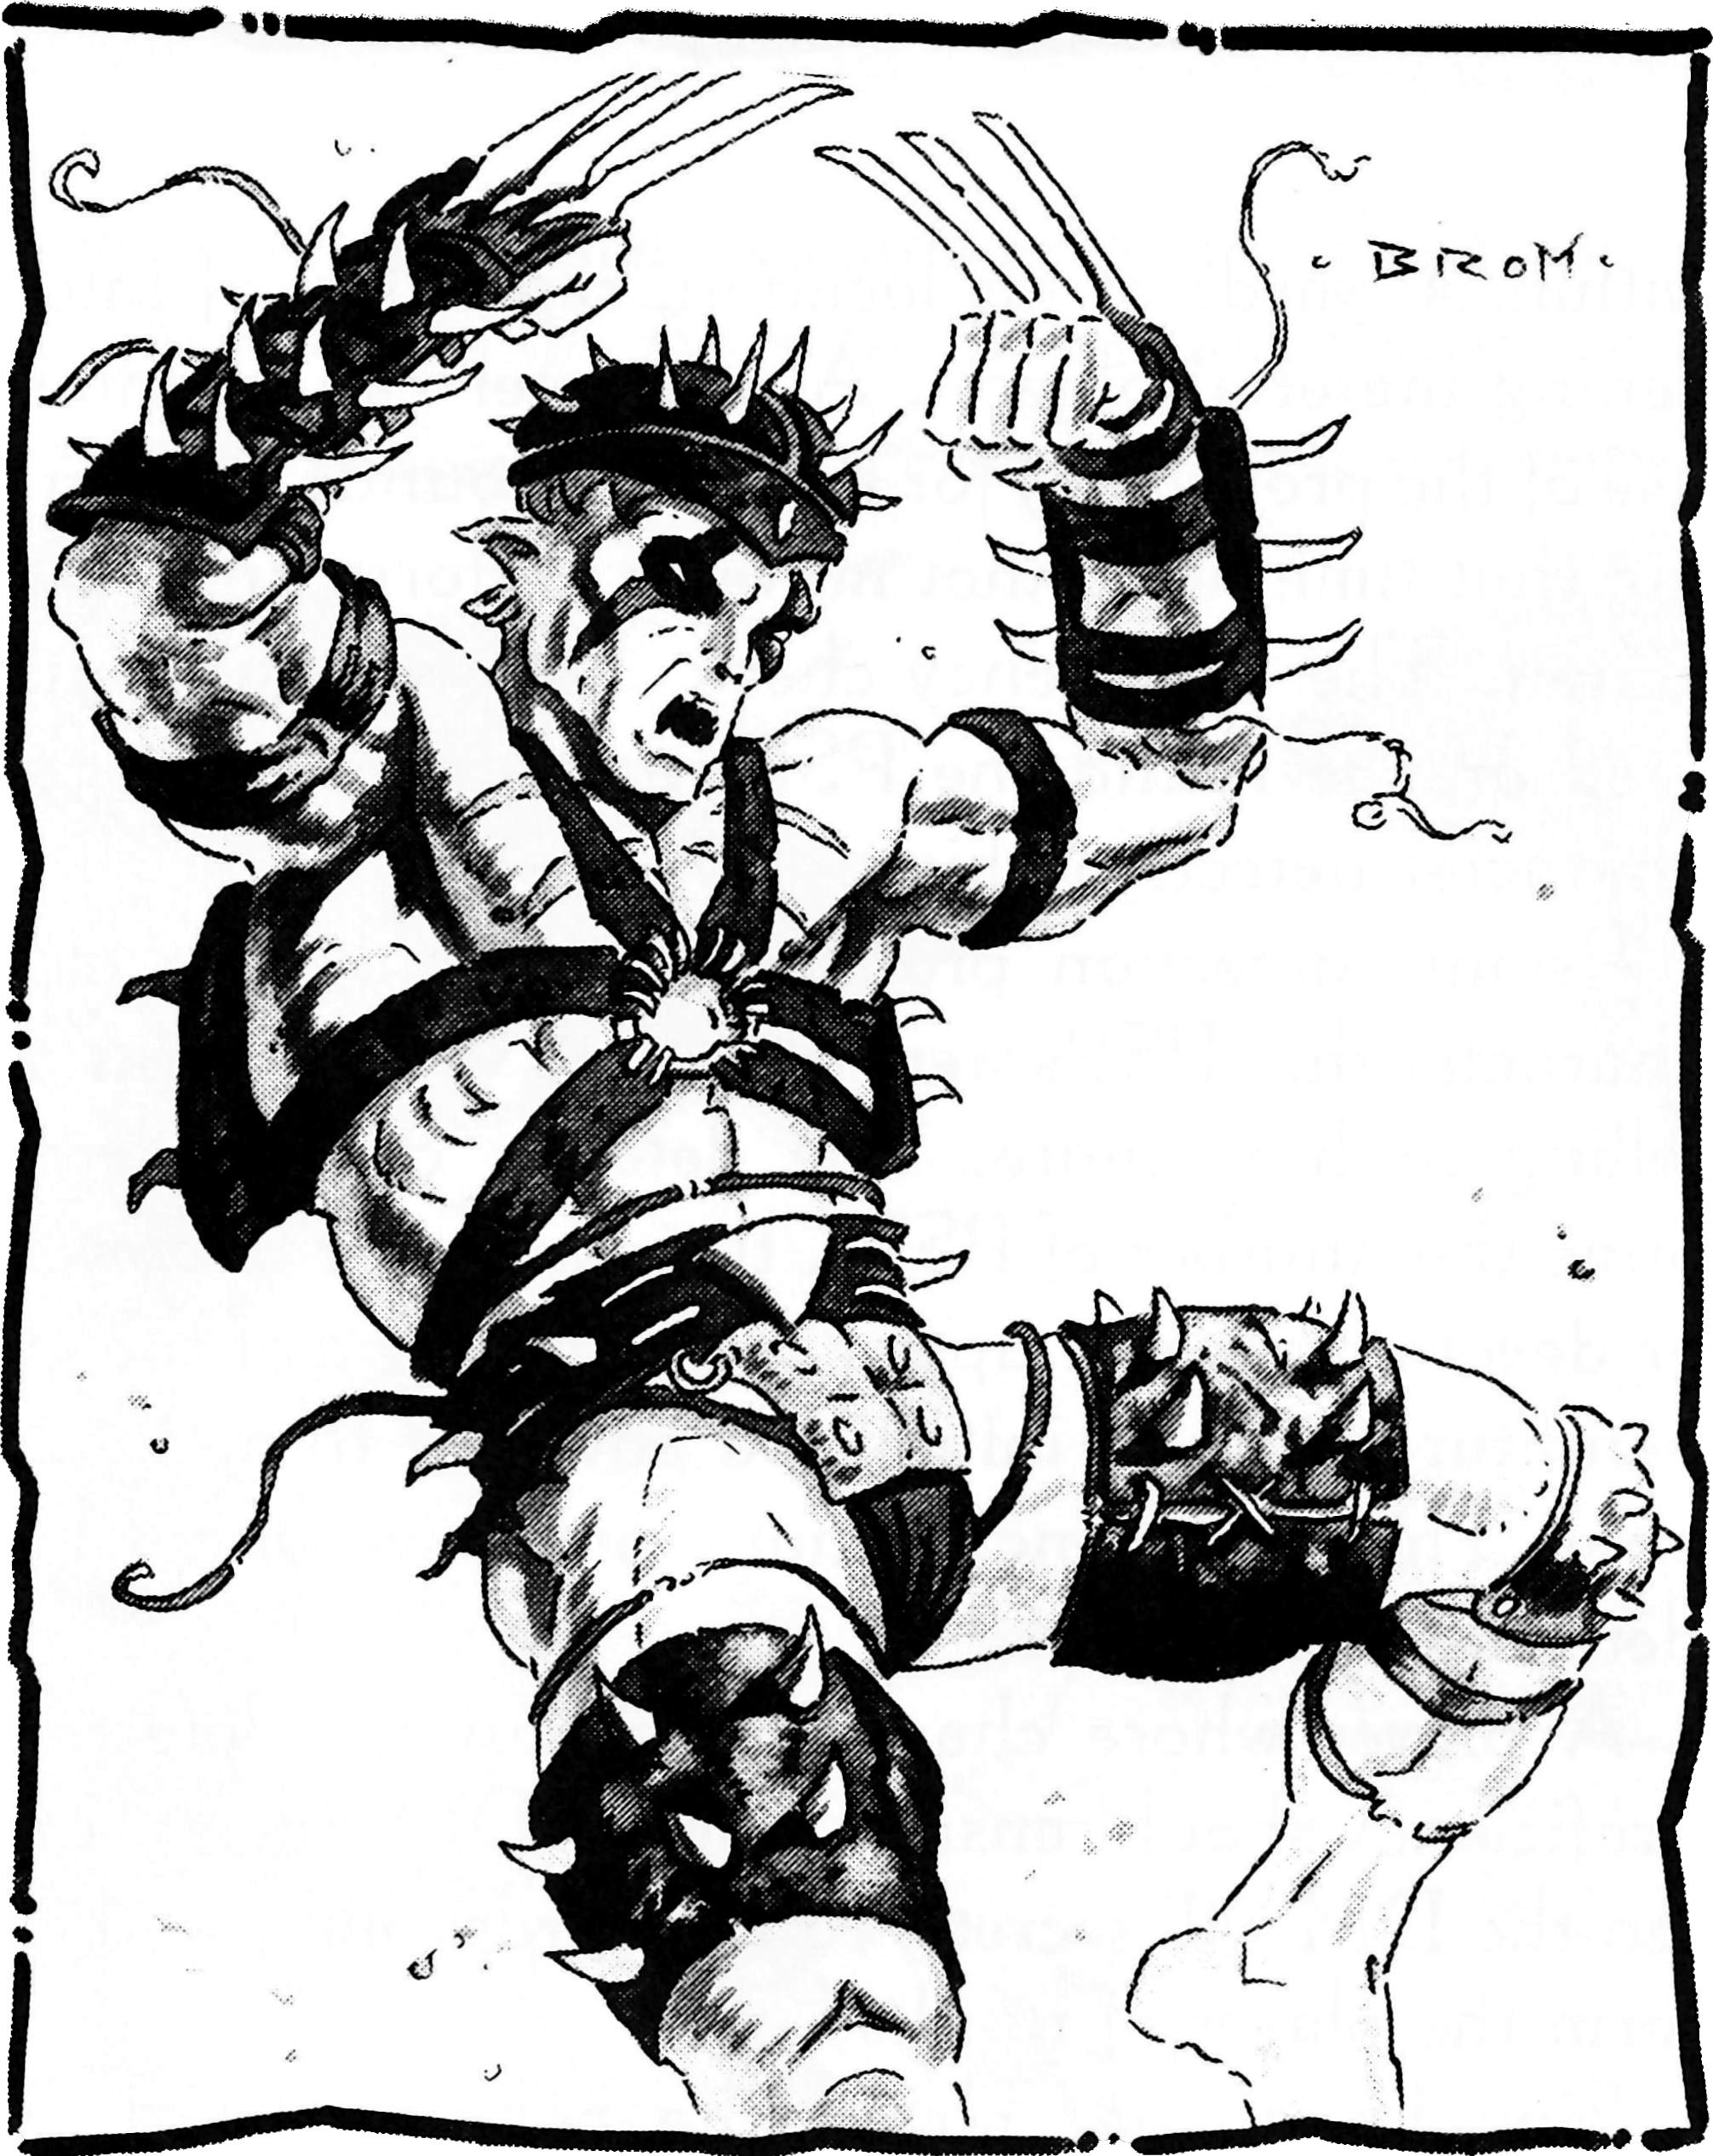
\includegraphics[width=\columnwidth]{images/barbarian-1.png}
\WOTC
\end{figure}

\subsection{Making a Barbarian}

The barbarian is a fearsome warrior, compensating for lack of training and discipline with bouts of powerful rage. While in this berserk fury, barbarians become stronger and tougher, better able to defeat their foes and withstand attacks. These rages leave barbarians winded; at first they only have the energy for a few such spectacular displays per day, but those few rages are usually sufficient.

\textbf{Races:} Humans are often barbarians, many having been raised in the wastes or escaped from slavery. Half-elves sometimes become barbarians, having been abandoned by their elven parents to the desert to survive on their own; if more of them survived they would be quite numerous. Dwarves are very rarely barbarians, but their mul half-children take to brutishness like a bird takes to flight, living by their wits and strengths in the wastes. Muls have a particular inclination this way of life, and very often ``go feral'' in the wilderness after escaping slavery in the city. Elves rarely take to the barbarian class; those that do are usually from raiding tribes such as the Silt Stalkers. Half-giants readily take the barbarian class. Despite their feral reputations, halflings rarely become barbarians; their small statures and weak strength adapts them better for the ranger class. Likewise, despite their wild nature, thri-kreen are rarely barbarians since their innate memories allow them to gain more specialized classes, such as ranger, without training. Pterrans of the Forest Ridge occasionally become barbarians, but like halflings they more often favor the ranger class.

\textbf{Alignment:} Barbarians are never lawful---their characteristic rage is anything but disciplined and controlled. Many barbarians in the cities are often rejects from the regular army, unable to bear regular discipline or training. Some may be honorable, but at heart they are wild. At best, chaotic barbarians are free and expressive. At worst, they are thoughtlessly destructive.

\subsection{Game Rule Information}
\textbf{Alignment:} Any nonlawful.

\textbf{Hit Die:} d12.

\subsubsection{Class Skills}
\skill{Autohypnosis} (Wis), \skill{Climb} (Str), \skill{Craft} (Int), \skill{Escape Artist} (Des), \skill{Handle Animal} (Cha), \skill{Intimidate} (Cha), \skill{Jump} (Str), \skill{Knowledge} (nature) (Int), \skill{Listen} (Wis), \skill{Profession} (Wis), \skill{Ride} (Dex), and \skill{Survival} (Wis).

\textbf{Skill Points per Level:} 4 + Int modifier ($\times4$ at 1st level).

\subsubsection{Class Features}

\textbf{Weapon and Armor Proficiency:} A barbarian is proficient with all simple and martial weapons, light armor, medium armor, and shields (except tower shields).

\textbf{Fast Movement (Ex):} A barbarian's land speed is faster than the norm for his race by +3 meters. This benefit applies only when he is wearing no armor, light armor, or medium armor and not carrying a heavy load. Apply this bonus before modifying the barbarian's speed because of any load carried or armor worn.

\textbf{Rage (Ex):} A barbarian can fly into a rage a certain number of times per day. In a rage, a barbarian temporarily gains a +4 bonus to Strength, a +4 bonus to Constitution, and a +2 morale bonus on Will saves, but he takes a $-2$ penalty to Armor Class. The increase in Constitution increases the barbarian's hit points by 2 points per level, but these hit points go away at the end of the rage when his Constitution  score drops back to normal. (These extra hit points are not lost first the way temporary hit points are.) While raging, a barbarian cannot use any Charisma-, Dexterity-, or Intelligence-based skills (except for \skill{Balance}, \skill{Escape Artist}, \skill{Intimidate}, and \skill{Ride}), the \skill{Concentration} skill, or any abilities that require patience or concentration, nor can he cast spells or activate magic items that require a command word, a spell trigger (such as a wand), or spell completion (such as a scroll) to function. He can use any feat he has except \feat{Combat Expertise}, item creation feats, and metamagic feats. A fit of rage lasts for a number of rounds equal to 3 + the character's (newly improved) Constitution modifier. A barbarian may prematurely end his rage. At the end of the rage, the barbarian loses the rage modifiers and restrictions and becomes fatigued ($-2$ penalty to Strength, $-2$ penalty to Dexterity, can't charge or run) for the duration of the current encounter (unless he is a 15th-level barbarian, at which point this limitation no longer applies).

A barbarian can fly into a rage only once per encounter. At 1st level he can use his rage ability once per day. At 4th level and every four levels thereafter, he can use it one additional time per day (to a maximum of six times per day at 20th level). Entering a rage takes no time itself, but a barbarian can do it only during his action, not in response to someone else's action. 

\textbf{Uncanny Dodge (Ex):} At 2nd level, a barbarian retains his Dexterity bonus to AC (if any) even if he is caught flat-footed or struck by an invisible attacker. However, he still loses his Dexterity bonus to AC if immobilized. If a barbarian already has uncanny dodge from a different class, he automatically gains improved uncanny dodge instead.

\textbf{Wasteland Trap Sense (Ex):} Starting at 3rd level, a barbarian gains a +1 bonus on Reflex saves made to avoid traps and natural hazards, and a +1 dodge bonus to AC against attacks made by traps and natural hazards. These bonuses rise by +1 every three barbarian levels thereafter (6th, 9th, 12th, 15th, and 18th level). Trap sense bonuses gained from multiple classes stack.

\textbf{Improved Uncanny Dodge (Ex):} At 5th level and higher, a barbarian can no longer be flanked. This defense denies a rogue the ability to sneak attack the barbarian by flanking him, unless the attacker has at least four more rogue levels than the target has barbarian levels. If a character already has uncanny dodge from a second class, the character automatically gains improved uncanny dodge instead, and the levels from the classes that grant uncanny dodge stack to determine the minimum level a rogue must be to flank the character.

\begin{figure}[t!]
\centering
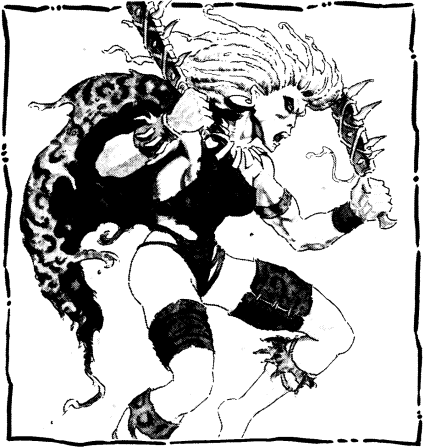
\includegraphics[width=\columnwidth]{images/halfling-1.png}
\WOTC
\end{figure}

\textbf{Damage Reduction (Ex):} At 7th level, a barbarian gains Damage Reduction. Subtract 1 from the damage the barbarian takes each time he is dealt damage from a weapon or a natural attack. At 10th level, and every three barbarian levels thereafter (13th, 16th, and 19th level), this damage reduction rises by 1 point. Damage reduction can reduce damage to 0 but not below 0.

\textbf{Bonus Feat:} At 8th level and every three levels thereafter (11th, 14th, 17th, and 20th level), a barbarian gains a bonus feat, which must be selected from the following list:
\feat{Awesome Blow},
\feat{Blind-Fight},
\feat{Cleave},
\feat{Closed Mind},
% \feat{Combat Reflexes},
Dash\textsuperscript{CW},
Destructive Rage\textsuperscript{CW},
\feat{Diehard},
\feat{Endurance},
Extend Rage\textsuperscript{CW},
Extra Rage\textsuperscript{CW},
% Faster Healing\textsuperscript{CW},
Fleet of Foot\textsuperscript{CW},
\feat{Great Cleave},
% \feat{Greater Critical},
Greater Resiliency\textsuperscript{CW},
\feat{Hard as Rock},
\feat{Hostile Mind},
\feat{Improved Bull Rush},
% \feat{Improved Critical},
% \feat{Improved Initiative},
\feat{Improved Sunder},
\feat{Innate Hunter},
Instantaneous Rage\textsuperscript{CW},
Intimidating Rage\textsuperscript{CW},
\feat{Mind Over Body},
\feat{Power Attack},
% \feat{Psionic Hole},
% \feat{Quick Draw},
\feat{Rapid Metabolism},
\feat{Reckless Offense},
\feat{Run},
Steadfast Determination\textsuperscript{PH2},
\feat{Toughness},
\feat{Track},
\feat{Wastelander}.
He must meet all the prerequisites for the feat.

\textbf{Greater Rage (Ex):} At 8th level, a barbarian's bonuses to Strength and Constitution during his rage each increase to +6, and his morale bonus on Will saves increases to +3. The penalty to AC remains at $-2$.

\textbf{Indomitable Will (Ex):} While in a rage, a barbarian of 13th level or higher gains a +4 bonus on Will saves to resist enchantment spells and telepathy powers. This bonus stacks with all other modifiers, including the morale bonus on Will saves he also receives during his rage.

\textbf{Tireless Rage (Ex):} At 15th level and higher, a barbarian no longer becomes fatigued at the end of his rage.

\textbf{Mighty Rage (Ex):} At 17th level, a barbarian's bonuses to Strength and Constitution during his rage each increase to +8, and his morale bonus on Will saves increases to +4. The penalty to AC remains at $-2$.

\subsubsection{Ex-Barbarians}
A barbarian who becomes lawful loses the ability to rage and cannot gain more levels as a barbarian. He retains all the other benefits of the class (damage reduction, fast movement, wasteland trap sense, and uncanny dodge).


\subsection{Playing a Barbarian}
All cower and stand in awe at the fury you can tap, enhancing your strength and toughness. But what do these people know of the burnt wastes of Athas, the hellish jungles of the Forest Ridge? The cruel vicissitudes of growing up in the wastes of Athas were nothing but normal to you. When your family was lost in a tembo attack, or when your entire village was either murdered or forced into slavery, how could you not know they might not had to die? These and many other brutal experiences marked you, and you now stand apart from those born into the ``comforts'' of the city-states.

\subsubsection{Religion}
Although most are profoundly superstitious, barbarians distrust the established elemental temples of the cities. Some worship the elements of fire or air or devote themselves to a famous figure. Most barbarians truly believe the sorcerer-kings to be gods, because of their undeniable power, and a few actually worship a sorcerer-king, usually the one that conquered their tribe. Such barbarians often escape menial slavery by joining an elite unit of barbarians in the service of an aggressive city-state such as Urik, Draj or Gulg.

\subsubsection{Other Classes}
Barbarians are most comfortable in the company of gladiators, and of clerics of Air and Fire. Enthusiastic lovers of music and dance, barbarians admire bardic talent, and some barbarians also express fascination with bardic poisons, antidotes and alchemical concoctions. With some justification, barbarians do not trust wizardry. Even though many barbarians manifest a wild talent, they tend to be wary of psions and Tarandan psionicists. Psychic warriors, on the other hand, are creatures after the barbarian's own heart, loving battle for its own sake. Barbarians have no special attitudes toward fighters or rogues. Barbarians admire gladiators and will ask about their tattoos and exploits, but will quickly grow bored if the gladiator does not respond boastfully.

\subsubsection{Combat}
You know that half the battle occurs before the fight even begins. You prefer to choose your battleground when you can, stalking your opponent into terrain that best suits your abilities. Once battle is joined, you become a wild frenzy of motion, striking quickly and powerfully until all your opponents are crushed. While you lack the training of the fighter, or the cunning of the gladiator, you more than compensate them through sheer power and resilience.

\subsubsection{Advancement}
Becoming a barbarian let you further tap into your feral nature, letting you become one with the savage beast in your hear, and through your training, you have learned what you must do to unlock it.

To fully utilize your barbarian abilities, you will want to focus on feats that take advantage of your superior strength and speed, such as Power Attack and Whirlwind Attack.


\subsection{Starting Packages}
\subsubsection{The Survivor}
Human Barbarian

\textbf{Ability Scores:} Str 15, Dex 13, Con 14, Int 10, Wis 12, Cha 8.

\textbf{Skills:} \skill{Climb}, \skill{Escape Artist}, \skill{Listen}, \skill{Survival}.

\textbf{Languages:} Common.

\textbf{Feat:} \feat{Great Fortitude}, \feat{Wastelander}.

\textbf{Weapons:} Carrikal (1d8/$\times$3)

Atlatl with 10 javelins (1d6/$\times$3, 12 m).

\textbf{Armor:} Scale mail (+4 AC).

\textbf{Gear:} Standard adventurer's kit, 13 cp.

\subsubsection{The Crusher}
Half-giant Barbarian

\textbf{Ability Scores:} Str 23, Dex 10, Con 18, Int 6, Wis 9, Cha 4.

\textbf{Skills:} \skill{Climb}, \skill{Intimidate}, \skill{Jump}.

\textbf{Languages:} Common.

\textbf{Feat:} \feat{Exotic Weapon Proficiency} (swatter).

\textbf{Weapons:} Swatter (3d8/$\times$4).

\textbf{Armor:} Leather (+2 AC).

\textbf{Gear:} Standard adventurer's kit, 0 cp.

\subsubsection{The Hunter}
Thri-kreen Barbarian

\textbf{Ability Scores:} Str 15, Dex 14, Con 12, Int 10, Wis 13, Cha 8.

\textbf{Skills:} \skill{Jump}, \skill{Knowledge} (nature), \skill{Search}, \skill{Survival}.

\textbf{Languages:} Kreen.

\textbf{Feat:} \feat{Track}.

\textbf{Weapons:} Four chatkchas (1d6, 6 m).

\textbf{Armor:} Heavy wooden shield (+2 AC).

\textbf{Gear:} Standard adventurer's kit, 13 cp.


\subsection{Barbarians on Athas}
\Quote{Don't make my friend angry. You won't like him when he's angry.}{Cabal, half-elven bard}

In a savage world like Athas, is only natural that some of its inhabitants have turned into barbarians. They are fierce combatants without the army training fighters receive or wild rangers without the hunting skills.

\subsubsection{Daily Life}
A barbarian is a passionate adventurer. As a survivalist, he often sees his involvement in a particular enterprise as a validation of his superior strength and resilience. In his mind, his presence alone is enough to ensure the success of a quest, adventure, or ruin raid. Even simple tasks are additional opportunities to prove his own worth by accomplishing the task with might and alacrity. Barbarians are typically hardheaded and unforgiving because of the rigors of his previous life.

\subsubsection{Notables}
It is rare for a barbarian to live long enough, or close enough to civilization, in order to become famous, but a few examples exist. Korno, a Raamite gladiator, became the leader of a group of slaves, and Korno's furious rage known from the arenas has only increased after losing everything in the Raam invasion by Dregoth. The leader of Pillage, Chilod, is a tarek know for his outbursts of rage and cruelty, being one of the most feared chiefs of the Bandit States.

\subsubsection{Organizations}
Because of their independent and sometimes downright chaotic natures, many barbarians refuse to join organizations of any kind, though they usually maintain relationships with trading houses and raiding tribes. There is no specific organization that binds barbarians together.

\subsubsection{NPC Reactions}
Many lay people cannot tell a barbarian from a ranger or a fighter until his rage overcomes him and he starts screaming and bashing. Most authority figures and templars do not appreciate barbarians since they are prone to losing control and cannot be truly trusted. Thus, they generally treat barbarians with a great deal of caution.

\subsubsection{Barbarian Lore}
Characters with ranks in \skill{Knowledge} (nature) can research barbarians to learn more about them. When a character makes a skill check, read or paraphrase the following, including the information from lower DCs.

\textbf{DC 10:} Barbarians are hot-blooded combatants who fight with great brutality and savagery.

\textbf{DC 15:} Barbarians become stronger and more resilient when they lose control.

\textbf{DC 20:} Barbarians can stand up to punishment that no other individual can endure, and their reflexes are as quick as a rogue's.
\Class{Bard}
{Some people think a club can solve any problem. Unless you're a half-giant, there are more sophisticated ways of settling a disagreement.}{Cabal, half-elven bard}

From the shadowy corners of Athas' most disreputable places hails the bard. Like their counterparts in other fantasy worlds, Athasian bards are the unquestioned masters of oral tradition and forgotten lore, but rather than sharing their lore with whoever will listen, Athasian bards guard their secrets as jealously as the sorcerer-kings harbor their water and iron. Athasian bards may sell information to the highest bidder; they peddle their services and the fruits of their knowledge, but trade secrets are what give bards an edge on the uninitiated. Bards would rather die than reveal these secrets.

Meeting a bard can be an uneasy encounter, since one never knows how the bard has chosen to devote his multiple talents. Some bards master the art of making poisons, and survive by selling these poisons and their antidotes for those who have coin to pay. Some bards master the art of entertainment, using their performances to amuse nobles and templars and gain wealth. Some become assassins, mixing their knowledge of poison and stealth to become hired hands. Bards' unique position in the Athasian society means they often overhear conversations between high-ranking templars or nobles, or they may have treated an injured person that prefers to remain anonymous. Respectable folk despise them; the powerful fear them; but in the Athasian cities, everyone eventually comes to need their services.

\WarriorTable[b{0.8cm} b{2.6cm} Z{1.4cm} Z{1.4cm} Z{1.4cm} X]{The Bard}{
1st  & +0         & +2  & +2  & +2  & Bardic music, bardic knowledge, smuggler, countersong, \emph{fascinate}, inspire courage +1\\
2nd  & +1         & +3  & +3  & +3  & Poison use, streetsmart                                  \\
3rd  & +2         & +3  & +3  & +3  & Inspire competence, \feat{Quick Draw}                    \\
4th  & +3         & +4  & +4  & +4  & Trade secret                                             \\
5th  & +3         & +4  & +4  & +4  & Mental resistance                                        \\
6th  & +4         & +5  & +5  & +5  & Improved poison use, \emph{suggestion}, quick thinking +2\\
7th  & +5         & +5  & +5  & +5  & Chance 1/day, inspire courage +2                         \\
8th  & +6/+1      & +6  & +6  & +6  & Trade secret                                             \\
9th  & +6/+1      & +6  & +6  & +6  & Inspire greatness, speed reactions                       \\
10th & +7/+2      & +7  & +7  & +7  & Special ability                                          \\
11th & +8/+3      & +7  & +7  & +7  & Quick thinking +4                                        \\
12th & +9/+4      & +8  & +8  & +8  & \emph{Song of freedom}, trade secret                     \\
13th & +9/+4      & +8  & +8  & +8  & Inspire courage +3                                       \\
14th & +10/+5     & +9  & +9  & +9  & Chance 2/day                                             \\
15th & +11/+6/+1  & +9  & +9  & +9  & Inspire heroics, special ability                         \\
16th & +12/+7/+2  & +10 & +10 & +10 & Quick thinking +6, trade secret                          \\
17th & +12/+7/+2  & +10 & +10 & +10 & Awareness                                                \\
18th & +13/+8/+3  & +11 & +11 & +11 & \emph{Mass suggestion}, \emph{mind blank}                \\
19th & +14/+9/+4  & +11 & +11 & +11 & Inspire courage +4                                       \\
20th & +15/+10/+5 & +12 & +12 & +12 & Special ability, trade secret                            \\
}

\Figure*{t}{images/bard-2.png}

\subsection{Making a Bard}
Bards receive numerous abilities they can use to survive. Many become masters of poisons, selling their illegal substances to anyone. Alone of the classes, bards hold the secrets of alchemy, creating fiery concoctions and mysterious mixes. Bards are master smugglers, selling spell components and other illegal items in the Bard's Quarters of the city-states. All bards, however, have some degree of entertainment skill. The songs of most bards can dazzle a crowd, or incite them to riot. Bards tend to learn to play a variety of instruments, or recite poetry or old legends by campfire. They can be acrobats, performing dazzling displays of physical prowess. They are often called upon as sources of information.

\textbf{Abilities:} Charisma is the most important ability for a bard, because many of their abilities and skills are affected by it. A high Dexterity improves the bard's defensive ability. Intelligence is also important because it bolster the numbers of skills he has access.

\textbf{Races:} All humanoid races of Athas can become bards. The social stigma in certain regions may be higher than others, however. For example, the loremasters of the halflings of the Jagged Cliffs are highly regarded because of the ancient secrets and histories they preserve. But in the city-states, where the Bard's Quarters are notorious, being a bard is not usually a good thing. Elven tribes often have a bard, who keeps the history of the tribe alive, its conquests and defeats. Humans are often bards, becoming performers of great talent, or assassins of deadly skill and precision. Half-elves, because of their lonely existence, often take to being bards. The prejudice they face at every stage in life can move some to become great poets or singers. Muls and half-giants make poor bards; their talents are usually better served elsewhere than the stage or the shadows of alleys. As well, thri-kreen are rarely seen as bards, relying instead upon their racial memory.

\textbf{Alignment:} Most bards are chaotic, and operate alone, brokering information, arranging deals, smuggling illegal wares such as poisons, drugs, spell components and other things. Neutral bards are the ones most likely to operate in fellowships with adventurers, or entertain in troupes with other bards. The rare lawful bards can easily secure positions as councilors or agents for templars, and noble and merchant houses. Good bards are often entertainers or lorekeepers, putting their talents to benevolent use, sometimes diagnosing poisonings and selling the proper antidotes. Evil bards are often masters of poisons and alchemy, selling their wares to anyone with the ceramic to pay.

\subsection{Game Rule Information}

\textbf{Hit Die:} d6.

\subsubsection{Class Skills}
\skill{Appraise} (Int), \skill{Balance} (Dex), \skill{Bluff} (Cha), \skill{Climb} (Str), \skill{Craft} (Int), \skill{Decipher Script} (Int), \skill{Diplomacy} (Cha), \skill{Disguise} (Cha), \skill{Escape Artist} (Dex), \skill{Forgery} (Int), \skill{Gather Information} (Cha), \skill{Heal} (Wis), \skill{Hide} (Dex), \skill{Intimidate} (Cha), \skill{Jump} (Str), \skill{Knowledge} (all skills individually) (Int), \skill{Listen} (Wis), \skill{Move Silently} (Dex), \skill{Perform} (Cha), \skill{Profession} (Wis), \skill{Ride} (Dex), \skill{Search} (Int), \skill{Sense Motive} (Wis), \skill{Sleight of Hand} (Dex), \skill{Speak Language} (N/A), \skill{Tumble} (Dex), \skill{Use Magic Device} (Cha), \skill{Use Psionic Device} (Cha), and \skill{Use Rope} (Dex).

\textbf{Skill Points per Level:} 6 + Int modifier ($\times4$ at 1st level).

\subsubsection{Class Features}

\textbf{Weapon and Armor Proficiency:} You are proficient in all simple weapons, plus the bard's friend, all crossbows, garrote, greater blowgun, whip and widow's knife. You are proficient in light armor, but not shields.

\textbf{Bardic Knowledge:} A bard may make a special bardic knowledge check with a bonus equal to his bard level + his Intelligence modifier to see whether he knows some relevant information about local notable people, legendary items, or noteworthy places. (If the bard has 5 or more ranks in \skill{Knowledge} (history), he gains a +2 bonus on this check.)

A successful bardic knowledge check will not reveal the powers of a magic item but may give a hint as to its general function. A bard may not take 10 or take 20 on this check; this sort of knowledge is essentially random.

\Table{}{p{0.6cm} X}{
\tableheader DC & \tableheader Type of Knowledge\\
10 & Common, known by at least a substantial minority of the local population.\\
20 & Uncommon but available, known by only a few people legends.\\
25 & Obscure, known by few, hard to come by.\\
30 & Extremely obscure, known by very few, possibly forgotten by most who once knew it, possibly known only by those who don't understand the significance of the knowledge.}

\textbf{Bardic Music:} Once per day per bard level, a bard can use his song or poetics to produce magical effects on those around him (usually including himself, if desired). While these abilities fall under the category of bardic music and the descriptions discuss singing or playing instruments, they can all be activated by reciting poetry, chanting, singing lyrical songs, singing melodies, whistling, playing an instrument, or playing an instrument in combination with some spoken performance. Each ability requires both a minimum bard level and a minimum number of ranks in the \skill{Perform} skill to qualify; if a bard does not have the required number of ranks in at least one \skill{Perform} skill, he does not gain the bardic music ability until he acquires the needed ranks. A bard cannot use \skill{Perform} (arena fighting) to use his bardic music abilities.

Starting a bardic music effect is a standard action. Some bardic music abilities require concentration, which means the bard must take a standard action each round to maintain the ability. Even while using bardic music that doesn't require concentration, a bard cannot cast spells, activate magic items by spell completion (such as scrolls), spell trigger (such as wands), or command word. Just as for casting a spell with a verbal component, a deaf bard has a 20\% chance to fail when attempting to use bardic music. If he fails, the attempt still counts against his daily limit.

\textit{Countersong (Su):} A bard with 3 or more ranks in a \skill{Perform} skill can use his music or poetics to counter magical effects that depend on sound (but not spells that simply have verbal components). Each round of the countersong, he makes a \skill{Perform} check. Any creature within 9 meters of the bard (including the bard himself) that is affected by a sonic or language-dependent magical attack may use the bard's \skill{Perform} check result in place of its saving throw if, after the saving throw is rolled, the \skill{Perform} check result proves to be higher. If a creature within range of the countersong is already under the effect of a noninstantaneous sonic or language-dependent magical attack, it gains another saving throw against the effect each round it hears the countersong, but it must use the bard's \skill{Perform} check result for the save. Countersong has no effect against effects that don't allow saves. The bard may keep up the countersong for 10 rounds.

\textit{Fascinate (Sp):} A bard with 3 or more ranks in a \skill{Perform} skill can use his music or poetics to cause one or more creatures to become fascinated with him. Each creature to be fascinated must be within 27 meters, able to see and hear the bard, and able to pay attention to him. The bard must also be able to see the creature. The distraction of a nearby combat or other dangers prevents the ability from working. For every three levels a bard attains beyond 1st, he can target one additional creature with a single use of this ability.

To use the ability, a bard makes a \skill{Perform} check. His check result is the DC for each affected creature's Will save against the effect. If a creature's saving throw succeeds, the bard cannot attempt to fascinate that creature again for 24 hours. If its saving throw fails, the creature sits quietly and listens to the song, taking no other actions, for as long as the bard continues to play and concentrate (up to a maximum of 1 round per bard level). While fascinated, a target takes a $-4$ penalty on skill checks made as reactions, such as \skill{Listen} and \skill{Spot} checks. Any potential threat requires the bard to make another \skill{Perform} check and allows the creature a new saving throw against a DC equal to the new \skill{Perform} check result.

Any obvious threat, such as someone drawing a weapon, casting a spell, or aiming a ranged weapon at the target, automatically breaks the effect. Fascinate is an enchantment (compulsion), mind-affecting ability.

\textit{Inspire Courage (Su):} A bard with 3 or more ranks in a \skill{Perform} skill can use song or poetics to inspire courage in his allies (including himself), bolstering them against fear and improving their combat abilities. To be affected, an ally must be able to hear the bard sing. The effect lasts for as long as the ally hears the bard sing and for 5 rounds thereafter. An affected ally receives a +1 morale bonus on saving throws against charm and fear effects and a +1 morale bonus on attack and weapon damage rolls. At 7th level, and every six bard levels thereafter, this bonus increases by 1 (+2 at 7th, +3 at 13th, and +4 at 19th). Inspire courage is a mind-affecting ability.

\textit{Inspire Competence (Su):} A bard of 3rd level or higher with 6 or more ranks in a \skill{Perform} skill can use his music or poetics to help an ally succeed at a task. The ally must be within 9 meters and able to see and hear the bard. The bard must also be able to see the ally.

The ally gets a +2 competence bonus on skill checks with a particular skill as long as he or she continues to hear the bard's music. Certain uses of this ability are infeasible. The effect lasts as long as the bard concentrates, up to a maximum of 2 minutes. A bard can't inspire competence in himself. Inspire competence is a mind-affecting ability.

\textit{Suggestion (Sp):} A bard of 6th level or higher with 9 or more ranks in a \skill{Perform} skill can make a \spell{suggestion} (as the spell) to a creature that he has already fascinated. Using this ability does not break the bard's concentration on the fascinate effect, nor does it allow a second saving throw against the fascinate effect.

Making a \emph{suggestion} doesn't count against a bard's daily limit on bardic music \skill{perform}ances. A Will saving throw (DC 10 + \onehalf bard's level + bard's Cha modifier) negates the effect. This ability affects only a single creature (but see \emph{mass suggestion}, below). \emph{Suggestion} is an enchantment (compulsion), mind-affecting, language dependent ability.

\textit{Inspire Greatness (Su):} A bard of 9th level or higher with 12 or more ranks in a \skill{Perform} skill can use music or poetics to inspire greatness in himself or a single willing ally within 9 meters, granting him or her extra fighting capability. For every three levels a bard attains beyond 9th, he can target one additional ally with a single use of this ability (two at 12th level, three at 15th, four at 18th). To inspire greatness, a bard must sing and an ally must hear him sing. The effect lasts for as long as the ally hears the bard sing and for 5 rounds thereafter. A creature inspired with greatness gains 2 bonus Hit Dice (d10s), the commensurate number of temporary hit points (apply the target's Constitution modifier, if any, to these bonus Hit Dice), a +2 competence bonus on attack rolls, and a +1 competence bonus on Fortitude saves. The bonus Hit Dice count as regular Hit Dice for determining the effect of spells that are Hit Dice dependent. Inspire greatness is a mind-affecting ability.

\textit{Song of Freedom (Sp):} A bard of 12th level or higher with 15 or more ranks in a \skill{Perform} skill can use music or poetics to create an effect equivalent to the \spell{break enchantment} spell (caster level equals the character's bard level). Using this ability requires 1 minute of uninterrupted concentration and music, and it functions on a single target within 9 meters. A bard can't use song of freedom on himself.

\Figure{t}{images/bard-1.png}

\textit{Inspire Heroics (Su):} A bard of 15th level or higher with 18 or more ranks in a \skill{Perform} skill can use music or poetics to inspire tremendous heroism in himself or a single willing ally within 9 meters. For every three bard levels the character attains beyond 15th, he can inspire heroics in one additional creature. To inspire heroics, a bard must sing and an ally must hear the bard sing for a full round. A creature so inspired gains a +4 morale bonus on saving throws and a +4 dodge bonus to AC. The effect lasts for as long as the ally hears the bard sing and for up to 5 rounds thereafter. Inspire heroics is a mind-affecting ability.

\textit{Mass Suggestion (Sp):} This ability functions like \emph{suggestion}, above, except that a bard of 18th level or higher with 21 or more ranks in a \skill{Perform} skill can make the suggestion simultaneously to any number of creatures that he has already fascinated. \emph{Mass suggestion} is an enchantment (compulsion), mind-affecting, language-dependent ability.

\textbf{Smuggler (Ex):} A bard receives a +1 insight bonus to \skill{Bluff} and \skill{Sleight of Hand} checks for every two bard levels.

\textbf{Poison Use:} Bards are trained in the use of poisons, and as of 2nd level, never risk accidentally poisoning themselves when applying poison to a blade.

\textbf{Streetsmart (Ex):} When a bard reaches 2nd level, he gets a +2 competence bonus to \skill{Gather Information} and \skill{Intimidate} checks.

\textbf{Quick Draw:} Bards learn to strike quickly and without warning. At 3rd level, a bard gains \feat{Quick Draw} as a bonus feat.

\textbf{Trade Secrets:} At 4th level and every four levels thereafter (8th, 12th, 16th, and 20th level), a bard learns a trade secret chosen from the list below.

\textit{Alchemy Dealer (Ex):} A bard with this trade secret pays \onehalf of the market price for raw materials needed to craft alchemical items.

\textit{Coolheaded:} A bard with this trade secret may take 10 on \skill{Bluff} and \skill{Diplomacy} checks. A bard must be at least 12th level to select this trade secret.

\textit{Improvised Materials (Ex):} A bard with this trade secret can craft poisons from raw materials at hand instead of relying on specific ingredients. Doing so increases the \skill{Craft} (poisonmaking) check DC by 5 but otherwise has no effect on the poison's potency.

\textit{Poison Dealer (Ex):} A bard with this trade secret pays \onehalf of the market price for raw materials needed to craft poisons.

\textit{Poisonbane (Ex):} A bard with this trade secret receives a +4 insight bonus to \skill{Craft} (alchemy) checks when creating antitoxin and poison antidotes.

\textit{Poison Resistance (Ex):} A bard with this trade secret receives a +4 bonus to saving throws against poisons.

\textit{Scorpion's Touch:} A bard with this trade secret adds +1 to the save DC of all poisons applied by him. This trade secret may be chosen more than once, and its effects stack.

\textit{Skilled:} A bard with this trade secret adds \onequarter your bard level as a competence bonus to one of the following skills: \skill{Appraise}, \skill{Bluff}, \skill{Craft}, \skill{Diplomacy}, \skill{Heal}, \skill{Perform}, \skill{Profession}, \skill{Sense Motive} or \skill{Sleight of Hand}. This trade secret may be chosen more than once, each time it applies to a different skill.

\textit{Smokestick Application (Ex):} A bard with this trade secret can combine inhaled poisons with smokesticks. All creatures within the area the smokestick covers (3-m cube) are affected by the poison you applied to the smokestick.

\textit{Versatile:} A bard with this trade secret selects any two non-class skills to be considered class skills.


\textbf{Mental Resistance (Ex):} Bards carry many dark secrets they would prefer remain secret. This, combined with a large amount of knowledge based on half-truths and false rumors makes your mind unreliable to those who would seek to mentally affect it. A 5th level bard receives a +2 morale bonus to saves made against telepathic powers and enchantment (charm) spells.

\textbf{Improved Poison Use (Ex):} At 6th level, a bard can apply poison to a weapon as a free action without provoking attacks of opportunity.

\textbf{Quick Thinking (Ex):} Bards often find themselves in a tight spot where they have to act quickly, whether it is to escape a templar patrol or strike first when in confrontation with a foe. At 6th level, a bard gets a +2 bonus on initiative checks. This bonus increases by 2 at every five levels thereafter (+4 at 11th, and +6 at 16th level).

\textbf{Chance (Ex):} Bards live on the edge in many ways. At 7th level, a bard may reroll one single d20 roll once per day, but have to keep the latter result---for better or for worse. At 14th level, a bard may use this ability two times per day.

\textbf{Speed Reactions (Ex):} Beginning at 9th level, when a bard uses the attack action or full attack action in melee, he may subtract a number from all melee attack rolls and add the same number to his initiative. This number may not exceed his base attack bonus. He may not make ranged attacks this round. The initiative increase takes effect on the next round. The new initiative is his initiative for the remainder of the combat, unless you were to use speed reactions again, which would increase your initiative further.

\textbf{Special Ability:} On attaining 10th level, and at every five levels thereafter (15th, and 20th), a bard gains a special ability of his choice from among the following options.

\textit{Defensive Roll (Ex):} A bard learns how to avoid a potentially lethal blow to take less damage from it than he otherwise would. Once per day, when he would be reduced to 0 or fewer hit points by damage in combat (from a weapon or other blow, not a spell or special ability), the bard can attempt to roll with the damage. To use this ability, the bard must attempt a Reflex saving throw (DC = damage dealt). If the save succeeds, he takes only half damage from the blow; if it fails, he takes full damage. He must be aware of the attack and able to react to it in order to execute his defensive roll---if he is denied his Dexterity bonus to AC, he can't use this ability. Since this effect would not normally allow a character to make a Reflex save for half damage, the rogue's evasion ability does not apply to the defensive roll.

\textit{Infiltrator (Ex):} When trying to mimic another person's speech, writing, and behavior, the bard roll the checks for \skill{Bluff}, \skill{Disguise} and \skill{Forgery} with advantage. This ability only works for the first time he tries to impersonate.

\textit{Silver Tongue (Ex):} His constant dealing with others gives him a keen sense of how to make them believe his lies. A bard may attempt a retry of one of the following skills, but with disadvantage: \skill{Bluff}, \skill{Diplomacy}, \skill{Disguise}, or \skill{Intimidate}. A bard may gain this special ability multiple times, selecting an additional skill for it to apply to each time.

\textit{Slippery Mind (Ex):} If a bard with slippery mind is affected by an enchantment spell or effect or a telepathy power or effect and fails his saving throw, he can attempt it again 1 round later at the same DC. He gets only this one extra chance to succeed on his saving throw.

\textbf{Awareness (Ex):} At 17th level, you are never caught flat-footed and always act in the surprise round.

\textit{Mind Blank (Sp):} At 18th level your mind becomes completely sealed against involuntary intrusion as per the \spell{mind blank} spell. This spell-like ability is always considered active.


\subsection{Playing a Bard}
You are a master of oral tradition and lore, and a true artist, but you share your talents only with those who can afford to pay you.

You are an artist. You are the center of attention (whenever you want to), the person everyone wants to talk to, the ``face'' of the party. Even if you aren't the most attractive or charismatic member of your group, your unequaled skill at performance arts creates an irresistible appeal born of justified confidence. You are more than just light entertainment, though. Your target rarely survives the encounter if you don't want him to.

You might adventure because you desire entertainment. Someone with your smarts gets bored easily. Alternatively, you may have been blacklisted on your current location because of a ``business transaction'' gone wrong. You have to keep moving, and adventuring offers you a regular change of scenery. In any case, a life of adventure allows you to see new things, meet interesting people, and get some silvers in the process.

\subsubsection{Religion}
No central bardic organization exists, and more often than not bards have no particular penchant for religion. Some may worship the elements, fearing the power of the elemental forces, and most bards tend to relate to the Air ever-changing nature, but bards that worship sorcerer-kings are rare. A lifestyle of breaking the rules of the city-states does not lend one to worship the lawgivers.

\subsubsection{Other Classes}
Bards face life as it comes, and usually hold no special grudge or awe for any one class. They usually approach other's profession on the basis of how it can help them at the moment. Clerics and druids are respected for their devotion to a divine force, but usually not held in awe. Fighters, gladiators and rangers can be useful as sword-arms but are otherwise useless to the bard. Bards do not view wizards with the same aversion as others might view them, since bards sell them their components.

\subsubsection{Combat}
A bard rarely seeks to initiate combat---instead he skulks about, looking for an opportunity to strike swiftly, using his poisons to their greatest advantage. Your work best with teammates, maneuvering to get flanks and help bring down opponents with your various poisons. Use your bardic music to bolster your allies and distract your opponents while the real heavy hitters in your group mop them up.

\subsubsection{Advancement}
You have a flexibility in building your talents unrivaled by any other class. You can either emphasize on ability or nurse a broad range of abilities. In most cases, feats that consistently improve your talents are more useful than feats that function in only certain situations.

% Many feats in the Athasian Emporium supplement make the most of your poison abilities. 
As you advance in the class, continue to max out your ranks in \skill{Bluff} and \skill{Perform}, and invest skill points in \skill{Gather Information} and \skill{Sleight of Hand}. \feat{Improved Feint} is an excellent choice with your expertise in \skill{Bluff}, and \feat{Greasing the Wheels} if perfect for getting around templar inspections. If you play up the assassin aspect of this class, consider magic (or psionic) items that help you cloak your true intentions, such as an amulet of proof against detection and location or a veil of lies.

When multiclassing or taking a level in a prestige class, find combinations that further broaden your abilities or that increase your flexibility. The prestige classes \class{Poisonmaster}, \class{Dune Trader}, and \class{Assassin} deserve special mention. They are a great combination with the bard class.


\subsection{Starting Packages}
\subsubsection{The Assassin}
Elf Bard

\textbf{Ability Scores:} Str 13, Dex 17, Con 10, Int 10, Wis 14, Cha 8.

\textbf{Skills:} \skill{Climb}, \skill{Disguise}, \skill{Hide}, \skill{Move Silently}, \skill{Open Lock}, \skill{Spot}.

\textbf{Languages:} Elven, Common.

\textbf{Feat:} \feat{Stealthy}.

\textbf{Weapons:} Bard's friend (1d4/18-20)

Shortbow with 20 arrows (1d6/$\times$3, 18 m).

\textbf{Armor:} Studded leather (+3 AC).

\textbf{Gear:} Standard adventurer's kit, thieves' tools, musical instrument, 9 cp.

\subsubsection{The Information Smuggler}
Human Bard

\textbf{Ability Scores:} Str 8, Dex, 12, Con 10, Int 15, Wis 14, Cha 13.

\textbf{Skills:} \skill{Bluff}, \skill{Decipher Script}, \skill{Diplomacy}, \skill{Gather Information}, \skill{Knowledge} (local), \skill{Listen}, \skill{Sense Motive}.

\textbf{Languages:} City language, Common, Elven.

\textbf{Feat:} \feat{Investigator}, \feat{Negotiator}.

\textbf{Weapons:} Widow's knife (1d4/$\times$3)

Light crossbow with 20 bolts (1d8/19-20, 24 m).

\textbf{Armor:} Leather armor (+2 AC).

\textbf{Gear:} Standard adventurer's kit, 4 cp.

\subsubsection{The Poisoner}
Half-elf Bard

\textbf{Ability Scores:} Str 8, Dex 15, Con 10, Int 15, Wis 14, Cha 6.

\textbf{Skills:} \skill{Appraise}, \skill{Craft} (alchemy), \skill{Craft} (poisonmaking), \skill{Knowledge} (local), \skill{Sleight of Hand}.

\textbf{Languages:} City language, Common, Elven.

\textbf{Feat:} \feat{Skill Focus} (Craft [poisonmaking]).

\textbf{Weapons:} Bard's friend (1d4/18-20)

Blowgun with 20 needles (1, 3 m).

\textbf{Armor:} Shell armor (+4 AC).

\textbf{Gear:} Standard adventurer's kit, smokestick, 4 cp.


\subsection{Bards on Athas}
\Quote{She was a rare beauty: charming, graceful, talented. It's too bad she killed my boss.}{Talos, mul bodyguard}

Athasian bards use songs and tales as their tools of trade. A bard is a person of wit and camaraderie. Despite having few other talents to offer, the bard is a welcome source of entertainment and information across Athas. However, bards are noted to be extremely untrustworthy and even ruthless---they often sell their skills as assassins and poison alchemists to the highest bidder.

In the cities, bards often become tools of the nobility. They're commonly hired by one noble house and sent to another as a gift. The bards are sent not only to entertain, but usually to perform some other subtle task as well (such as robbery, espionage, or even assassination).

Nobles consider it rude to turn down the gift of a bard or bard company. However, when presented with a troop of bards from one's worst enemy, it's sometimes better to be rude and turn them away, for the consequences of their visit could be downright deadly. To get around this, the noble who hired them sometimes disguises their approach by having another noble send them. A very complicated collage of intrigue and deceit is often woven wherever bards are involved.

\subsubsection{Daily Life}
The way a bard behaves depends on his individual sense of morality. Some think nothing of adopting false identities, smuggling forbidden goods, or even coldblooded assassination. Other bards find themselves driven to use their skills to entertain and help people.

Bards can become great leaders. With their quick wits and great charisma, bards would be natural leaders were it not for their inconstancy. If a bard manages to earn the trust of companions, they value his leadership. Lacking that trust, a bard rarely leads for long.

\subsubsection{Notables}
Bards often gain notoriety for their deeds, although most prefer to remain behind false identities. The human bard only known as Wheelock has become a legend when it comes to creating poisons. Fyrian Wynder is a Tyrian half-elven bard notorious for his combination of bardic abilities and the Way, since his acting skills enable him to adopt several identities, while his psionic abilities provide a means of gaining access to secured areas and going unnoticed once he gets there.

\subsubsection{Organizations}
Bards don't organize together, but they often linger around the same places, which end up getting known as the Bard's Quarter in most city-states. A bard joining an organization probably has a specific goal (or target) in mind and rakes a position that best allows him to attain it. A long-term commitment to such a group rarely appeals to a bard.

\subsubsection{NPC Reactions}
Common folk ten to have a hard time differentiating bards from rogues. Bards further confuse the issue by regularly adopting false identities and hiding their varied abilities. Thus, the reaction a bard gets from those he meets depends on what he is pretending to be at a time. Individuals who know about the bard class and the reputation that comes with it have an initial attitude one step more hostile than normal. Templars in particular look poorly upon bards, since they know of the various illegal activities they usually perform.

\subsubsection{Bard Lore}
Characters with ranks in \skill{Knowledge} (local) can research bards to learn more about them. When a character makes a skill check, read or paraphrase the following, including the information from lower DCs.

\textbf{DC 15:} Bards are jacks of all trades, masters of performance and deception, and information smugglers.

\textbf{DC 20:} Bards are masters of poisons and lore, and they have many of the skills of rogues.
\Class{Cleric}
{Without destruction, there is nothing to build.}{Credo of the fire cleric}

In a world without gods, spiritualism on Athas has unlocked the secrets of the raw forces of which the very planet is comprised: earth, air, fire, and water. However, other forces exist which seek to supplant them and rise to ascendancy in their place. These forces have taken up battle against the elements of creation on the element's own ground in the form of entropic perversions of the elements themselves: magma, rain, silt and sun.

\SpellcasterTable{The Cleric}{.5cm}{
1 & +0 & +2 & +0 & +2 & Pact, turn or rebuke undead & 3 & 1+1 &  &  &  &  &  &  &  &  \\
2 & +1 & +3 & +0 & +3 &  & 4 & 2+1 &  &  &  &  &  &  &  &  \\
3 & +2 & +3 & +1 & +3 &  & 4 & 2+1 & 1+1 &  &  &  &  &  &  &  \\
4 & +3 & +4 & +1 & +4 &  & 5 & 3+1 & 2+1 &  &  &  &  &  &  &  \\
5 & +3 & +4 & +1 & +4 &  & 5 & 3+1 & 2+1 & 1+1 &  &  &  &  &  &  \\
6 & +4 & +5 & +2 & +5 &  & 5 & 3+1 & 3+1 & 2+1 &  &  &  &  &  &  \\
7 & +5 & +5 & +2 & +5 &  & 6 & 4+1 & 3+1 & 2+1 & 1+1 &  &  &  &  &  \\
8 & +6/+1 & +6 & +2 & +6 &  & 6 & 4+1 & 3+1 & 3+1 & 2+1 &  &  &  &  &  \\
9 & +6/+1 & +6 & +3 & +6 &  & 6 & 4+1 & 4+1 & 3+1 & 2+1 & 1+1 &  &  &  &  \\
10 & +7/+2 & +7 & +3 & +7 &  & 6 & 4+1 & 4+1 & 3+1 & 3+1 & 2+1 &  &  &  &  \\
11 & +8/+3 & +7 & +3 & +7 &  & 6 & 5+1 & 4+1 & 4+1 & 3+1 & 2+1 & 1+1 &  &  &  \\
12 & +9/+4 & +8 & +4 & +8 &  & 6 & 5+1 & 4+1 & 4+1 & 3+1 & 3+1 & 2+1 &  &  &  \\
13 & +9/+4 & +8 & +4 & +8 &  & 6 & 5+1 & 5+1 & 4+1 & 4+1 & 3+1 & 2+1 & 1+1 &  &  \\
14 & +10/+5 & +9 & +4 & +9 &  & 6 & 5+1 & 5+1 & 4+1 & 4+1 & 3+1 & 3+1 & 2+1 &  &  \\
15 & +11/+6/+1 & +9 & +5 & +9 &  & 6 & 5+1 & 5+1 & 5+1 & 4+1 & 4+1 & 3+1 & 2+1 & 1+1 &  \\
16 & +12/+7/+2 & +10 & +5 & +10 &  & 6 & 5+1 & 5+1 & 5+1 & 4+1 & 4+1 & 3+1 & 3+1 & 2+1 &  \\
17 & +12/+7/+2 & +10 & +5 & +10 &  & 6 & 5+1 & 5+1 & 5+1 & 5+1 & 4+1 & 4+1 & 3+1 & 2+1 & 1+1 \\
18 & +13/+8/+3 & +11 & +6 & +11 &  & 6 & 5+1 & 5+1 & 5+1 & 5+1 & 4+1 & 4+1 & 3+1 & 3+1 & 2+1 \\
19 & +14/+9/+4 & +11 & +6 & +11 &  & 6 & 5+1 & 5+1 & 5+1 & 5+1 & 5+1 & 4+1 & 4+1 & 3+1 & 2+1 \\
20 & +15/+10/+5 & +12 & +6 & +12 &  & 6 & 5+1 & 5+1 & 5+1 & 5+1 & 5+1 & 4+1 & 4+1 & 3+1 & 3+1}


\subsection{Making a Cleric}
Clerics are the masters of elemental forces; they possess unique supernatural abilities to direct and harness elemental energy, and cast elemental spells. All things are comprised of the four elements in some degree, thus clerics can use their elemental powers to heal or harm others. Due to their affinities with the elements, clerics possess a number of supernatural elemental abilities. Though dimly understood, there exists a connection between elemental forces and the nature of undeath. Clerics can turn away, control, or even destroy undead creatures. Athas is a dangerous world; this practicality dictates that clerics must be able to defend themselves capably. Clerics are trained to use simple weapons and, in some cases, martial weapons; they are also taught to wear and use armor, since wearing armor does not interfere with elemental spells as it does arcane spells.

\textbf{Races:} All races include clerics in their societies, though each race possesses different perspectives regarding what a cleric's role involves. As masters of myth and the elemental mysteries, most clerics hold a place of reverence within their respective societies. However, more than a few races have varying affinities for one element over another. Dwarves almost always become earth clerics, a connection they've shared since before they were driven from their halls under the mountains. Dwarven determination and obsessive dedication matches perfectly with the enduring earth. Elves most often revere water, fire, or the winds; as nomads, they seldom feel a deep-seated affinity for the land. Thri-kreen are known to ally with all elements to the exclusion of fire. This seems to stem from a mistrust of flame, which is common in many kreen.

\textbf{Alignment:} Attaining the abilities of a true servant of the elements requires a deep understanding of the chosen kind of element of paraelement. An aspiring cleric must make a study of the element's typical personality and role; opens the door to the element's power. Thus, Athasians clerics align their morals to suit the traits of the element to which they dedicate themselves.

\subsection{Game Rule Information}

\textbf{Hit Die:} d8.

\subsubsection{Class Skills}
\skill{Concentration} (Con), \skill{Craft} (Int), \skill{Diplomacy} (Cha), \skill{Heal} (Wis), \skill{Knowledge} (arcana) (Int), \skill{Knowledge} (history) (Int), \skill{Knowledge} (religion) (Int), \skill{Knowledge} (the planes) (Int), \skill{Profession} (Wis), and \skill{Spellcraft} (Int).

\textbf{Skill Points per Level:} 2 + Int modifier ($\times4$ at 1st level).

\subsubsection{Class Features}
\textbf{Weapon and Armor Proficiency:} Clerics are proficient with light armor and all simple weapons.

\textbf{Aura (Ex):} A cleric has a particularly powerful aura corresponding to the her alignment (see the \spell{detect evil} spell for details).

\textbf{Spells:} A cleric casts divine spells, which are drawn from the cleric spell list. However, his alignment may restrict him from casting certain spells opposed to his moral or ethical beliefs; see Chaotic, Evil, Good, and Lawful Spells, below. A cleric must choose and prepare his spells in advance (see below).

To prepare or cast a spell, a cleric must have a Wisdom score equal to at least 10 + the spell level. The Difficulty Class for a saving throw against a cleric's spell is 10 + the spell level + the cleric's Wisdom modifier.

Like other spellcasters, a cleric can cast only a certain number of spells of each spell level per day. His base daily spell allotment is given on \tabref{The Cleric}. In addition, he receives bonus spells per day if he has a high Wisdom score. A cleric also gets one domain spell of each spell level he can cast, starting at 1st level. When a cleric prepares a spell in a domain spell slot, it must come from one of his domains (see Pact, below).

Clerics meditate or pray for their spells. Each cleric must choose a time at which he must spend 1 hour each day in quiet contemplation or supplication to regain his daily allotment of spells. Time spent resting has no effect on whether a cleric can prepare spells. A cleric may prepare and cast any spell on the cleric spell list, provided that he can cast spells of that level, but he must choose which spells to prepare during his daily meditation.

\BigTablePair{Athasian Elements and Paraelements}{lXlXll} {
& \tableheader Type & \tableheader Class Skill & \tableheader Domains & \tableheader Energy Type & \tableheader Worshipers\\
\textit{Air} & Element & \skill{Survival} & Air, Freedom & Sonic & Aarakocra, elves\\
\textit{Earth} & Element & \skill{Knowledge} (nature) & Agriculture, Earth & Acid & Dwarves, muls\\
\textit{Fire} & Element & \skill{Knowledge} (architecture and engineering) & Cleansing, Fire & Fire & Dwarves, ssurrans\\
\textit{Water} & Element & \skill{Knowledge} (geography) & Healing, Water & Acid & Half-elves, lizardfolk\\
\textit{Magma} & Paraelement & \skill{Climb} & Magma & Fire & Ssurrans\\
\textit{Rain} & Paraelement & \skill{Survival} & Rain & Electricity & Drajis\\
\textit{Silt} & Paraelement & \skill{Balance} & Silt & Acid & Giants, silt runners\\
\textit{Sun} & Paraelement & \skill{Spot} & Sun & Fire & Aarakocra\\
}

% \textbf{Elements, Domains, and Domain Spells:} A cleric's element influences what magic he can perform, his values, and how others see him. A cleric chooses two domains from among those belonging to his element.

% Each domain gives the cleric access to a domain spell at each spell level he can cast, from 1st on up, as well as a granted power. The cleric gets the granted powers of both the domains selected.

% With access to two domain spells at a given spell level, a cleric prepares one or the other each day in his domain spell slot. If a domain spell is not on the cleric spell list, a cleric can prepare it only in his domain spell slot.

\textbf{Pact:} Clerics forge a pact of servitude with elemental beings in exchange of divine powers. Each element and paraelement requires different duties and give different set of powers. They give an additional class skill, and grant access to up to two domains (see \tabref{Athasian Elements and Paraelements}).

Each domain gives the cleric access to a domain spell at each spell level he can cast, from 1st on up, as well as a granted power. The cleric gets the granted powers of both the domains selected.

With access to two domain spells at a given spell level, a cleric prepares one or the other each day in his domain spell slot. If a domain spell is not on the cleric spell list, a cleric can prepare it only in his domain spell slot.

\textbf{Spontaneous Casting:} A good cleric can channel stored spell energy into healing spells that the cleric did not prepare ahead of time. The cleric can ``lose'' any prepared spell that is not a domain spell in order to cast any cure spell of the same spell level or lower (a cure spell is any spell with ``cure'' in its name).

An evil cleric, can't convert prepared spells to cure spells but can convert them to inflict spells (an inflict spell is one with ``inflict'' in its name).

A cleric who is neither good nor evil can convert spells to either cure spells or inflict spells (player's choice). Once the player makes this choice, it cannot be reversed. This choice also determines whether the cleric turns or commands undead.

\textbf{Chaotic, Evil, Good, and Lawful Spells:} A cleric can't cast spells of an alignment opposed to his own. Spells associated with particular alignments are indicated by the chaos, evil, good, and law descriptors in their spell descriptions.

\textbf{Turn or Rebuke Undead (Su):} Any cleric, regardless of alignment, has the power to affect undead creatures by channeling the power of his faith through his holy (or unholy) symbol.

A good cleric can turn or destroy undead creatures. An evil cleric instead rebukes or commands such creatures. A neutral cleric must choose whether his turning ability functions as that of a good cleric or an evil cleric. Once this choice is made, it cannot be reversed. This decision also determines whether the cleric can cast spontaneous cure or inflict spells.

A cleric's worshiped element or paraelement has no impact on your ability to turn or rebuke undead. However, all elements and paraelements consider the undead to be a violation of the natural order of things. While evil clerics are free to control undead, they are expected to eventually destroy them.

A cleric may attempt to turn undead a number of times per day equal to 3 + his Charisma modifier. A cleric with 5 or more ranks in \skill{Knowledge} (religion) gets a +2 bonus on turning checks against undead.

\subsubsection{Duties}
To fulfill the pact, a cleric must live up to the pact made with their patron. Elementals realize the balance needed to survive and their pact reflects their wish for preservation. Every elemental cleric must oppose defilers, although some are more zealous than others.

Paraelementals wish only to grow their domains to the extent of Athas itself, even if it destroys the planet in the process. Their greedy demands are usually met with mad clerics that take these tasks to the extreme.

For more information on what are the specific duties of each element, see \chapref{Magic}.

% \textit{Air:} The pact of Air requires air clerics to defend freedom.
% \begin{itemize*}
% 	\item Air clerics must actively oppose slavery and unfair imprisonment.
% 	\item Air clerics must preserve earth and water.
% \end{itemize*}

% \textit{Earth:} The pact of Earth requires earth clerics to preserve the soil of Athas.
% \begin{itemize*}
% 	\item Earth clerics must actively oppose defilers. They may not travel or work with a known defiler, nor can they allow a defiler to cast a spell in their presence.
% 	\item Earth clerics must teach the nature of the cycle of life.
% 	\item Earth clerics must teach proper agricultural techniques.
% \end{itemize*}

% \textit{Fire:} The pact of Fire paradoxically requires fire clerics to preserve Athas, only for them to destroy it later.
% \begin{itemize*}
% 	\item Fire clerics must encourage the growth of cities, forests, and fields.
% 	\item Fire clerics must actively oppose sorcerer-monarchs and defilers.
% \end{itemize*}

% \textit{Water:} The pact of Water requires water clerics to share the existing water.
% \begin{itemize*}
% 	\item Water clerics must give water and aid to anyone in need. The only exception being defilers.
% 	\item Water clerics must protect and preserve any remaining water sources from any danger, including defilers.
% 	\item Water clerics must teach how to best use water supplies.
% \end{itemize*}

% Paraelementals wish only to grow their domains to the extent of Athas itself, even if it destroys the planet in the process. Their greedy demands are usually met with mad clerics that take these tasks to the extreme.

% \textit{Magma:} The pact of Magma requires magma clerics to expand magma domain.
% \begin{itemize*}
% 	\item Magma clerics must keep magma heated.
% 	\item Magma clerics must destroy all moisture sources near magma, such as forests and lakes.
% \end{itemize*}

% \textit{Rain:} The pact of Rain requires rain clerics to protect forests.
% \begin{itemize*}
% 	\item Rain clerics must protect forests and water reserves.
% 	\item Rain clerics must plant new forests.
% \end{itemize*}

% \textit{Silt:} The pact of Silt requires silt clerics to advance the silt.
% \begin{itemize*}
% 	\item Silt clerics must transform earth into silt.
% 	\item Silt clerics must bury all moisture sources into silt, such as plants and pools of water.
% \end{itemize*}

% \textit{Sun:} The pact of the Sun requires sun clerics to keep the sun always present.
% \begin{itemize*}
% 	\item Sun clerics must make all gatherings under the sun.
% 	\item Sun clerics must remove any shade that blocks the sun.
% \end{itemize*}

\subsubsection{Ex-Clerics}
When a cleric fails to fulfill their vows or encourages others to waste their patron's resources, the elemental powers will suspend their blessing upon the cleric for up to six days, depending on the severity. They lose all spells during this period.

A cleric that breaks their vows for a second time can no longer gain any new cleric levels, and lose all clerical spells and abilities until they atone (see the \spell{atonement} spell).

\subsection{Playing a Cleric}
The clerics of Athas are like the rare snows that blanket the highest peaks of the Ringing Mountains. Though the cascading flakes all seem the same, the pattern of each is as different as the faces of men are from muls. Indeed, clerics are like snowflakes, each preaching about preservation and the elements, but no two of them do it for the same reason. This makes these environmental warriors an extremely diverse and interesting class to play. Some are merely power-hungry, some seek revenge, and some are honestly struggling to save their dying planet and reverse the ancient environmental disaster.

You are a servant of your element, your goal in life is to expand its presence in Athas, and find your element's foes and destroy them with your cleansing element.

You adventure out of a desire to preach the words of your element, prove your worth and to destroy infidels who worship opposed elements.

\subsubsection{Religion}
Unlike clerics found on other worlds, elemental clerics do not generally congregate at temples or churches, nor do they participate in a uniform, organized religion. Each cleric's calling to the raw energy of the elements is personal, individual. Some clerics believe that, upon their initiation, they enter pacts with powerful beings, elemental lords, who grant powers to those who contract with them. Others believe that the elements are neither malevolent nor benevolent, but a tool to be used, or a force to be harnessed. Regardless, all clerics desire the preservation of their patron element, though the reasons for this are many and varied.

Clerics are found everywhere on Athas. Most common clerics are wanderers, who preach the concept of preservation with the hope of restoring Athas to a greener state. Wanderers are generally well received by those that dwell in the desert, such as villagers and slave tribes. They cure the sick and heal the wounded, sometimes even aiding in defeating local threats. Other clerics act as wardens of small, hidden shrines, which they hope creates a clearer channel to the elemental plane of worship, and fortifies their powers and spells. Tribal and primitive societies include shamans, who see to the spiritual needs of their groups, offering advice to the leaders and providing supernatural protection and offense. Lastly, some clerics stay in the cities, where they most commonly work against the sorcerer-kings and their templars. There they quietly preach the message of preservation to the citizenry, and even sometimes work with the Veiled Alliance.

\subsubsection{Other Classes}
In an adventuring party, the cleric often fills the role of advisor and protector. Clerics often possess an unshakable distrust of wizards and their arcane spells. Most clerics are well aware of the danger that sorcery represents to the dying planet, and watch those who wield such power carefully. Generally speaking, the elemental clerics are all on friendly terms with each other, recognizing an ancient pact made by their ancestors to put aside their differences in the opposition of Athas' destruction. However, clerics whose elements are diametrically opposed often clash regarding the means used in furthering their goals, and at times this has led to bloodshed.

\subsubsection{Combat}
Athasian clerics make use of the same general combat tactics as those described in the Player's Handbook---that is, stay back from melee and use your spells to either destroy your enemies or enhance your allies' abilities.

Your tactics on the battlefield depend largely on your element and domains chosen. Air clerics are not very offensive, but when needed they usually employ sonic attacks from the heights. Earth clerics believe the best defense is a good offense, but they also employ the strongest of metal weapons. Fire clerics are feared and unpredictable, appearing to thrive only when everything around them is being devoured by the fiery appetites of their patrons. Water clerics are usually healers, but they can be known to be meticulous in the cruelty of their vengeance when someone wantonly wastes water.

Don't neglect your ability to heal yourself or your allies, but don't burn through your spells early in an attempt to do so; make the most efficient use of your spells in battle, saving the healing until combat is over or it becomes absolutely necessary.

\subsubsection{Advancement}
Your first steps towards becoming a cleric were witnessing your element in action. After learning what your element could do, and that they could grant such powers into you, you dedicated yourself into serving your element. Your elemental pact marked the beginning of your journey and unlocked the first of many new abilities other creatures can only dream about.

You have only just begun your quest to become worthy of your element, and a lifetime of striving still lies ahead of you. If you truly want to serve your element the best you can, consider taking the elementalist prestige class (page 93).

\subsection{Starting Packages}
\subsubsection{The Defender}

Dwarf Earth Cleric

\textbf{Ability Scores:} Str 13, Dex 8, Con 16, Int 12, Wis 15, Cha 8.

\textbf{Skills:} \skill{Concentration}, \skill{Knowledge} (religion).

\textbf{Languages:} Common, Dwarven, Terran.

\textbf{Feat:} \feat{Disciplined}.

\textbf{Weapons:} Maul (1d12)

Bolas (1d4, 3 m).

\textbf{Armor:} Scale mail (+6 AC).

\textbf{Gear:} Spell component pouch, standard adventurer's kit, 45 Cp.

\textbf{Class Features:} Channels positive energy; Earthen Embrace and Mountain's Fury domains.

\textbf{Spells Prepared:} 1st---\spell{magic stone}$^D$, \spell{protection from evil}, \spell{shield of faith}; 0---\spell{create element}, \spell{detect element}, \spell{resistance}.

D: Domain spell.

\subsubsection{The Destroyer}

Human Magma Cleric

\textbf{Ability Scores:} Str 14, Dex 8, Con 13, Int 10, Wis 15, Cha 12.

\textbf{Skills:} Concentration.

\textbf{Languages:} Common.

\textbf{Feat:} Combat Casting, Elemental Might.

\textbf{Weapons:} Heartpick (1d8/$\times$4).

\textbf{Armor:} Scale mail (+4 AC), heavy wooden shield (+2 AC).

\textbf{Gear:} Spell component pouch, standard adventurer's kit, 59 Cp.

\textbf{Class Features:} Channels positive energy; Broken Sands and Mountain's Fury domains.

\textbf{Spells Prepared:} 1st---\spell{bless}, \spell{divine favor}, \spell{sand pit}$^{D}$; 0---\spell{create element}, \spell{resistance}, \spell{virtue}.

D: Domain spell.

\subsubsection{The Healer}

Pterran Water Cleric

\textbf{Ability Scores:} Str 14, Dex 10, Con 10, Int 8, Wis 17, Cha 15.

\textbf{Skills:} Concentration, Diplomacy, Heal.

\textbf{Languages:} Saurian.

\textbf{Feat:} Skill Focus (Heal).

\textbf{Weapons:} Longspear (1d8/$\times$3)

Net (3 m).

\textbf{Armor:} Scale mail (+4 AC).

\textbf{Gear:} Spell component pouch, standard adventurer's kit, 50 Cp.

\textbf{Class Features:} Channels positive energy; Drowning Despair and Living Waters domains.

\textbf{Spells Prepared:} 1st---\spell{clear water}$^{D}$, \spell{protection from evil}, \spell{sanctuary}; 0---\spell{create element}, \spell{detect poison}, \spell{purify food and drink}.

D: Domain spell.

\subsection{Clerics on Athas}
\Quote{As for the elemental clerics, some say we are mad---driven insane by the chaotic beings we serve. But others see the gleam of patience in our eyes, and know that one day the clerics of Athas will throw off the yoke of oppression and return the flowing rivers and the sprawling forests to our withered lands.}{Jurgan, Urikite earth cleric}

Like the Athasian deserts, the elemental powers are neither benevolent nor malevolent, caring only that their natural forms are preserved in the material world. This is the source of their power, and the impending ecological collapse in Athas has created an unusual and dynamic power struggle on the elemental planes. The clerics of Athas are nothing but the pawns of this titanic struggle.

\subsubsection{Daily Life}

A cleric typically begins his day by finding a suitable locale where he can commune with his element and pray for the spells he desires. He then spends the rest of the day engaged in whatever task seems most important for advancing his element's goals while trying to avoid too much trouble. When not adventuring, clerics often spend their time seeking out scraps of information about the elemental planes and other clerics. The pursuit of such knowledge is often quite dangerous and can result in the cleric undertaking additional adventures.

\subsubsection{Notables}

The pursuit of his element's goals garners notoriety for a cleric, but it also can bring about his death of force him into exile. The Wanderer, famous for compiling the history and geography of Athas, is said to be an earth cleric. The sun cleric Caelum (page 285) became famous for leading his Dwarven army in their metal armor against the sorcerer-kings and helping re-imprisoning Rajaat back in to the Hollow.

\subsubsection{Organizations}

A cleric usually finds a role in an adventuring party or other organization that allows his free time to explore his divine abilities freely. Since no organization specifically caters to Athasian clerics, many find themselves in drastically different circumstances from those of their comrades.

Within the ranks of elemental clerics, prestige and influence is measured by the depth of their devotion to their element. The most highly admired are those who have further accomplished their element's pact and those who most wield elemental power. When two or more clerics come into conflict, they usually defer to the one with a greater knowledge of their element, relying on wisdom and experiences to provide a reasonable solution.

The elemental clerics are much more tightly tied to their temples than paraelemental ones. Because the elements are losing the battle against the paraelements, they cannot afford to be without staunch allies.

\subsubsection{NPC Reactions}

The reactions clerics receive from communities are directly tied to how those cultures regard their specific element. A silt cleric is viewed in a much friendlier manner near to the Sea of Silt than near the Forest Ridge, for example.

As a general rule of thumb, an NPC's attitude is one step nearer helpful for elemental clerics and one step nearer hostile for paraelemental clerics.

\subsubsection{Cleric Lore}

Characters with ranks in \skill{Knowledge} (religion) can research clerics to learn more about them. When a character makes a skill check, read or paraphrase the following, including the information from lower DCs.

\textbf{DC 10:} Clerics are divine spellcasters that serve the elemental powers.

\textbf{DC 15:} A cleric devotes himself to a particular kind of element gains power based on the element chosen. They can easily heal of harm those around him by channeling divine energy.

\textbf{DC 20:} Elemental clerics have forged a pact of sorts in order to fight the paraelement clerics and their quick expansion over Athas.

\Class{Druid}
{A spirit took me in, when neither of my parents would accept me. Athas provides for those who care for it. We live in a desert simply because no-one cares for the land.}{Sutura, half-elven druid}

Athasian druids are the protectors of Athas' dying landscape. Patient and often unforgiving, they try to preserve and reclaim the barren lands that surround the Tyr region. Well armed with spells and abilities from the Spirits of the Land, they work to bolster Athas' failing ecology.

Often, druids prefer to remain hidden, observing the behavior of creatures and people before passing judgment. Travelers to an oasis are often unaware they are being observed; wanton destruction of the oasis will find themselves under the full fury of the druid and his many abilities.

\SpellcasterTable{3mm}{The Druid}{
\SpellHeader{9} \\
1st  & +0         & +2  & +0 & +2  & Nature sense, wild empathy & 3 & 1 &   &   &   &   &   &   &   &  \\
2nd  & +1         & +3  & +0 & +3  & Woodland stride            & 4 & 2 &   &   &   &   &   &   &   &  \\
3rd  & +2         & +3  & +1 & +3  & Trackless step             & 4 & 2 & 1 &   &   &   &   &   &   &  \\
4th  & +3         & +4  & +1 & +4  & Nature's speech            & 5 & 3 & 2 &   &   &   &   &   &   &  \\
5th  & +3         & +4  & +1 & +4  & Wild shape (1/day)         & 5 & 3 & 2 & 1 &   &   &   &   &   &  \\
6th  & +4         & +5  & +2 & +5  & Wild shape (2/day)         & 5 & 3 & 3 & 2 &   &   &   &   &   &  \\
7th  & +5         & +5  & +2 & +5  &                            & 6 & 4 & 3 & 2 & 1 &   &   &   &   &  \\
8th  & +6/+1      & +6  & +2 & +6  & Venom immunity             & 6 & 4 & 3 & 3 & 2 &   &   &   &   &  \\
9th  & +6/+1      & +6  & +3 & +6  & Wild shape (3/day, Large)  & 6 & 4 & 4 & 3 & 2 & 1 &   &   &   &  \\
10th & +7/+2      & +7  & +3 & +7  &                            & 6 & 4 & 4 & 3 & 3 & 2 &   &   &   &  \\
11th & +8/+3      & +7  & +3 & +7  &                            & 6 & 5 & 4 & 4 & 3 & 2 & 1 &   &   &  \\
12th & +9/+4      & +8  & +4 & +8  & Wild shape (4/day, plant)  & 6 & 5 & 4 & 4 & 3 & 3 & 2 &   &   &  \\
13th & +9/+4      & +8  & +4 & +8  & Wild shape (Tiny)          & 6 & 5 & 5 & 4 & 4 & 3 & 2 & 1 &   &  \\
14th & +10/+5     & +9  & +4 & +9  & A thousand faces           & 6 & 5 & 5 & 4 & 4 & 3 & 3 & 2 &   &  \\
15th & +11/+6/+1  & +9  & +5 & +9  & Wild shape (5/day)         & 6 & 5 & 5 & 5 & 4 & 4 & 3 & 2 & 1 &  \\
16th & +12/+7/+2  & +10 & +5 & +10 & Timeless body              & 6 & 5 & 5 & 5 & 4 & 4 & 3 & 2 & 1 &  \\
17th & +12/+7/+2  & +10 & +5 & +10 & Wild shape (Huge)          & 6 & 5 & 5 & 5 & 4 & 4 & 3 & 2 & 1 & 1 \\
18th & +13/+8/+3  & +11 & +6 & +11 & Wild shape (6/day, vermin) & 6 & 5 & 5 & 5 & 4 & 4 & 3 & 2 & 2 & 1 \\
19th & +14/+9/+4  & +11 & +6 & +11 &                            & 6 & 5 & 5 & 5 & 4 & 4 & 3 & 3 & 2 & 1 \\
20th & +15/+10/+5 & +12 & +6 & +12 &                            & 6 & 5 & 5 & 5 & 4 & 4 & 3 & 3 & 2 & 2 \\
}

\subsection{Making a Druid}
Druids cast divine spells through the powers granted them by a spirit of the land. A druid develops a special relationship with the land's spirit. As a druid travels the tablelands, she is recognized by the spirit of the land as a friend. The spirit grants the druid's spells, while the druid protects the land and reinforces the spirit. In addition to spells, druids receive special abilities as they gain in knowledge and power.

\textbf{Races:} Druids come from all races common in the Tablelands, although some have more natural talent than others. Half-elves, with their natural affinity for animals, make good druids. Their often-lonely existence also lends itself well to a lone druid caring for a piece of Athas. Pterrans are often druids, as it follows their Life Path, the Path of the Druid. Aarakocra, muls and Thri-kreen are also good candidates for druids. Halflings druids often hold a position of respect and authority among their tribe. Halfling druids are rarely found outside of the Forest Ridge, though. Half-giants, with their slow wits, make poor druids. Of the savage races, tareks sometimes have druids in their numbers, but rarely do other creatures have the patience or ability to care for a particular piece of Athas.

Druids get along well with most of the races of the Tablelands, provided they respect the natural order of the land. Creatures that kill without need or destroy out of sheer pleasure will find an enemy in the druid.

\textbf{Alignment:} Druids understand the harsh cycle of life and death, of predator and prey, and so one component of their alignment must be neutral. Good druids will tend to help the people they protect, if they serve as protector of a village. They will leave visitors alone, letting them refill their water pouches at no cost, provided there is no abuse. Neutral druids will put the concerns of their guarded lands first, and will not hesitate to punish those that break any rules the druid has determined. Evil druids often rule by fear; some people of the Tablelands prefer the justice of the druid to that of the city-states, even though the druid may be harsh and cruel. The evil druid will often make the villagers work for their protection, helping to plant trees or shrubs, or repair any damage done by a Tyr-storm. Evil druids that guard an oasis or similar geological feature will demand a toll or gift of small bands for the use of their land.

\subsection{Game Rule Information}

\textbf{Alignment:} Any neutral.

\textbf{Hit Die:} d8.

\subsubsection{Class Skills}
\skill{Concentration} (Con), \skill{Craft} (Int), \skill{Handle Animal} (Cha), \skill{Heal} (Wis), \skill{Hide} (Dex), \skill{Knowledge} (nature) (Int), \skill{Listen} (Wis), \skill{Move Silently} (Dex), \skill{Profession} (Wis), \skill{Ride} (Dex), \skill{Spellcraft} (Int), \skill{Spot} (Wis), \skill{Survival} (Wis).

\textbf{Skill Points per Level:} 2 + Int modifier ($\times4$ at 1st level).

\begin{figure}[t!]
\centering
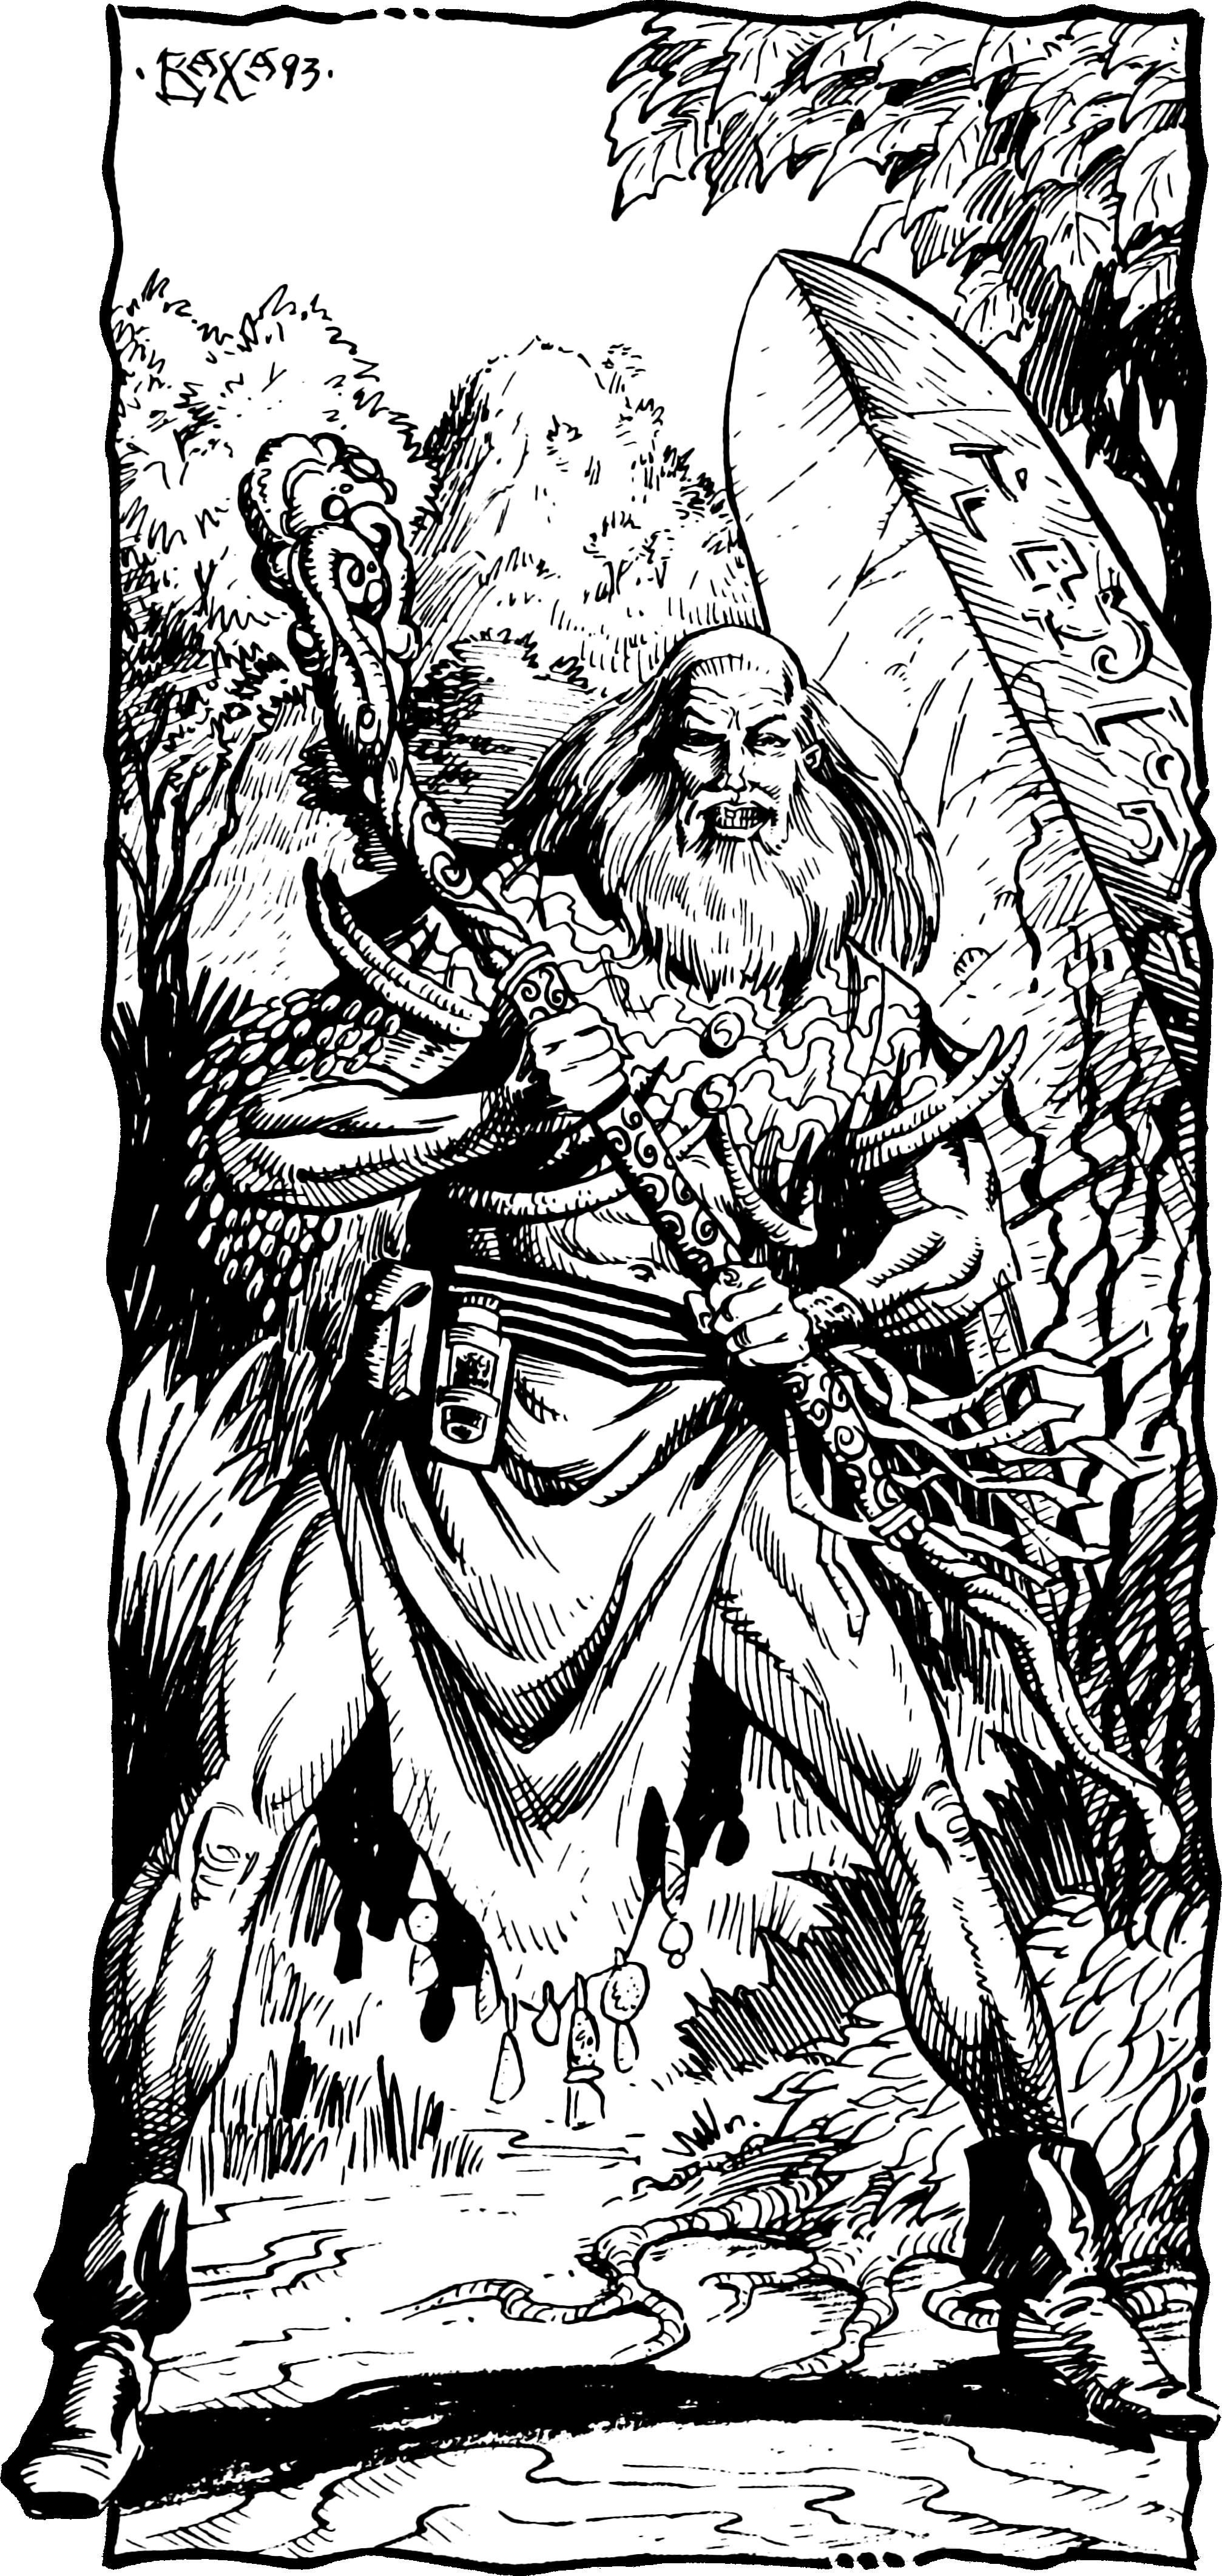
\includegraphics[width=\columnwidth]{images/druid-2.png}
\WOTC
\end{figure}

\subsubsection{Class Features}

\textbf{Weapon and Armor Proficiency:} Druids are proficient with the following weapons: alak, blowgun, club, dagger, dart, quarterstaff, scimitar, sickle, shortspear, sling, and spear. They are also proficient with all natural attacks (claw, bite, and so forth) of any form they assume with wild shape.

Druids are proficient with light and medium armor but are prohibited from wearing metal armor; thus, they may wear only padded, leather, or hide armor. (A druid may also wear wooden armor that has been altered by the ironwood spell so that it functions as though it were steel. See the ironwood spell description) Druids are proficient with shields (except tower shields) but must use only wooden ones.

A druid who wears prohibited armor or carries a prohibited shield is unable to cast druid spells or use any of her supernatural or spell-like class abilities while doing so and for 24 hours thereafter.

\textbf{Spells:} A druid casts divine spells, which are drawn from the druid spell list. Her alignment may restrict her from casting certain spells opposed to her moral or ethical beliefs; see Chaotic, Evil, Good, and Lawful Spells, below. A druid must choose and prepare her spells in advance (see below).

To prepare or cast a spell, the druid must have a Wisdom score equal to at least 10 + the spell level. The Difficulty Class for a saving throw against a druid's spell is 10 + the spell level + the druid's Wisdom modifier.

Like other spellcasters, a druid can cast only a certain number of spells of each spell level per day. Her base daily spell allotment is given on \tabref{The Druid}. In addition, she receives bonus spells per day if she has a high Wisdom score. She does not have access to any domain spells or granted powers, as a cleric does.

A druid prepares and casts spells the way a cleric does, though she cannot lose a prepared spell to cast a cure spell in its place (but see Spontaneous Casting, below). A druid may prepare and cast any spell on the druid spell list, provided that she can cast spells of  that level, but she must choose which spells to prepare during her daily meditation.

\textbf{Spontaneous Casting:} A druid can channel stored spell energy into summoning spells that she hasn't prepared ahead of time. She can ``lose'' a prepared spell in order to cast any summon nature's ally spell of the same level or lower.

\textbf{Chaotic, Evil, Good, and Lawful Spells:} A druid can't cast spells of an alignment opposed to her own. Spells associated with particular alignments are indicated by the chaos, evil, good, and law descriptors in their spell descriptions.

\textbf{Bonus Languages:} A druid's bonus language options include Sylvan, the language of woodland creatures. This choice is in addition to the bonus languages available to the character because of her race.

A druid also knows Druidic, a secret language known only to druids, which she learns upon becoming a 1st-level druid. Druidic is a free language for a druid; that is, she knows it in addition to her regular allotment of languages and it doesn't take up a language slot. Druids are forbidden to teach this language to nondruids. Druidic has its own alphabet.

% \textbf{Animal Companion (Ex):} A druid may begin play with an animal companion selected from the following list: lesser boneclaw, carru, dire rat, eagle, erdlu, jankx, jhakar, kes'trekel, kivit, owl, snake (Small or Medium viper). If the DM's campaign takes place wholly or partly in a silt environment, the DM may add silt spawn to the druid's list of options. This animal is a loyal companion that accompanies the druid on her adventures as appropriate for its kind. 

% A 1st-level druid's companion is completely typical for its kind except as noted below. As a druid advances in level, the animal's power increases as shown on the table. If a druid releases her companion from service, she may gain a new one by performing a ceremony requiring 24 uninterrupted hours of prayer. This ceremony can also replace an animal companion that has perished.

% A druid of 4th level or higher may select from alternative lists of animals. Should she select an animal companion from one of these alternative lists, the creature gains abilities as if the character's druid level were lower than it actually is. Subtract the value indicated in the appropriate list header from the character's druid level and compare the result with the druid level entry on the table to determine the animal companion's powers. (If this adjustment would reduce the druid's effective level to 0 or lower, she can't have that animal as a companion.)

\textbf{Nature Sense (Ex):} A druid gains a +2 bonus on \skill{Knowledge} (nature) and \skill{Survival} checks.

\textbf{Wild Empathy (Ex):} A druid can improve the attitude of an animal. This ability functions just like a \skill{Diplomacy} check made to improve the attitude of a person. The druid rolls 1d20 and adds her druid level and her Charisma modifier to determine the wild empathy check result. The typical domestic animal has a starting attitude of indifferent, while wild animals are usually unfriendly.

To use wild empathy, the druid and the animal must be able to study each other, which means that they must be within 9 meters of one another under normal conditions. Generally, influencing an animal in this way takes 1 minute but, as with influencing people, it might take more or less time.

A druid can also use this ability to influence a magical beast with an Intelligence score of 1 or 2, but she takes a $-4$ penalty on the check.

\textbf{Woodland Stride (Ex):} Starting at 2nd level, a druid may move through any sort of undergrowth (such as natural thorns, briars, overgrown areas, and similar terrain) at her normal speed and without taking damage or suffering any other impairment. However, thorns, briars, and overgrown areas that have been magically manipulated to impede motion still affect her.

\textbf{Trackless Step (Ex):} Starting at 3rd level, a druid leaves no trail in natural surroundings and cannot be tracked. She may choose to leave a trail if so desired.

\textbf{Nature's Speech (Su):} Starting at 4th level, a druid become able to speak with animals everywhere, as if under the effects of the \spell{speak with animals} spell.

\textbf{Wild Shape (Su):} At 5th level, a druid gains the ability to turn herself into any Small or Medium animal and back again once per day. Her options for new forms include all creatures with the animal type. This ability functions like the alternate form special ability, except as noted here. The effect lasts for 1 hour per druid level, or until she changes back. Changing form (to animal or back) is a standard action and doesn't provoke an attack of opportunity. Each time you use wild shape, you regain lost hit points as if you had rested for a night.

Any gear worn or carried by the druid melds into the new form and becomes nonfunctional. When the druid reverts to her true form, any objects previously melded into the new form reappear in the same location on her body that they previously occupied and are once again functional. Any new items worn in the assumed form fall off and land at the druid's feet.

The form chosen must be that of an animal the druid is familiar with.

A druid loses her ability to speak while in animal form because she is limited to the sounds that a normal, untrained animal can make, but she can communicate normally with other animals of the same general grouping as her new form. (The normal sound a wild parrot makes is a squawk, so changing to this form does not permit speech.)

A druid can use this ability more times per day at 6th and every three levels thereafter (9th, 12th, 15th, and 18th level). In addition, she gains the ability to take the shape of a Large animal at 9th level, a Tiny animal at 13th level, and a Huge animal at 17th level. The new form's Hit Dice can't exceed the character's druid level.

At 12th level, a druid becomes able to use wild shape to change into a plant creature with the same size restrictions as for animal forms. (A druid can't use this ability to take the form of a plant that isn't a creature.)

At 18th level, a druid becomes able to use wild shape to change into a vermin with the same size restriction as for animal forms. This transformation uses two wild shape daily uses. In addition to the normal effects of wild shape, the druid gains all the vermin's special qualities. (A druid maintains her Intelligence score and does not gain the vermin traits.)

% At 18th level, a druid becomes able to use wild shape to change into an elemental (air, earth, fire, or water) with the same size restriction as for animal forms. This transformation uses two wild shape daily uses. In addition to the normal effects of wild shape, the druid gains all the elemental's extraordinary, supernatural, and spell-like abilities. She also gains the elemental's feats for as long as she maintains the wild shape, but she retains her own creature type.

% At 18th level, a druid becomes able to assume elemental form twice per day, and at 20th level she can do so three times per day. At 20th level, a druid may use this wild shape ability to change into a Huge elemental.

\textbf{Venom Immunity (Ex):} At 8th level, a druid gains immunity to all poisons.

\textbf{A Thousand Faces (Su):} At 14th level, a druid gains the ability to change her appearance at will, as if using the \spell{disguise self} spell, but only while in her normal form. This affects the druid's body but not her possessions. It is not an illusory effect, but a minor physical alteration of the druid's appearance, within the limits described for the spell.

\textbf{Timeless Body (Ex):} After attaining 16th level, a druid no longer takes ability score penalties for aging and cannot be magically aged. Any penalties she may have already incurred, however, remain in place. Bonuses still accrue, and the druid still dies of old age when her time is up.

\subsubsection{Ex-Druids}
A druid who ceases to revere nature, changes to a prohibited alignment, or teaches the Druidic language to a nondruid loses all spells and druid abilities (not including weapon, armor, and shield proficiencies). She cannot thereafter gain levels as a druid until she atones (see the \spell{atonement} spell description).
% A druid who ceases to revere nature, changes to a prohibited alignment, or teaches the Druidic language to a nondruid loses all spells and druid abilities (including her animal companion, but not including weapon, armor, and shield proficiencies). She cannot thereafter gain levels as a druid until she atones (see the \spell{atonement} spell description).

% \subsubsection{The Druid's Animal Companion}
% A druid's animal companion is different from a normal animal of its kind in many ways. A druid's animal companion is superior to a normal animal of its kind and has special powers, as described below.

% \begin{figure}[b!]
% \centering
% 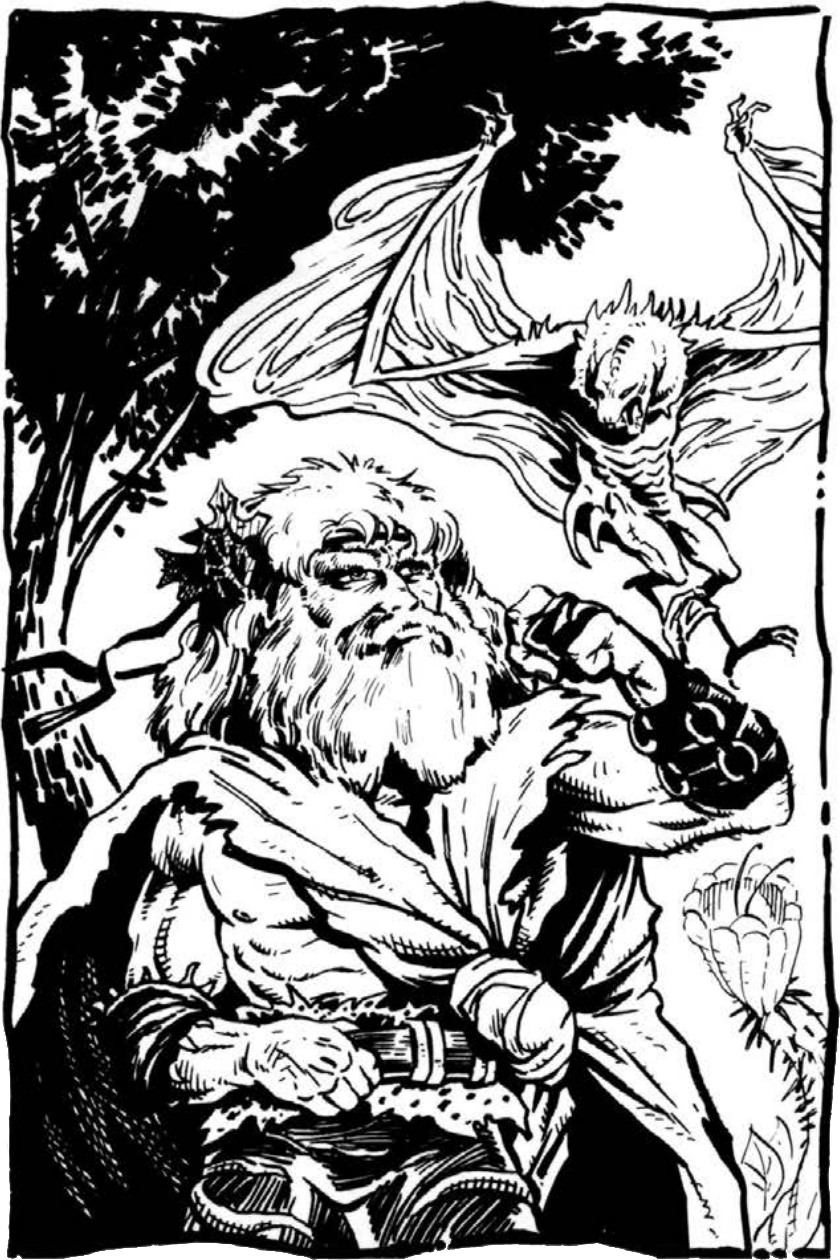
\includegraphics[width=\columnwidth]{images/druid-1.png}
% \WOTC
% \end{figure}

% \Table{}{l Z{.5cm} Z{.8cm} Z{.8cm} Z{.7cm} X}{\tableheader Class Level & \tableheader Bonus HD & \tableheader Natural Armor Adj. &\tableheader  Str/Dex Adj. &\tableheader  Bonus Tricks &\tableheader  Special\\
% 1st--2nd &&&& 1 & Link, share spells\\
% 3rd--5th & +2 & +2 & +1 & 2 & Evasion\\
% 6th--8th & +4 & +4 & +2 & 3 & Devotion\\
% 9th--11th & +6 & +6 & +3 & 4 & Multiattack\\
% 12th--14th & +8 & +8 & +4 & 5 &\\
% 15th--17th & +10 & +10 & +5 & 6 & Improved evasion\\
% 18th--20th & +12 & +12 & +6 & 7 &}

% \textbf{Animal Companion Basics:} Use the base statistics for a creature of the companion's kind, but make the following changes.

% \textbf{Class Level:} The character's druid level. The druid's class levels stack with levels of any other classes that are entitled to an animal companion for the purpose of determining the companion's abilities and the alternative lists available to the character.

% \textbf{Bonus HD:} Extra eight-sided (d8) Hit Dice, each of which gains a Constitution modifier, as normal. Remember that extra Hit Dice improve the animal companion's base attack and base save bonuses. An animal companion's base attack bonus is the same as that of a druid of a level equal to the animal's HD. An animal companion has good Fortitude and Reflex saves (treat it as a character whose level equals the animal's HD). An animal companion gains additional skill points and feats for bonus HD as normal for advancing a monster's Hit Dice.

% \textbf{Natural Armor Adj.:} The number noted here is an improvement to the animal companion's existing natural armor bonus.

% \textbf{Str/Dex Adj.:} Add this value to the animal companion's Strength and Dexterity scores.

% \textbf{Bonus Tricks:} The value given in this column is the total number of ``bonus'' tricks that the animal knows in addition to any that the druid might choose to teach it (see the \skill{Handle Animal} skill). These bonus tricks don't require any training time or \skill{Handle Animal} checks, and they don't count against the normal limit of tricks known by the animal. The druid selects these bonus tricks, and once selected, they can't be changed.

% \textbf{Link (Ex):} A druid can handle her animal companion as a free action, or push it as a move action, even if she doesn't have any ranks in the \skill{Handle Animal} skill. The druid gains a +4 circumstance bonus on all wild empathy checks and \skill{Handle Animal} checks made regarding an animal companion.

% \textbf{Share Spells (Ex):} At the druid's option, she may have any spell (but not any spell-like ability) she casts upon herself also affect her animal companion. The animal companion must be within 1.5 meter of her at the time of casting to receive the benefit. If the spell or effect has a duration other than instantaneous, it stops affecting the animal companion if the companion moves farther than 1.5 meter away and will not affect the animal again, even if it returns to the druid before the duration expires.

% Additionally, the druid may cast a spell with a target of ``You'' on her animal companion (as a touch range spell) instead of on herself. A druid and her animal companion can share spells even if the spells normally do not affect creatures of the companion's type (animal).

% \textbf{Evasion (Ex):} If an animal companion is subjected to an attack that normally allows a Reflex saving throw for half damage, it takes no damage if it makes a successful saving throw.

% \textbf{Devotion (Ex):} An animal companion gains a +4 morale bonus on Will saves against enchantment spells and effects.

% \textbf{Multiattack:} An animal companion gains \feat{Multiattack} as a bonus feat if it has three or more natural attacks and does not already have that feat. If it does not have the requisite three or more natural attacks, the animal companion instead gains a second attack with its primary natural weapon, albeit at a $-5$ penalty.

% \textbf{Improved Evasion (Ex):} When subjected to an attack that normally allows a Reflex saving throw for half damage, an animal companion takes no damage if it makes a successful saving throw and only half damage if the saving throw fails.

% \subsubsection{Alternative Animal Companions}
% A druid of sufficiently high level can select her animal companion from one of the following lists, applying the indicated adjustment to the druid's level (in parentheses) for purposes of determining the companion's characteristics and special abilities.

% Some animals are only available in certain environments. The animals available only in an aquatic environment, such as the Last Sea, are marked with $\dagger$. The animals available only in a silt environment, such as the Sea of Silt, are marked with $\diamond$.

% \Table{}{X X}{
% \multicolumn{2}{c}{\tableheader\footnotesize 4th Level or Higher (Level $-3$)}\\
% Carru, bull (6HD) & Leopard \\
% Cheetah & Lizard, giant \\
% Crodlu & Lizard, monitor\\
% Crodlu, heavy & Rasclinn\\
% Dire bat & Athasian shark$^\dagger$\\
% Erdland & Snake, constrictor\\
% Jhakar, Medium (6HD) & Snake, viper (Large)\\
% Kluzd & }

% \Table{}{X X}{
% \multicolumn{2}{c}{\tableheader\footnotesize 7th Level or Higher (Level $-6$)}\\
% Crodlu, heavy warmount & Puddingfish$^\dagger$ \\
% Inix & Lion\\
% Kalin & Lizard, subterranean\\
% Kluzd (7HD) & Snake, viper (Huge)\\
% Lirr & Takis\\
% Pterrax & Tiger}

% \Table{}{X X}{
% \multicolumn{2}{c}{\tableheader\footnotesize 10th Level or Higher (Level $-9$)}\\
% Cha'thrang & Lizard, minotaur\\
% Dire lion & Athasian shark (Huge)$^\dagger$ \\
% Hatori & Snake, giant constrictor}

% \Table{}{X X}{
% \multicolumn{2}{c}{\tableheader\footnotesize 13th Level or Higher (Level $-12$)}\\
% Lirr, large (11HD) & Athasian sloth\\
% Ruktoi$^\diamond$ & }

% \Table{}{X X}{
% \multicolumn{2}{c}{\tableheader\footnotesize 16th Level or Higher (Level $-15$)}\\
% Dire Athasian shark$^\dagger$ & Silt Horror, white$^\diamond$\\
% Dire tiger&Slimahacc\\
% Hatori, gargantuan (17HD) &}

\subsection{Playing a Druid}
You are a humanoid servant devoted to Athas and all of its elements equally. As a guardian, tender, warrior, and sometimes assassin, you further the cause of nature and help to make Athas verdant again.

You, like nature itself is neutral. You see the balance of all things. You know that every living creature is part of the food chain, and birth and death are the natural order of life. This is one of the reasons druids harbor such intense hatred for the defilers. Their magic of decay lies outside the normal cycle of life. Matter should not be destroyed, but converted to a form that will eventually return to the earth. Defiling magic destroys that which should never be destroyed, and its practice is an abomination to druids.

\subsubsection{Religion}
A druid is an individual who has devoted themselves to the balance of nature on Athas, and in particular someone who has sought out or been chosen by one of the few living spirits left in the barren land, protecting and nurturing them and the natural balance they represent.

Individual druids do not necessarily recognize one another as kin or as brothers in a religion; each conducts their affairs as they see fit in their quest to restore the balance of nature and protect their spirit's lands. Most druids recognize the various spirits as a manifestation of Athas itself, though some few more primitive or uncultured individuals or groups may believe the spirit to be a god and treat it as such.

\subsubsection{Other Classes}
Druids get along with most classes, though they despise wizards. Magic is the cause of Athas' current state, so say the druids, and while they may tolerate preservers for a short while, defilers are slain on sight. Templars are usually not welcomed by druids, as the templar is responsible for a city that encroaches on nature, and templars serve the sorcerer-kings, Athas' most powerful magic users. Elemental clerics are well received by druids, as they often share the same goals. Druids are usually at odds with paraelemental clerics, though. The paraelement proliferation on Athas is usually at the land's expense, destroying what the druid tries to accomplish.

Rangers are probably the druid's best allies. They often share the same goals, and the druid may even call upon the ranger for help in controlling a species that has become problematic or detrimental to an area. However, the ranger and the druid may sometimes be at odds, if the ranger is determined to eradicate his favored enemy while the druid seeks to protect that particular species.

\subsubsection{Combat}
Your ability to summon creatures and to turn into them is your primary weapons. Consider using them to aid your companions in flanking maneuvers, or better yet to harass enemy spellcasters (many of whom are easy to hit), especially if they are defilers. Few foes are prepared for an opponent who can call such potent beings to service, so you've also got the advantage of surprise.

Though somewhat skilled at both combat and spellcasting, you are more suited to guerrilla warfare---tracking enemies to their lair ambushing them while they sleep, or engaging in other sue surreptitious tactics. With woodland stride and trackless step, you can usually escape through the wilderness before your enemies know what hit them.

\subsubsection{Advancement}

You profit most from remaining a druid thought your advancement, so that %your animal companion and 
wild shape continue to improve as you gain levels. If you do multiclass, a level of barbarian is an excellent choice; the benefits it grants to combat and movement regardless of when you take that 1st level.

During their time of wandering, a young druid learns about the world, its ecology, the balance of nature and the ways of its creatures. After a few years of peregrination, most druids decide to settle in order to watch over a specific patch of land lands, watching over them and protecting them, and straighten their bond with a Spirit of the Land. Such druids become \class{Grove Masters}.

\subsection{Starting Packages}
\subsubsection{The Beastmaster}

Half-Elf Druid

\textbf{Ability Scores:} Str 10, Dex 15, Con 12, Int 8, Wis 15, Cha 12.

\textbf{Skills:} \skill{Handle Animal}, \skill{Hide}, \skill{Survival}.

\textbf{Languages:} Common, Elven.

\textbf{Feat:} \feat{Animal Affinity}.

\textbf{Weapons:} Longspear (1d8/$\times$3)

Sling with 20 bullets (1d4, 15 m).

\textbf{Armor:} Hide (+3 AC).

\textbf{Gear:} Spell component pouch, standard adventurer's kit, 20 cp.

\textbf{Class Features:} Jankx animal companion.

\textbf{Spells Prepared:} 1st---\spell{cure light wounds}, \spell{speak with animals}; 0---\spell{cure minor wounds} (2), \spell{defiler scent}.

\subsubsection{The Defiler Hunter}

Human Druid

\textbf{Ability Scores:} Str 13, Dex 14, Con 12, Int 10, Wis 15, Cha 8.

\textbf{Skills:} \skill{Concentration}, \skill{Hide}, \skill{Listen}, \skill{Move Silently}, \skill{Spot}, \skill{Survival}.

\textbf{Languages:} Common

\textbf{Feat:} \feat{Defender of the Land}, \feat{Track}.

\textbf{Weapons:} Spear (1d8/$\times$3, 6m)

Sling with 20 bullets (1d4, 15 m).

\textbf{Armor:} Hide (+3 AC).

\textbf{Gear:} Spell component pouch, standard adventurer's kit, 20 cp.

\textbf{Class Features:} Jhakar animal companion.

\textbf{Spells Prepared:} 1st---\spell{backlash}, \spell{longstrider};\hskip10pt 0---\spell{cure minor wounds}, \spell{defiler scent} (2).

\subsubsection{The Warden}

Pterran Druid

\textbf{Ability Scores:} Str 8, Dex 11, Con 14, Int 10, Wis 17, Cha 14.

\textbf{Skills:} \skill{Hide}, \skill{Knowledge} (nature), \skill{Move Silently}, \skill{Spot}, \skill{Survival}.

\textbf{Languages:} Saurian.

\textbf{Feat:} \feat{Spell Focus} (conjuration).

\textbf{Weapons:} Alak (1d6/$\times$3)

Blowgun with 20 needles (1, 3 m).

\textbf{Armor:} Leather (+2 AC), light wooden shield (+1 AC).

\textbf{Gear:} Spell component pouch, standard adventurer's kit, 20 cp.

\textbf{Class Features:} Lesser boneclaw animal companion.

\textbf{Spells Prepared:} 1st---\spell{entangle}, \spell{plant renewal}; 0---\spell{defiler scent}, \spell{detect magic}, \spell{nurturing seeds}.

\subsection{Druids on Athas}
\Quote{The druids are no longer hunted in force by the sorcerer-kings. The kings believe there simply aren't enough left to threaten them. But the templars, and even some elves I know, have been well rewarded for delivering the heads of wasteland druids.}{Jurgan, Urikite earth cleric}

Perhaps the only thing rarer to see in Athas than a wizard is a druid. After centuries of persecution, they were forced to either die in the hands of the agents of the sorcerer-monarchs, or to watch their beloved land wither and die before their eyes.

Because of that, druids are usually loners and avert to social interaction. They live off the land, within the land, and they have sacrificed their entire lives for the land, very little besides it occupies the mind of a druid.

\subsubsection{Daily Life}

A druid adventures to learn about Athas, to protect nature, and to further his own aims. Druids usually spend their days in contemplation of nature, and tending their lands; one may watch over a particular stretch of open desert, another may protect a belt of scrub grass within it, while still another might watch over a small oasis that borders on both, always hidden and always watching.

The Athasian druid is a wanderer who hunts down a powerful defiler that has despoiled the wastes, or a visionary who tends the land and teaches the local population how to live in harmony with their surroundings. The Athasian druid fights for an almost lost cause, and it matters not if that cause is revenge himself against those who destroyed his land and friends or a ceaseless desire to bring green and hope to Athas.

\subsubsection{Notables}

Druids very rarely become famous, since they usually avoid social interaction combined the fact that it might put their lives at risk since usually sorcerer-kings and defiler usually put a reward for the head of a notorious or troublesome druid. A legend claim that Mearedes the druidess came to the island of Shault when its forest was all but dead and she managed to nurture it back to its vibrant health.

\subsubsection{Organizations}

Ever since the Eradication, an anti-druidic jihad led by sorcerer-kings more than 1,500 years ago, no specific druidic organization exists, although some form temporary alliances with Veiled Alliance members from time to time. Legends say that the druids who remained after the Eradication gathered on a high mesa somewhere in the northern Tablelands. It was there they decided that they should scatter to the most remote reaches and farthest regions of Athas, there to bide their time, waiting for the day when they were powerful enough to challenge the sorcerer-kings again. This was a long time ago, and the druids have yet to return to the cities of the defilers. Some say that they will never return and that their seclusion and isolation have destroyed whatever power they once wielded as a circle. Others say that the druid's long wait is indicative of their cunning, and that their plan is to insure that the next confrontation with the kings won't end in defeat.

\subsubsection{NPC Reactions}

Druids are natural loners, and usually avoid social interactions unless they have to. In such cases, those who are directly benefited from the druid's work of tending the land begin two steps nearer helpful, while defilers and evil paraelemental clerics begin two steps nearer hostile.

\subsubsection{Druid Lore}

Characters with ranks in \skill{Knowledge} (nature) can research druids to learn more about them. When a character makes a skill check, read or paraphrase the following, including the information from lower DCs.

\textbf{DC 10:} Druids devote themselves to the land, drawing off their power straight from Athas itself.

\textbf{DC 15:} Druids from a mystical connection to mysterious beings known as Spirits of the Land. They hate all defilers and those who abuse the land.

\textbf{DC 20:} Druids are masters of the forces of nature, being able to transform into the creatures that dwell in their lands, and some even learn to counter the destruction of defilement.

\Class{Fighter}
{Any wastelander can pick up a bone and call it a club, but try pitting fifty of those against one dozen trained soldiers, and maybe you'll have an even match.}{Nikolos, human fighter}

From the small forts in sandy wastes of Athas to the guards of the merchant houses in the city-states, fighters are Athas' most common sight. Whether it is as mercenaries for the sorcerer-kings or as hired guards protecting the wealth of the nobility, fighters can be found everywhere in the Tablelands. Athas' fighters are trained to fight in small groups or huge units. Those that have proven themselves become the commanders in the city-states' armies, commanding hundreds or even thousands of men into war.

\subsection{Making a Fighter}
Fighters receive the best allotment of fighting skills and abilities. They learn the use of most weapons, the best armors and shields, as well as gaining special abilities to use with these weapons and armor.

Some fighters specialize in using a single weapon, and become masters at its use and deadliness. Other fighters will prefer more rounded skills, learning to shoot from far with bows and arrows, or nets or spears. Regardless, the fighter is to be feared.

\textbf{Races:} All of Athas' races can become fighters. Humans are usually the most numerous, though, since they are the most numerous of the races of the Tablelands. Dwarves make good fighters, even though they are smaller than most races; their inborn toughness and great strength more than makes up for their smaller stature. The half-giants are also seen very often as fighters, since their great strength and size are perfect for the job. Muls, with the inherited traits of both humans and dwarves, are also great fighters. Elves, with their long legs and frail constitution, are not often seen as fighters. Athas' intelligent insects, the Thri-kreen, make excellent warriors, with their four arms and the fact they do not need to sleep. Many of the savage races of the Tablelands are fighters, although most become rangers in order to survive.

\textbf{Alignment:} Fighters come from all walks of life, and can be of any alignment. Good fighters are usually seen as the protectors of small villagers or are part of renegade slave tribes, helping their tribe to survive in the harsh desert. Or they can be found as a dwarf perhaps, whose focus it is to guard his fellows. Evil fighters are often part of mercenary bands or under the control of a sorcerer-king; these beings often fight for power and money. Evil fighters can also be found as the rulers of small forts, guarding their oasis and exacting a hefty toll for its use.

\Figure{t}{images/fighter-3.png}

\MiniWarriorTable{The Fighter}{
1st  & +1             & +2  & +0 & +0 & Bonus feat \\
2nd  & +2             & +3  & +0 & +0 & Bonus feat \\
3rd  & +3             & +3  & +1 & +1 &  \\
4th  & +4             & +4  & +1 & +1 & Bonus feat \\
5th  & +5             & +4  & +1 & +1 & Martial prowess \\
6th  & +6/+1          & +5  & +2 & +2 & Bonus feat \\
7th  & +7/+2          & +5  & +2 & +2 & Martial prowess \\
8th  & +8/+3          & +6  & +2 & +2 & Bonus feat \\
9th  & +9/+4          & +6  & +3 & +3 & Martial prowess \\
10th & +10/+5         & +7  & +3 & +3 & Bonus feat \\
11th & +11/+6/+1      & +7  & +3 & +3 & Martial prowess \\
12th & +12/+7/+2      & +8  & +4 & +4 & Bonus feat \\
13th & +13/+8/+3      & +8  & +4 & +4 & Martial prowess \\
14th & +14/+9/+4      & +9  & +4 & +4 & Bonus feat \\
15th & +15/+10/+5     & +9  & +5 & +5 & Martial prowess \\
16th & +16/+11/+6/+1  & +10 & +5 & +5 & Bonus feat \\
17th & +17/+12/+7/+2  & +10 & +5 & +5 & Martial prowess \\
18th & +18/+13/+8/+3  & +11 & +6 & +6 & Bonus feat \\
19th & +19/+14/+9/+4  & +11 & +6 & +6 & Martial prowess \\
20th & +20/+15/+10/+5 & +12 & +6 & +6 & Bonus feat \\
}

\subsection{Game Rule Information}
\textbf{Hit Die:} d10.

\subsubsection{Class Skills}
\skill{Autohypnosis} (Wis), \skill{Climb} (Str), \skill{Craft} (Int), \skill{Handle Animal} (Cha), \skill{Intimidate} (Cha), \skill{Jump} (Str), \skill{Knowledge} (warcraft) (Int), \skill{Ride} (Dex), and \skill{Spot} (Wis).

\textbf{Skill Points per Level:} 4 + Int modifier ($\times4$ at 1st level).

\subsubsection{Class Features}
\textbf{Weapon and Armor Proficiency:} A fighter is proficient with all simple and martial weapons and with all armor (heavy, medium, and light) and shields (including tower shields).

\textbf{Bonus Feats:} At 1st level, a fighter gets a bonus combat-oriented feat in addition to the feat that any 1st-level character gets and the bonus feat granted to a human character. The fighter gains an additional bonus feat at 2nd level and every two fighter levels thereafter (4th, 6th, 8th, 10th, 12th, 14th, 16th, 18th, and 20th). These bonus feats must be drawn from the feats noted as fighter bonus feats. A fighter must still meet all prerequisites for a bonus feat, including ability score and base attack bonus minimums.

These bonus feats are in addition to the feat that a character of any class gets from advancing levels. A fighter is not limited to the list of fighter bonus feats when choosing these feats.

\textbf{Martial Prowess:} At 5th level and every two levels thereafter, a fighter improves his repertoire with new techniques. He may choose one of the following options.

\textit{Active Defense (Ex):} A fighter gains a dodge bonus to AC equal to \onequarter his fighter levels when wielding a shield and fighting defensively or using the \feat{Combat Expertise} feat. When using total defense, this bonus increases to \onehalf his fighter levels.

\textit{Aim (Ex):} A fighter can take full-round action to make a \skill{Spot} check to improve his next attack against a specific foe. DC is equal to his target's AC. His next attack against the target ignore armor bonus and natural armor bonus. This attack must be made within a number of rounds equal to \onequarter his fighter levels.

\Figure*{t}{images/battle-1.png}

\textit{Ambidextrous (Ex):} A fighter may add his full Strength modifier to his off-hand weapon damage, instead of \onehalf his Strength bonus.

\textit{Bravery (Ex):} A fighter with this ability gains a bonus equal to \onehalf his fighter levels on Will saves against mind-affecting abilities.

\textit{Close Combat Shot (Ex):} A fighter can attack with a ranged weapon while in a threatened square and not provoke an attack of opportunity.

\textit{Commanding Strike (Ex):} A fighter may forgo his attack with the lowest base attack bonus in a total attack to create an opening for an ally. The designated ally may use one of his attacks of opportunity to strike a foe. The ally may use ranged attacks---this is an exception for the rules for attacks of opportunity.

\textit{Coordinate Allies (Ex):} A fighter can use a full-round action to identify and apply an effective tactic for his allies. Each creature to be affected must be able to see and hear him, and able to pay attention to him. To coordinate, the fighter must make a \skill{Knowledge} (warcraft) check with a DC equal to 15 + the number of allies affected. If the check succeeds, all affected allies gain a competence bonus on attack rolls or a dodge bonus to AC equal to \onequarter his fighter levels. He chooses which of the two benefits to impart and must impart the same benefit to all affected allies. The benefits last for 1 round. The fighter cannot use this ability on himself.

\textit{Crossbowman (Ex):} Whenever a fighter attacks with a crossbow as a readied action, his target is denied its Dexterity bonus to its AC.

\textit{Defensive Tactics (Ex):} A fighter may use a move action to coordinate his allies to a defensive maneuver. Each creature to be affected must be able to see and hear him, and able to pay attention to him. To coordinate, the fighter must make a \skill{Knowledge} (warcraft) check with a DC equal to 10 + the number of allies affected. If the check succeeds, all affected allies gain a moral bonus to AC against attacks of opportunity equal to \onequarter his fighter levels. The benefits last for 1 round.

\textit{Double Opportunity (Ex):} When a fighter makes an attack of opportunity, he may attack once with both his primary and secondary weapons. The penalties for attacking with two weapons apply normally. The fighter must be at least 11th level to select this technique.

\textit{Flanking Tactics (Ex):} A fighter may use a move action to coordinate his allies to a flanking maneuver against a target. Each creature to be affected must be able to see and hear him, and able to pay attention to him. To coordinate, the fighter must make a \skill{Knowledge} (warcraft) check with a DC equal to the target's Base Attack Bonus. If the check succeeds, all affected allies gain a competence bonus on damage rolls equal to \onequarter his fighter levels when they flank the target. The benefits last for 1 round. The fighter cannot use this ability on himself.

\textit{Harden Resolve (Ex):} A fighter may use a standard action to improve his allies' morale. Each creature to be affected must be able to see and hear him, and able to pay attention to him. To coordinate, the fighter must make a \skill{Knowledge} (warcraft) check with a DC equal to 25 + 2 for each ally affected. If the check succeeds, all affected allies gain damage reduction equal to \onequarter his fighter levels. If an ally already has damage reduction, it improves by the same amount. The benefits last for 1 round. A fighter must be at least 11th level to select this technique.

\textit{Hawkeye (Ex):} Whenever a fighter isn't flat-footed, he has advantage on \skill{Spot} checks.

\textit{Lead the Charge (Ex):} A fighter may make a \skill{Knowledge} (warcraft) check during a charge against one specific foe. The check DC is equal to 20 + the number of allies affected. If the check succeeds, all affected allies that charge the same foe gain a competence bonus on attack and damage rolls equal to \onequarter his fighter levels. The benefits last for 1 round.

\textit{Leadership:} A fighter may gain the \feat{Leadership} feat as a bonus feat.

\textit{Maneuvering Attack (Ex):} A fighter may forgo his attack with the lowest base attack bonus in a total attack to maneuver one of his comrades into a more advantageous position. The fighter chooses a friendly creature that can see and hear him. That creature can use an immediate action to move up to half its speed.

\textit{Martial Versatility (Ex):} A fighter can apply any feat he has that affects only one weapon type (such as, \feat{Weapon Focus} or \feat{Rapid Reload}) to any simple weapon. A fighter must be at least 11th level to select this technique.

\textit{Mirror Move (Ex):} A fighter gains \onequarter his fighter levels as an insight bonus to AC when attacked by any weapon with which he has the \feat{Weapon Specialization} feat.

\textit{Overhand Chop (Ex):} When a fighter makes a single attack (with the attack action or a charge) with a two-handed weapon, he adds triple his Strength bonus on damage rolls, instead of 1\onehalf his Strength bonus.

\textit{Phalanx (Ex):} As long as a fighter is wielding a shield, he may use any two-handed polearm or spear as if it was an one-handed weapon. A fighter cannot use this ability with a buckler.

\textit{Pressing Shield (Ex):} A fighter may use his shield to help with his bull rush and overrun attempts. He adds his shield bonus on Strength checks made to push back the defender, and on Strength checks to knock down his opponent. A fighter cannot use this ability with a buckler.

\textit{Quick Aid (Ex):} A fighter may use the aid another action with a full attack. He must use his attack with the highest base attack bonus and roll against AC 20.

\textit{Ready Polearm (Ex):} A fighter can ready any weapon that deals increased damage against charge as an immediate action. A fighter must be at least 11th level to select this technique.

\textit{Second Wind (Ex):} A fighter with this ability can dig his resolve and endurance to find an extra burst of vitality. He can use a standard action to gain a number of temporary hit points equal to his Constitution modifier $\times$ his fighter levels. These hit points last until for the end of the encounter. He can use this ability only once per encounter.

\textit{Shield Another (Ex):} A fighter can use his shield to protect an adjacent ally. When using aid another to grant AC to an ally, he can choose a number to add as penalty to his shield bonus until his next turn. The ally target of the aid another action gains improves their shield bonus by that number. The fighter can't choose a number greater than his shield bonus or his base attack bonus. A fighter cannot use this ability with a buckler.

\textit{Shorten Haft (Ex):} A fighter may threaten adjacent squares when wielding reach weapons.

\textit{Skirmisher (Ex):} Whenever a fighter moves 3 or more meters in his turn, he gains a dodge bonus against ranged attacks equal to \onequarter his fighter.

\textit{Tortoise Style (Ex):} While wielding a shield, the fighter improves his shield bonus by \onequarter his fighter levels. A fighter cannot use this ability with a buckler.

\textit{Two-handed Style (Ex):} When the fighter rolls a 1 or 2 on a damage die for an attack made with a melee weapon wielded with two hands, he can reroll the die and must use the new roll even if the new roll is a 1 or 2. The fighter cannot use this benefit with light weapons.

\textit{Uncanny Dodge (Ex):} A fighter can react to danger before his senses would normally allow his to do so. He retains his Dexterity bonus to AC (if any) even if he is caught flat-footed or struck by an invisible attacker. However, he still loses his Dexterity bonus to AC if immobilized. If a fighter already has uncanny dodge from a different class he automatically gains improved uncanny dodge instead.

\textit{Weapon Training (Ex):} A fighter improves his aptitude in martial weapons. He gains a competence bonus on his attack rolls equal to \onequarter his fighter levels, whenever he is wielding a simple or martial weapon.


\subsection{Playing a Fighter}
Playing an Athasian fighter is not much different than playing one in other settings, the only difference is that the extreme heat makes most armor less than desirable on Athas.

As a fighter, you undertake adventures according to the dictates of your cause, your faith, or your own selfish needs. You might find yourself on the hot, sandy field of battle, charging shoulder to shoulder with peasants and soldiers, raising pitchforks and shields against the defilers of the enemy army.

\subsubsection{Religion}
There are no gods on Athas, but many fighters worship the sorcerer-king of their respective cities as gods. Some fighters pay homage to the elemental forces of the Tablelands, asking their favored element for luck before entering the battlefield.

\subsubsection{Other Classes}
Fighters get along with most other classes. The rangers of the Tablelands often receive the highest of the respect for their ability to survive the wastes. Gladiators and fighters are often at each other's throats, since both share great combat abilities but differ in their methodology; they often try to show how each is better than the other is. Elemental clerics are welcome for their healing abilities as well as the help they can provide in battle.

Fighters are uneasy around wizards; like the rest of the population they distrust magic. Templars are also distrusted, for the same reasons everyone else distrusts templars. Rogues are usually scorned by fighters; they prefer open battle to the rogue's sneaky ways.

\subsubsection{Combat}
Your specific tactics in battle depend on your role in the party and your weapon of choice. However, certain tactics are common to all fighters.

You are generally at the forefront of any battle. Fighting on the front line allows you maximize your combat feats. Furthermore, if opponents focus on you, they cannot injure your allies. As a fighter, you're at your best when you can take on the monster or opponent that deals the most damage.

\subsubsection{Advancement}
When looking at feats to select as you gain levels, you have two basic paths. You can focus on your fighting skills, or you can attempt to expand your capabilities to serve as the party's leader. The former option is best when you are the group's primary combat specialist. If the party includes another fighter or suitable melee character, you can afford to dabble in Charisma-based skills. Although Diplomacy is not a class skill for you, the Field Office feat combined with a few cross-class ranks makes you a serviceable emissary.

When it comes to combat feats, look to ones that improve your ability to deal damage. Feats such as Power Attack, Weapon Focus, and so forth are excellent options to boost your offense. Concentrated Fire, Rotate Lines, Shield Wall, and Spear Wall are excellent feats for army fighters.

Improved Initiative is a critically important feat, since it allows you to act first, move forward and defend or guide your allies. The sooner you find a place in the front line, the longer you can hold back the enemy.


\subsection{Starting Packages}
\subsubsection{The Archer}
Elf Fighter

\textbf{Ability Scores:} Str 15, Dex 16, Con 11, Int 10, Wis 12, Cha 8.

\textbf{Skills:} \skill{Jump}, \skill{Spot} (cc).

\textbf{Languages:} Common, Elven.

\textbf{Feat:} \feat{Point Blank Shot}, \feat{Precise Shot}.

\textbf{Weapons:} Macahuitl (1d8/19-20)

Dagger (1d4/19-20, 3 m)

Longbow with 40 arrows (1d8/$\times$3, 30 m).

\textbf{Armor:} Chitin armor (+4 AC).

\textbf{Gear:} Standard adventurer's kit, 11 cp.

\subsubsection{The Defender}
Dwarf Fighter

\textbf{Ability Scores:} Str 15, Dex 13, Con 16, Int 10, Wis 12, Cha 8.

\textbf{Skills:} \skill{Craft} (weaponsmithing), \skill{Knowledge} (warcraft), \skill{Intimidate}.

\textbf{Languages:} Common, Dwarven.

\textbf{Feat:} \feat{Disciplined}, \feat{Weapon Focus} (dwarven waraxe).

\textbf{Weapons:} Dwarven waraxe (1d10/$\times$3)

Shortbow with 20 arrows (1d6/$\times$3, 18 m).

\textbf{Armor:} Scale mail (+4 AC), heavy wooden shield (+2 AC).

\textbf{Gear:} Standard adventurer's kit, 42 cp.

\subsubsection{The Leader}
Human Fighter

\textbf{Ability Scores:} Str 15, Dex 8, Con 13, Int 10, Wis 12, Cha 14.

\textbf{Skills:} \skill{Diplomacy} (cc), \skill{Knowledge} (warcraft), \skill{Intimidate}.

\textbf{Languages:} Common.

\textbf{Feat:} \feat{Field Officer}, \feat{Inspiring Presence}, \feat{Weapon Focus} (great macahuitl).

\textbf{Weapons:} Great macahuitl (2d6, 19-20)

Shortbow with 20 arrows (1d6/$\times$3, 18).

\textbf{Armor:} Scale mail (+4 AC).

\textbf{Gear:} Standard adventurer's kit, 19 cp.


\subsection{Fighters on Athas}
\Quote[-.em]{Yeah, he was alright with a sword, but he would wet himself every time we walked out onto the sand of the arena. I think it was the crowd... or the goat-headed giant they paired us against. Poor little weed, he never saw that club coming.}{Grek the Grand, talking about his onetime matched pair contest with Slavek Thydor}

Fighters bring clashing weapons, stirring speeches, and mass combat to the campaign. On Athas, the fighter is a trained warrior, a soldier skilled in mass warfare. Every society on Athas maintains an army of fighters to protect itself from attack or to wage wars of plunder and annihilation against its neighbors. Fighters are both the commanders and soldiers in these armies, and at higher levels are experts in both individual and formation combat, leadership, and morale.

\subsubsection{Daily Life}
A fighter adventures to prove his superior skill at arms, to advance the cause of whatever master he might serve, and to further his own aims.

Once he has reached a respectable level of accomplishment, a fighter might take the Leadership feat and start building his own army. As word spreads, less experienced warriors who are eager to fight for the same causes seek him out as the desperate peoples of Athas constantly look for great commanders, warriors who will lead them.

\subsubsection{Notables}
Fighters can notoriety for their deeds, whether triumphs in combat, selfless acts of great honor, or great tyranny. Many an adventurer grew up on stories such as that of the Crimson Legion, and how it managed to defeat Urik's previously undefeated army.

Another legend tells of about the rise and fall of General Zanthiros, the leader of the Balican army who managed to save the city from an onslaught of beast-headed giants more than once, and after losing the elections, left the city with hundreds of soldiers loyal to him and formed a raiding tribe.

\subsubsection{Organizations}
Fighters often band together into small armies or as mercenary groups working for trade houses. These organizations typically have different credos and values, but they allow their members to focus their time on their individual quests.

\subsubsection{NPC Reactions}
Individuals react to fighters based on their previous interactions with other members of the class. A brave fighter meets cold silence and contempt around the Barrier Wastes where evil fighters oppress the populace.

Gladiators usually talk down on fighters, saying that gladiators are the true masters of combat. Fighters usually reply that gladiators are nothing without a crowd looking. Because of that, their initial reaction is one step towards unfriendly than normal.

A fighter who has lived long enough to retire from adventuring typically acquires some position of authority, with commensurate political power, whether as a caravan leader, army general, or ruler of a raiding or slave tribe.

\subsubsection{Fighter Lore}
Characters with ranks in \skill{Knowledge} (warcraft) can research fighters to learn more about them. When a character makes a skill check, read or paraphrase the following, including the information from lower DCs.

\textbf{DC 10:} Fighters may not be as flashy as gladiators in combat, but they surely are more effective in mass combat.

\textbf{DC 15:} Fighters are combat-oriented characters adept at hand-on-hand combat just as well as commanding entire armies.

\textbf{DC 20:} A fighter's mere presence in the battlefield can be enough to inspire his soldiers and weaken the resolve of his enemies.

\Class{Gladiator}
{I might be a slave, but I am famous, I dine well, and my company is that of the finest noble women. Tell me, what do you have that I do not, slave trader---except the freedom to feel miserable?}{Jarek, arena champion}

\begin{figure}[t!]
\centering
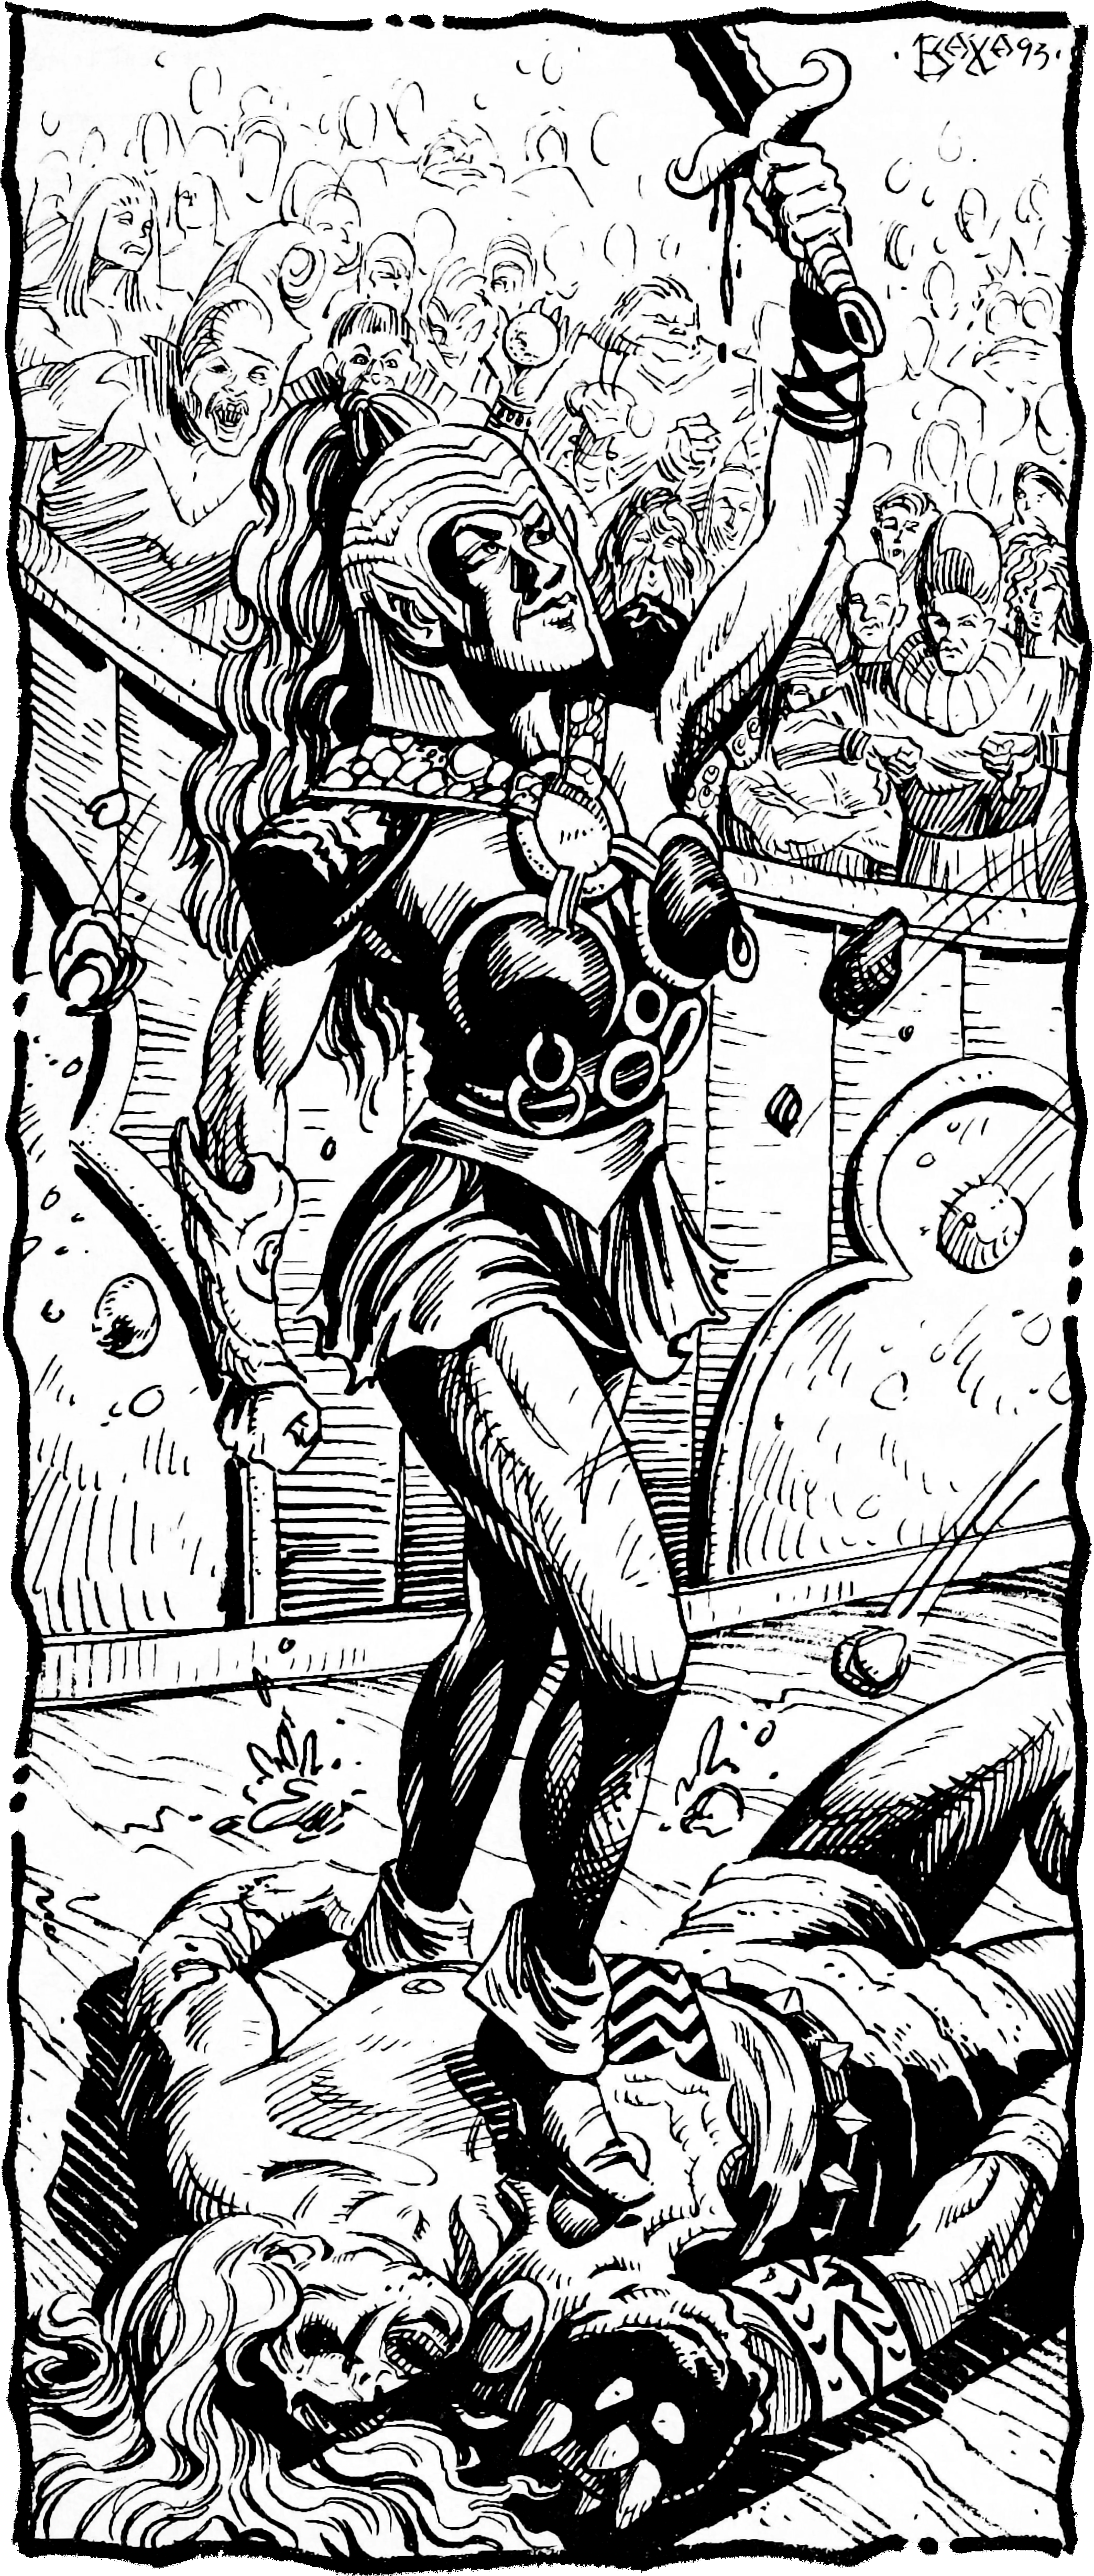
\includegraphics[width=\columnwidth]{images/gladiator-2.png}
\WOTC
\end{figure}

The arena is the battlefield of the gladiator. From hand-to-hand combat in the mud pits of small forts to the grand games of the city-states, the gladiator is a warrior who fights to the sounds of people cheering his name or cursing his presence. A master of crowd control and the art of prolonged combat, gladiators are trained to fight.

They train to best wild beasts in deadly games for the amusement of the masses. They fight for glory, wealth, prestige and power. They fight to survive. Some are merely slaves, having to fight and perhaps hoping to win a chance to obtain freedom, while some fight willingly for the thrill of combat or the promise of riches and fame.

\WarriorTable[ll *{3}{C} p{8cm}]{The Gladiator}{
1  & +1             & +2  & +0 & +0 & Unarmed strike, gladiatorial performance, dirty trick +1/$-1$                 \\
2  & +2             & +3  & +0 & +0 & Bonus feat, exotic weapon, stance (arena guile)                               \\
3  & +3             & +3  & +1 & +1 & Bonus feat, exotic aptitude, taunt                                            \\
4  & +4             & +4  & +1 & +1 & Uncanny dodge                                                                 \\
5  & +5             & +4  & +1 & +1 & Armor optimization 1, \feat{Improved Feint}                                   \\
6  & +6/+1          & +5  & +2 & +2 & Exotic weapon, parry, shake off                                               \\
7  & +7/+2          & +5  & +2 & +2 & Bonus feat, dirty trick +2/$-2$, stance (threatening glare, defensive stance) \\
8  & +8/+3          & +6  & +2 & +2 & Improved uncanny dodge, mercy                                                 \\
9  & +9/+4          & +6  & +3 & +3 & \feat{Leadership}, pounce                                                     \\
10 & +10/+5         & +7  & +3 & +3 & Armor optimization 2, exotic weapon                                           \\
11 & +11/+6/+1      & +7  & +3 & +3 & Improved parry                                                                \\
12 & +12/+7/+2      & +8  & +4 & +4 & Dragon's fury, stance (keen eye, scoundrel pose)                              \\
13 & +13/+8/+3      & +8  & +4 & +4 & Dirty trick +3/$-3$, greater feint                                            \\
14 & +14/+9/+4      & +9  & +4 & +4 & Exotic weapon                                                                 \\
15 & +15/+10/+5     & +9  & +5 & +5 & Armor optimization 3, dragon's speed                                          \\
16 & +16/+11/+6/+1  & +10 & +5 & +5 & Greater parry                                                                 \\
17 & +17/+12/+7/+2  & +10 & +5 & +5 & Stance (balancing dance, hypnotic fortitude)                                  \\
18 & +18/+13/+8/+3  & +11 & +6 & +6 & Exotic weapon, mindless focus                                                 \\
19 & +19/+14/+9/+4  & +11 & +6 & +6 & Dirty trick +4/$-4$                                                           \\
20 & +20/+15/+10/+5 & +12 & +6 & +6 & Armor optimization 4                                                          \\
}


\subsection{Making a Gladiator}
Gladiators are among the best one-on-one fighters in all the Tablelands. They are trained in hand-to-hand combat before moving on to the use of exotic weapons of the arena. They learn to improvise weapons, wielding broken bones or wooden shafts with deadly precision. They learn how to taunt and tease opponents, driving them to reckless acts and taking advantage of the situation to strike down or maim a foe.

After all, a long, drawn-out combat is more a crowd pleaser than a ten-second bout.

\textbf{Abilities:} Strength and Constitution are vital to a gladiator, since he is often in harm's way. Intelligence is useful for gaining plenty of skills points, which a gladiator needs to purchase Bluff, Intimidate, Performance, and Sense Motive, key skills for any arena performer.

\textbf{Races:} All races of Athas can be found in the arenas of the Tablelands. Muls, with their mixed dwarven and human parentage, are highly prized in the arenas. They are often bought for a high price and treated well in return for victory on the combat floor. Elves are often used for their swiftness and natural flair for taunting their opponent. Humans are the most common of gladiators, since humans are the most common race in the Tablelands. Halflings make poor gladiators, since they abhor slavery and will usually starve themselves to death rather than being used as commodities by anyone. The savage races of the wastes are often used as gladiators, usually as fodder for the most successful gladiators, though those demonstrating excellent combat prowess receive formal training.

\textbf{Alignment:} Gladiators are of all alignments. Some gladiators will obey all arena rules, being lawful individuals, though these often do not last long in the arena. Many gladiators tend toward a chaotic alignment. Evil gladiators use dirty tricks to gain an advantage over an opponent. Gladiators of all alignments can become crowd favorites, increasing their chances of winning their matches, since often times these matches are prearranged. The intrigues of the city-states can reach deep into the arena.

\subsection{Game Rule Information}

\textbf{Hit Die:} d8.

\subsubsection{Class Skills}
\skill{Autohypnosis} (Wis), \skill{Balance} (Dex), \skill{Bluff} (Cha), \skill{Climb} (Str), \skill{Craft} (Int), \skill{Handle Animal} (Cha), \skill{Intimidate} (Cha), \skill{Jump} (Str), \skill{Perform} (Cha), \skill{Profession} (Wis), \skill{Ride} (Dex), \skill{Sense Motive} (Wis), \skill{Spot} (Wis), and \skill{Tumble} (Dex).

\textbf{Skill Points per Level:} 4 + Int modifier ($\times4$ at 1st level).

\subsubsection{Class Features}

\textbf{Weapon and Armor Proficiency:} You are proficient with all simple and martial weapons, light armor, medium armor and shields (except tower shields).

\textbf{Gladiatorial Performance:} Once per day per gladiator level, you can use your talents to affect enemies and allies. Each ability requires both a minimum gladiator level and a minimum number of ranks in the \skill{Perform} (arena fighting) skill to qualify. Starting a gladiatorial performance effect is a move action unless otherwise stated.

\textit{Dirty Trick (Ex):} A gladiator with 3 or more ranks in \skill{Perform} (arena fighting) can use his arena guile to get an advantage over his enemies. Once per encounter per opponent, a gladiator can use a dirty trick to do one of the following:

\begin{itemize*}
\item Gain +1 morale bonus on his attack rolls for one round.
\item Gain +1 morale bonus on his damage rolls for one round.
\item Impose $-1$ morale penalty on target opponent's attack rolls for one round.
\item Impose $-1$ morale penalty on target opponent's damage rolls for one round.
\end{itemize*}

A gladiator can use dirty trick more than once per encounter, but a gladiator may never repeat the same option against the same enemy or use it more than once in a single round against the same enemy. Using a dirty trick is a free action.

The bonus and penalties increase by 1 at 7th level and every six levels thereafter (+2/$-2$ at 7th, +3/$-3$ at 13th, and +4/$-4$ at 19th).

\textit{Taunt (Ex):} A gladiator of 3rd level or higher with 6 or more ranks in \skill{Perform} (arena fighting) can taunt one opponent to fly into a rage. The opponent to be taunted must be within 9 meters, able to see and hear the gladiator, and must have an Intelligence of 3 or higher. The gladiator must also be able to see the creature. For every three levels a gladiator attains beyond the 1st, he can target one additional creature with a single use of this ability.

A gladiator makes a \skill{Perform} (arena fighting) check. His check result is the DC for each affected creature's Will save against the effect. If a creature's saving throw succeeds, the gladiator cannot attempt to taunt that creature again for 24 hours. If its saving throw fails, the creature flies into a blind rage. While enraged, a target takes $-2$ penalty on attack rolls and AC. The rage lasts until either the gladiator or his target become unconscious.

Taunt is a mind-affecting ability.

\textit{Shake Off (Ex):} A gladiator of 6th or higher level with 9 or more ranks in \skill{Perform} (arena fighting) can try to end a mind-affecting effect in play on himself or an ally. He shakes his head violently to clear his mind, or slap an ally to bring them back to them senses. The recipient of the shake off can reroll a single failed save or opposed skill check (with the same DC as the failed roll) to end a mind-affecting effect. If there is no save or check to avoid the mind-affecting effect, the effect ends automatically.

\textit{Pounce (Ex):} A gladiator of 9th or higher level with 12 or more ranks in \skill{Perform} (arena fighting) can throw himself with pure savagery. As a swift action, he gains the pounce ability until the end of turn, allowing the gladiator to make a full attack at the end of a charge.

\textit{Dragon's Fury (Ex):} A gladiator of 12th or higher level with 15 or more ranks in \skill{Perform} (arena fighting) can enter a trance-like state in which his full offensive gladiatorial potential is unleashed. As a full-round action, the gladiator can make a full attack with +4 competence bonus to attack rolls and damage rolls, and an additional attack made at his highest base attack bonus.

\textit{Dragon's Speed (Ex):} A gladiator of 15th or higher level with 18 or more ranks in \skill{Perform} (arena fighting) can exert himself to move more than what seems possible. As a swift action, the gladiator gains an additional move action until the end of his turn. This means that he can make use of up to three move actions in the same turn, or two move actions and a standard action, or one move action and a full-round action.

\textit{Mindless Focus (Ex):} A gladiator of 18th or higher level with 21 or more ranks in \skill{Perform} (arena fighting) may become fearless as the Dragon. As a swift action, the gladiator becomes immune to enchantment, telepathy, and mind-affecting effects until the start of his next turn. If the gladiator is already under the effect of any enchantment, telepathy, or mind-affecting effect, he may roll a \skill{Perform} (arena fighting) check against the DC of the effect to end it, instead.

\textbf{Unarmed Strike:} A gladiator gains \feat{Improved Unarmed Strike} as a bonus feat. A gladiator's attacks may be with either fist interchangeably or even from elbows, knees, and feet. This means that a gladiator may even make unarmed strikes with his hands full. There is no such thing as an off-hand attack for a gladiator striking unarmed. A gladiator may thus apply his full Strength bonus on damage rolls for all his unarmed strikes.

Usually a gladiator's unarmed strikes deal lethal damage, but he can choose to deal nonlethal damage instead with no penalty on his attack roll. He has the same choice to deal lethal or nonlethal damage while grappling.

A gladiator also deals more damage with his unarmed strikes than a normal person would. A Medium gladiator deals 1d6 points of damage. Small gladiators deal 1d4 points of damage, and Large gladiators deal 1d8 points of damage.

\textbf{Stance (Ex):} Starting at 2nd level, a gladiator may adopt a combat stance. Each stance requires a minimum gladiator level and a minimum number of ranks in a skill. A gladiator assumes a stance as a swift action. A stance remains in effect indefinitely and is not expended. He enjoys the benefit his stance confers until he changes to another stance he knows as a swift action. He can remain in a stance outside of combat situations, and he can enjoy its benefit while exploring or traveling.

\textit{Arena Guile (Ex):} A gladiator of 2nd level or higher may add one-half his gladiator level (rounded down) as a bonus to all \skill{Bluff} and \skill{Sense Motive} checks that relate directly to melee combat.

% \textit{Shorten Haft (Ex):} A gladiator of 7th level or higher with 10 or more ranks in \skill{Balance} may use reach weapons with greater prowess. He threatens adjacent squares when wielding reach weapons. A gladiator cannot use this stance if he is being flanked. 

\textit{Threatening Glare (Ex):} A gladiator of 7th level or higher with 10 or more ranks in \skill{Intimidate} may cause fear into his enemies when fighting with a group. If both him and an ally are adjacent and threatening the same creature, the two of them gain the benefit for flanking that opponent. The gladiator can gain this benefit against multiple opponents at the same time, as can his allies. If both him and an ally are adjacent and threatening the same two creatures, the two of them gain the benefit of flanking against both creatures. A gladiator cannot use this stance if he is wielding a two-handed weapon.

\textit{Defensive Stance (Ex):} A gladiator of 7th level or higher with 10 or more ranks in \skill{Tumble} can improve his defenses when fighting defensively or in total defense. When in total defense, he may add \onehalf his gladiator level as dodge bonus to AC. When fighting defensively, he may add \onequarter his gladiator level as dodge bonus to AC. A gladiator cannot use this stance if he is wearing medium armor or heavier.

\textit{Keen Eye (Ex):} A gladiator of 12th level or higher with 15 or more ranks in \skill{Spot} may find weakness in the enemies defenses. Whenever he misses an attack, he gains a circumstance bonus on the next attack equal to +2 for each previous miss in the same round. While in this stance, as a swift action the gladiator may expend two of his daily gladiatorial performances to ignore armor bonus and natural bonus on a single attack. 

\textit{Scoundrel Pose (Ex):} A gladiator of 12th level or higher with 15 or more ranks in \skill{Bluff} can fool lesser enemies and back stab. He is treated as if he had a rogue level equal to his gladiator level $-2$, so he can flank foes with improved uncanny dodge. While in this stance, as a swift action the gladiator may expend two of his daily gladiatorial performances to gain sneak attack +5d6 until his next turn.

% \textit{Mindless Focus (Ex):} A gladiator of 17th level or higher with 20 or more ranks in \skill{Autohypnosis} may become fearless as the Dragon. He becomes immune to fear effects. While in this stance, as a swift action the gladiator may expend one of his daily gladiatorial performances to become immune to mind-affecting abilities for one round.

\textit{Balancing Dance (Ex):} A gladiator of 17th level or higher with 20 or more ranks in \skill{Balance} gains additional reach with melee weapons. Each time he makes a successful melee attack, he can move 1.5 meter. This movement does not provoke attacks of opportunity from the creature he struck. A gladiator cannot use this stance to move more than his current speed in a single round.

\textit{Hypnotic Fortitude (Ex):} A gladiator of 17th level or higher with 20 or more ranks in \skill{Autohypnosis} can gain extraordinary resilience to endure incapacitating strikes. So long as he remains in this stance, he cannot be killed or incapacitated by effects or attacks that reduce him to 0 or fewer hit points. If he takes such damage, he can make an \skill{Autohypnosis} check with a DC equal to the damage received. If he fails this save, he dies or falls unconscious (as appropriate). If this save is successful, he is still alive and conscious, with 1 hit point remaining.

After he attempts three \skill{Autohypnosis} checks to avoid death or unconsciousness, this stance automatically ends. He can activate it again on his turn as normal. Even the toughest gladiator can endure only so much punishment.

\textbf{Bonus Feat:} At 2nd level, a gladiator may select either \feat{Blind-Fight} or \feat{Endurance} as bonus feat. At 3rd level, a gladiator may select either \feat{Combat Expertise} or \feat{Mounted Combat} as bonus feat. At 7th level, a gladiator may select one of \feat{Improved Bull Rush}, \feat{Improved Disarm}, \feat{Improved Grapple}, \feat{Improved Overrun}, \feat{Improved Sunder}, \feat{Improved Trip}, or \feat{Ride-By Attack}. A gladiator need not have any of the prerequisites normally required for these feats to select them.

\textbf{Exotic Weapon:} At 2nd level, a gladiator gains \feat{Exotic Weapon Proficiency} as a bonus feat. He gains a new exotic weapon proficiency every four levels thereafter, at 6th, 10th, 14th, and 18th level.

\textbf{Exotic Aptitude (Ex):} Beginning at 3rd level, a gladiator qualifies for feats that usually require a minimum number of fighter levels (such as \feat{Weapon Specialization}) as if he had a fighter level equal to his gladiator level $-2$. For example, a 6th-level gladiator could take \feat{Weapon Specialization}, since he's treated as being a 4th-level fighter for this purpose. These fighter levels stack with any actual fighter levels he has. Thus, a fighter 2/gladiator 4 would also qualify for \feat{Weapon Specialization}.

The gladiator may also apply any feat that applies only to a single weapon (such as \feat{Weapon Focus}) to any exotic weapon he has proficiency. For example, a 6th-level gladiator who has \feat{Weapon Focus} (longsword) and \feat{Weapon Specialization} (longsword) can also apply these feats bonus on attack and damage rolls of any exotic weapon with which he has \feat{Exotic Weapon Proficiency}.

\textbf{Uncanny Dodge (Ex):} At 4th level, a gladiator retains his Dexterity bonus to AC (if any) even if he is caught flat-footed or struck by an invisible attacker. However, he still loses his Dexterity bonus to AC if immobilized. If a gladiator already has uncanny dodge from a different class, he automatically gains improved uncanny dodge instead.

\textbf{Armor Optimization (Ex):} At 5th level, a gladiator gains an understanding of how his armor can better serve him. He increases the armor bonus to AC and reduces the armor check penalty by 1 whenever he is wearing any armor he is proficient with.

At every five levels thereafter, the improvement increases by 1 (2 at 10th, 3 at 15th, and 4 at 20th level).

\textbf{Improved Feint:} At 5th level, a gladiator gains \feat{Improved Feint} as a bonus feat.

% \textbf{No Mercy (Ex):} Beginning at 6th level, you can perform a coup de grace as a standard action rather than a full-round action.

\textbf{Parry (Ex):} Beginning at 6th level, once per round a gladiator can forfeit an attack to attempt to parry an incoming melee attack. The forfeited attack has to be the one with his highest base attack bonus. If wielding two weapons, the parry must be made using his secondary weapon. The gladiator makes an opposed attack roll with a $-5$ penalty against his attacker roll. If he succeeds, the attack is parried and he suffers no damage or ill effects related to the attack, including touch attacks used to deliver spells.

\textbf{Improved Uncanny Dodge (Ex):} At 8th level and higher, a gladiator can no longer be flanked. This defense denies a rogue the ability to sneak attack the gladiator by flanking him, unless the attacker has at least four more rogue levels than the target has gladiator levels. If a character already has uncanny dodge from a second class, the character automatically gains improved uncanny dodge instead, and the levels from the classes that grant uncanny dodge stack to determine the minimum level a rogue must be to flank the character.

\textbf{Mercy (Ex):} At 8th level, a gladiator suffers no penalty to attack rolls when attacking with a weapon to inflict nonlethal damage.

\textbf{Leadership:} At 9th level, a gladiator gains \feat{Leadership} as a bonus feat.

\textbf{Improved Parry:} At 11th level, a gladiator no longer suffer a $-5$ penalty to his opposed attack roll for parry.

\textbf{Greater Feint:} Beginning at 13th level, a gladiator can make a \skill{Bluff} check to feint in combat as a free action.

\textbf{Greater Parry:} At 16th level, a gladiator may forfeit two attacks to parry, instead of one. Both forfeited attacks must be the ones with highest base attack bonus. If wielding two weapons, both parries must be made using his secondary weapon.

\subsection{Playing a Gladiator}
Mastering the techniques of blade and shield is important to you, but even more is the sense of daring, danger, and even joy that you feel when you battle inside the arena. You fight for the glory, the thrill of combat, and for the adoration of the crowd. Thus, you approach each encounter as if the bards will sing of it for ages. Silver and concubines are pleasant tokens, but the real measure of your success is how loud the crowd screams your name when you step into the pit.

As a gladiator, you find adventure wherever an opportunity for glory exists. You might be one of the gladiators that went out of job when the sorcerer-king of you city was killed by Tyrians and now you have become a mercenary warrior, still looking for the thrill of combat. You might have been able to flee from your owner and now user your sword to protect your slave tribe.

\subsubsection{Religion}
Gladiators have no special religion of their own. Some may worship the sorcerer-king of the city-state they are in, while some few may worship the elemental forces. Often, the hard life of training and combat leaves the gladiator with little to think of except survival.

\subsubsection{Other Classes}
Gladiators tend to think of themselves as the superior warriors of the Tablelands, sometimes to the point of arrogance.

In a sense, though, they are right. Gladiators receive training in one-on-one combat, and the use of anything they can find as a weapon. However, a group of trained fighters fighting in concert is certainly a match for a bunch of gladiators, who are unused to fighting in groups. Like most people of Athas, gladiators have a deep distrust of magic, and tend to shun wizards. They view clerics as nothing more than healers, people who put their faith in abstract things rather than a sharp blade.

\subsubsection{Combat}
You revel in melee. Your place is battling against hulking baazrags and wicked tembo, where you can hear the crowd cheering and chanting your name. You make good use of your various trick abilities to give yourself an important edge in combat. Consider taking feats such as Toughness to increase your ability to soak up damage and partially offset your lack of heavy armor. Choose feats that enhance your combat capabilities (such as Arena Clamor and Brutal Attack) or increase your acting skills (such as Persuasive and Skill Focus).

Feints, tricks, and deception play a very important role in arena combat, but don't forget that you don't just need to win, you need to win dramatically. Pretend to be more wounded than you really are. Wait for the right to deliver the final blow.

\subsubsection{Advancement}
Gladiators come from all walks of like. Perhaps you were fascinated with the illustrious life the famous gladiators live. Perhaps you lost your freedom when your village was raided or because of debt, needing to fight for your freedom.

Your race matters little; anyone with the drive to win glory through arena combat is a good candidate for gladiator training. Although not everyone is as suited for arena combat as a mul or half-giant, but with enough training anyone can become a talented, or at least interesting gladiator.

As you become more skilled, your most important decisions are which specialization path you will take. The most common specialty paths are the blind-fighter, jazst, and the montare. The blind fighters specialize in a unique form of gladiatorial combat, battling in complete darkness. Jazst are widely traveled theatrical performers in the Athasian arenas and are usually early warm-up acts that amuse the eager crowds. Montare are gladiators who fight in mounted combat, riding a single mount, driving chariots or sometimes even a mobile war machine.

\subsection{Starting Packages}
\subsubsection{The Blind-Fighter}
Dwarf Gladiator

\textbf{Ability Scores:} Str 15, Dex 10, Con 15, Int 8, Wis 14, Cha 10.

\textbf{Skills:} \skill{Bluff}, \skill{Listen}, \skill{Perform}, \skill{Sense Motive}, \skill{Tumble}.

\textbf{Languages:} Common, Dwarven.

\textbf{Feat:} \feat{Blind-Fight}.

\textbf{Weapons:} Thanak (2d6/$\times$3).

\textbf{Armor:} Scale mail (+4 AC).

\textbf{Gear:} Standard adventurer's kit.

\subsubsection{The Jazst}
Elf Gladiator

\textbf{Ability Scores:} Str 10, Dex 17, Con 10, Int 8, Wis 13, Cha 14.

\textbf{Skills:} \skill{Bluff}, \skill{Diplomacy}, \skill{Intimidate}, \skill{Perform}, \skill{Sense Motive}, \skill{Tumble}.

\textbf{Languages:} Common, Elven.

\textbf{Feat:} \feat{Skill Focus} (Perform).

\textbf{Weapons:} Elven longblade (1d8/18--20).

\textbf{Armor:} Leather armor (+2 AC).

\textbf{Gear:} Standard adventurer's kit.

\subsubsection{The Montare}
Mul Gladiator

\textbf{Ability Scores:} Str 14, Dex 15, Con 13, Int 8, Wis 12, Cha 10.

\textbf{Skills:} \skill{Bluff}, \skill{Handle Animal}, \skill{Intimidate}, \skill{Perform}, \skill{Ride}, \skill{Sense Motive}.

\textbf{Languages:} Common.

\textbf{Feat:} \feat{Mounted Combat}.

\textbf{Weapons:} Heartpick (1d8/$\times$4)

Composite shortbow with 20 arrows (1d6/$\times$3, 21 m).

\textbf{Armor:} Leather armor (+2 AC).

\textbf{Gear:} Standard adventurer's kit.

\subsection{Gladiators on Athas}
\Quote{I am Darsus. I will be closer to you in these next few days, which will be the last days of your miserable lives, than the mother who first brought you screaming into this world. I did not pay good money for your company, I paid it so I could profit from your deaths. And just as your mother was there at your beginning, so I shall be there at your end. And when you die, and die you shall, your journey to the Gray will be to the sound of clapping and cheering. Don't let me down, and I won't feed your corpses to the jhakars.}{Darsus, arena manager}

In a world with civilizations as harsh as those of Athas, only the most bloodthirsty sports can entertain the crowds enough to keep their attention from their miserable lot in life. The arenas provide such sport with the spilling of blood by mighty gladiators. The killing is a release for the crowd, symbolic of that which the citizens cannot perform themselves.

It is therefore no wonder that the best of the gladiators rise above the crowd, to become the popular heroes of the age. Their exploits are the stuff of legends. Children follow their progress avidly, some even going so far as to paint the walls of the cities with pictures of their favorites in defiance of the templars. Some gladiators achieve such a measure of fame that their reputation spreads far from their city-states, bringing citizens of outlying towns to the arenas to witness these masters at their craft.

\subsubsection{Daily Life}

A gladiator must train constantly to maintain his puissance. Thus, much of his day is spent swinging wooden weapons, doing basic calisthenics, tightrope walking, and attending dodging practice. While out adventuring, a gladiator often spends time at night on watch practicing his move and stretching.

Once he has reached a respectable level of accomplishment, a gladiator might seek sponsorship from nobles and templars. These patrons offer better training and housing in return for no less than 50\% of the free gladiator's earnings and the companionship of the gladiator.

\subsubsection{Notables}

Famous gladiators usually fall into two categories: active gladiators who still perform in the many arenas of Athas, and former gladiators. Among those who still practice it there is Nightmare, a Gulgan blind gladiator who wears a great helm in the shape of a nightmare beast. Sandsinger is renowned elven jazst, and an accomplished dancer in and out of the arena. The most famous ex-gladiator of all is the mul Rikus of Tyr, responsible not for the death of one sorcerer-king, but three.

\subsubsection{Organizations}

High-level gladiators often find sponsorship from the rich. Nobles and templars will pay well to get an aspiring gladiator into their gladiator stables. Those cities that allow free gladiators to enter the games often have gladiators without such ties.

\subsubsection{NPC Reactions}

Easily motivated by promises of silver, glory, and freedom (whichever the employer possesses a surplus at the moment), gladiators can lend excellent, efficient muscle to any party. Most people look on gladiators with awe. The exception is when dealing with rival gladiators and their fans, which usually view them with contempt and try to belittle their abilities, generally displaying indifferent to unfriendly attitudes.

\subsubsection{Gladiator Lore}

Characters with ranks in \skill{Knowledge} (local) can research gladiators to learn more about them. When a character makes a skill check, read or paraphrase the following, including the information from lower DCs.

\textbf{DC 10:} A gladiator is a fighter with delusions of grandeur! These showoffs think they can live forever in a bard's song!

\textbf{DC 15:} Gladiators are extremely resilient and tricky combatants, and they seem to know with all kinds of weapons with the same degree of expertise.

\textbf{DC 20:} Some gladiators achieve such prestigious reputations that their fame spreads all over the Tablelands.

\Class{Psion}
{Resist all you like. I have ways of making you think.}{Dechares, Dwarven inquisitor}

The psion learns the Way, a philosophy of mental discipline, to become master of his will, or innate mental power. Most aspiring psions seek out an instructor, a master of the Way. Most Athasian cities contain psionic academies where students receive instructions in exchange for money or loyal service.

\PsychicTable{The Psion}{
1st  & +0         & +0 & +0 & +2  & Bonus feat, discipline & 20 & 3  & 1 \\
2nd  & +1         & +0 & +0 & +3  &                        & 25 & 5  & 2 \\
3rd  & +2         & +1 & +1 & +3  &                        & 30 & 7  & 2 \\
4th  & +3         & +1 & +1 & +4  &                        & 35 & 9  & 2 \\
5th  & +3         & +1 & +1 & +4  & Bonus feat             & 40 & 10 & 3 \\
6th  & +4         & +2 & +2 & +5  &                        & 45 & 11 & 3 \\
7th  & +5         & +2 & +2 & +5  &                        & 50 & 12 & 3 \\
8th  & +6/+1      & +2 & +2 & +6  &                        & 55 & 13 & 3 \\
9th  & +6/+1      & +3 & +3 & +6  &                        & 60 & 14 & 4 \\
10th & +7/+2      & +3 & +3 & +7  & Bonus feat             & 62 & 15 & 4 \\
11th & +8/+3      & +3 & +3 & +7  &                        & 64 & 16 & 4 \\
12th & +9/+4      & +4 & +4 & +8  &                        & 66 & 17 & 4 \\
13th & +9/+4      & +4 & +4 & +8  &                        & 68 & 18 & 5 \\
14th & +10/+5     & +4 & +4 & +9  &                        & 70 & 19 & 5 \\
15th & +11/+6/+1  & +5 & +5 & +9  & Bonus feat             & 72 & 20 & 5 \\
16th & +12/+7/+2  & +5 & +5 & +10 &                        & 74 & 21 & 5 \\
17th & +12/+7/+2  & +5 & +5 & +10 &                        & 76 & 22 & 6 \\
18th & +13/+8/+3  & +6 & +6 & +11 &                        & 78 & 23 & 6 \\
19th & +14/+9/+4  & +6 & +6 & +11 &                        & 80 & 24 & 6 \\
20th & +15/+10/+5 & +6 & +6 & +12 & Bonus feat             & 82 & 25 & 6 \\
}

\Figure{t}{images/psion-2.png}
\subsection{Making a Psion}
The psion learns the Way in order to shape his Will. The psion uses, through study called the Way, how to manifest the power inherent in his inner self. The psion is able to project this power, the Will, into creating all sorts of supernatural effects. The psion may know a limited number of ways to shape his will, but he enjoys great flexibility in how he uses his known powers.

\textbf{Races:} Nearly all living creatures have a latent psionic capacity, and psions are found among all sentient races of the Tablelands, and even among some creatures that are not ordinarily considered sentient.

\textbf{Alignment:} The search for refinement of the Way tends to draw many psions into a neutral view of the world, so most psions have one part of their alignment that is neutral. Good psions may spend their time in search of new powers, or help their village defend itself against predators, or maybe join the ranks of Merchant Houses. Evil psions may serve as agents in service of the sorcerer-kings, or as more shady agents of Merchant Houses, or simply work as mercenaries and offer their specialized services to the highest bidder. Even though many psions tend to have a neutral view of the world, they can be of any alignment.

\subsection{Game Rule Information}
\textbf{Hit Die:} d6.

\subsubsection{Class Skills}
\skill{Autohypnosis} (Wis), \skill{Concentration} (Con), \skill{Craft} (Int), \skill{Handle Animal} (Cha), \skill{Knowledge} (nobility and royalty) (Int), \skill{Knowledge} (psionics) (Int), \skill{Knowledge} (religion) (Int), \skill{Perform} (Cha), \skill{Profession} (Wis), \skill{Psicraft} (Int), Speak Language (N/A), and \skill{Use Rope} (Dex).

\textbf{Skill Points per Level:} 2 + Int modifier ($\times 4$ at 1st level).

\subsubsection{Class Features}
\textbf{Weapon and Armor Proficiency:} Psions are proficient with the club, dagger, heavy crossbow, light crossbow, quarterstaff, and shortspear. They are not proficient with any type of armor or shield. Armor does not, however, interfere with the manifestation of powers.

\textbf{Power Points per Day:} A psion's ability to manifest powers is limited by the power points he has available. His base daily allotment of power points is given on \tabref{The Psion}. In addition, he receives bonus power points per day if he has a high ability score (see \tabref{Ability Scores and Bonus Power Points}). A psion gain bonus power points with Constitution, Intelligence, and Wisdom. His race may also provide bonus power points per day, as may certain feats and items.

\textbf{Discipline:} Every psion must decide at 1st level which psionic discipline he will specialize in. Choosing a discipline provides a psion with access to the powers restricted to that discipline. However, choosing a discipline also means that the psion cannot learn powers that are restricted to other disciplines. He can't even use such powers by employing psionic items.

Beginning at 2nd level and every four levels thereafter, the psion gains access to a new discipline and may learn powers of this new discipline.

\Figure{t}{images/psionic-1.png}
\textbf{Powers Known:} A psion begins play knowing three powers of your choice. Each time he achieves a new level, he unlocks the knowledge of new powers.

Choose the powers known from the list of powers of your chosen discipline. You cannot choose powers from discipline lists other than your own discipline list. You must fulfill the power prerequisites (if any) to learn a power---these are powers that you must know before learning that power.

The number of times a psion can manifest powers in a day is limited only by his daily power points.

A psion simply knows his powers; they are ingrained in his mind. He does not need to prepare them (in the way that some spellcasters prepare their spells), though he must get a good night's sleep each day to regain all his spent power points.

To learn or manifest a power, a psion must have a key ability score of at least 10 + the power's level. The key ability depends on the discipline of the power. See \tabref{Disciplines and Associated Abilities}.

The Difficulty Class for saving throws against psion powers is 10 + the power's level + the psion's key ability modifier. The key ability depends on the discipline of the power being manifested. See \tabref{Disciplines and Associated Abilities}.

\Table{Disciplines and Associated Abilities}{XX}{
  \tableheader Discipline
& \tableheader Associated Ability \\
Psychometabolism & Constitution \\
Psychoportation  & Constitution \\
Psychokinesis    & Intelligence \\
Metacreativity   & Intelligence \\
Clairscience     & Wisdom \\
Telepathy        & Wisdom \\
Universal        & Wisdom \\
}


\textbf{Bonus Feats:} A psion gains a bonus feat at 1st level, 5th level, 10th level, 15th level, and 20th level. This feat must be a psionic feat, a metapsionic feat, a psionic item creation feat, or the \feat{Improved Unarmed Strike} feat.

These bonus feats are in addition to the feats that a character of any class gains every three levels. A psion is not limited to psionic feats, metapsionic feats, and psionic item creation feats when choosing these other feats.

\subsubsection{Psionic Disciplines}
A discipline is one of six groupings of powers, each defined by a common theme. The six disciplines are clairsentience, metacreativity, psychokinesis, psychometabolism, psychoportation, and telepathy.

\textbf{Clairsentience:} A psion who chooses clairsentience is known as a seer. Seers can learn precognitive powers to aid their comrades in combat, as well as powers that permit them to gather information in many different ways.

\textbf{Metacreativity:} A psion specializing in metacreativity is known as a shaper. This discipline include powers that combine of two other disciplines, and powers that deal with psionics itself. %includes powers that draw ectoplasm or matter from the Astral Plane, creating semisolid and solid items such as armor, weapons, or animated constructs to do battle at the shaper's command.

\textbf{Psychokinesis:} Psions who specialize in psychokinesis are known as kineticists. They are the masters of powers that manipulate and transform matter and energy. Kineticists can attack with devastating blasts of energy.

\textbf{Psychometabolism:} A psion who specializes in psychometabolism is known as an egoist. This discipline consists of powers that alter the psion's psychobiology, or that of creatures near him. An egoist can both heal and transform himself into a fearsome fighter.

\textbf{Psychoportation:} A psion who relies on psychoportation powers is known as a nomad. Nomads can wield powers that propel or displace objects in space or time.

\textbf{Telepathy:} A psion who chooses the discipline of telepathy is known as a telepath. He is the master of powers that allow mental contact and control of other sentient creatures. A telepath can deceive or destroy the minds of his enemies with ease.

\subsection{Playing a Psion}
When you first learned to use psionics, you were taught to create a nexus---a point in the center of your being where physical, mental, and spiritual energy can be harnessed. It is the union of these powers that allows you to perform the remarkable feats you're capable of.

As a psion, your choice of discipline is all-important to you. Seers are not very powerful, if one defines power as the ability to cause immediate harm to one's foes, but they are the most capable information gatherers of Athas. Shapers are tinkerers, creating toys and monsters out of thin air, just to dismiss them and build another. Kineticists are battlefield psionicists who are actively sought out as military auxiliaries, and is almost as good as a wizard for creating mayhem in a fight. Egoists have a wide range of useful powers: they can fight as well as a fighter, become stealthier than a thief, heal like a cleric, or change shape like a wizard. Nomads possess an array of valuable powers that can bypass almost any obstacle and confound any enemies, working with the very fabric of space, time, and reality itself to achieve his goals. Telepaths are considered by some to the most powerful psions, and most Athasians are terrified of a telepath's ability to manipulate their very thoughts.

\subsubsection{Religion}
Psions use the Way to manifest their inner powers; through long hours of meditation and extremes of the senses, they seek knowledge inward. Their power comes from inside them, so only psions from the most animistic cultures look to outside beings or religions for spiritual fulfillment.

\subsubsection{Other Classes}
Psions tend to be drawn to those like themselves. Lower-level psions tend to towards a nearly worshipful attitude towards higher level psions, curious about their mysterious training and knowledge.

Higher-level psions tend to either stay to themselves, or to try to befriend almost everyone, pressing for party leadership. Most psions tolerate priests and druids (although some psions make needling remarks about ``foolish superstition''), but most psions are uneasy with wizards. Psions view wilders much in the same way that a fighter views a barbarian---untrained, erratic, and as much a danger to his companions as to his enemies.

\subsubsection{Combat}
You usually disdain combat and other primitive displays of force, but when needed, you use your impressive array of psionic powers for both attack and defense against your enemies, just as any other psionic character would.

\subsubsection{Advancement}
Most psions were strongly inclined towards a specific discipline before their ever realized they had any psionic talent. Once you have undergone your initial training, you can continue your studies on your own, much the way a wizard learn new spells.

As you attain more levels in the psion class, the most important choice you face is which powers to learn. A psion has access to much fewer spells than a wizard, so he has to chose carefully in order to find a good mix of offensive, defensive, and utility powers.

\subsection{Starting Packages}
\subsubsection{The Blaster}
Aarakocra Psion (Kineticist)

\textbf{Ability Scores:} Str 8, Dex 18, Con 13, Int 15, Wis 12, Cha 6.

\textbf{Skills:} \skill{Concentration}, \skill{Intimidate}, \skill{Knowledge} (psionics), \skill{Psicraft}.

\textbf{Languages:} Auran, Common.

\textbf{Feat:} \feat{Overchannel}.

\textbf{Weapons:} Shortspear (1d6, 6 m)

Light crossbow with 20 bolts (1d6/19--20, 24 m).

\textbf{Armor:} None.

\textbf{Other Gear:} Standard adventurer's kit, 62 cp.

\subsubsection{The Mindbender}
Human Psion (Telepath)

\textbf{Ability Scores:} Str 8, Dex 10, Con 12, Int 15, Wis 13, Cha 14.

\textbf{Skills:} \skill{Bluff}, \skill{Concentration}, \skill{Gather Information}, \skill{Knowledge} (local), \skill{Sense Motive}.

\textbf{Languages:} Common.

\textbf{Feat:} \skill{Inquisitor}, \skill{Psionic Endowment}.

\textbf{Weapons:} Club (1d4)

Light crossbow with 20 bolts (1d6/19--20, 24 m).

\textbf{Armor:} None.

\textbf{Other Gear:} Standard adventurer's kit, 63 cp.

\subsubsection{The Teleporter}
Elf Psion (Nomad)

\textbf{Ability Scores:} Str 10, Dex 16, Con 10, Int 15, Wis 13, Cha 8.

\textbf{Skills:} \skill{Concentration}, \skill{Jump}, \skill{Psicraft}, \skill{Survival}.

\textbf{Languages:} Elven, Common.

\textbf{Feat:} \feat{Speed of Thought}.

\textbf{Weapons:} Quarterstaff (1d6)

Dagger (1d4/19--20, 3 m)

Shortbow with 20 arrows (1d6/$\times$3. 18 m).

\textbf{Armor:} None.

\textbf{Other Gear:} Standard adventurer's kit, 64 cp.

% \vskip5cm
\subsection{Psions on Athas}
\Quote{Once, I encountered a shattered tribe of elves wandering aimlessly through the desert. Lost and unprovisioned, they clearly had no hope of survival beyond the next few days. I later learned that they had made the mistake of disturbing a psionic master's trance as they attempted to rob his home.}{The Wanderer's Journal}

Nearly every level of Athasian society is permeated with psionics. Even the humblest slave may possess an unusual talent or ability, while the most powerful enchantments of the sorcerer-monarchs include psionic elements. Mental powers are used on an everyday basis in Athasian culture.

Telepaths allow instantaneous communication across hundreds of miles. Draft animals and slaves are kept under control by psionic overseers. Prophets use their visionary powers to forecast the fortunes of kings and peasants, find missing objects, and solve crimes. Kineticists and egoists use their potent abilities in all manner of enterprises, both legitimate and otherwise.

\subsubsection{Daily Life}
The study of the Way is very similar to the study of magic. Just as wizards strive to master more advanced and difficult spells, psionicists must constantly seek to unlock new and more powerful abilities. Unlike wizardry, there is no single formula that will reproduce an effect of the Way that will work the same for each individual. Students must independently develop the command of their powers.

High-level psions tend to become contemplative masters, so they can make good patrons for lower-level PCs. Such psions often hire adventurers to gather rare psionic items for study or to recover lost knowledge of the ancient ages in their stead.

\subsubsection{Notables}
The human psion known as Pharistes brought chaos over the Tyr Region when he activated a powerful artifact that dampened all psionic power in the region and drove all thri-kreen mad because he thought the abuse of psionics was the cause of all the evil under the dark sun. Agis of Asticles was an accomplished telepath and politician, who fought to bring freedom to the city-stated of Tyr and helped to remove Athas from the menace of the Dragon of Tyr.

\subsubsection{Organizations}
Psions don't organize together, but they often join other organizations, specially psionic academies and monasteries. Psions who dedicate themselves into extensive studies in such organizations in order to master the Way often become \class{Psiologists}.

\subsubsection{NPC Reactions}
The common people usually react to a psion exactly as they would to any other psionicists in their community. Because trained psionicists are scarce and their skills are vital, they are highly valued by many elements of the Athasian society. Unlike wizards, psionicists are free of the taint of magic and need not disguise their calling. They owe no loyalty to the sorcerer-kings, unlike the templars. Even clerics and druids have elemental powers and guarded lands that they must place before all other considerations. Psionicists are free of these patrons and responsibilities and may employ their powers as they see fit.

\subsubsection{Psion Lore}
Characters with ranks in \skill{Knowledge} (psionics) can research psions to learn more about them. When a character makes a skill check, read or paraphrase the following, including the information from lower DCs.

\textbf{DC 10:} Psions are manifesters who use the forces of their own minds to affect their environment.

\textbf{DC 15:} Psionic powers do not draw upon magical energy that surrounds all things. Rather they are derived from within when the psionicist has his entire essence in coordination; his mind, body, and soul in perfect harmony.

\textbf{DC 20:} Psions choose one of the six psionic disciplines in which to focus their efforts.

\Class{Ranger}
{What you call monsters and beasts are simply other beings trying to survive in the wastelands. Some of them are just as desperate, lost, and confused as you are.}{Sudatu, elven scout}

The wastes of Athas are home to fierce and cunning creatures, from the bloodthirsty tembo to the malicious gaj. Because of that, Athasians have long learned how to adapt and survive even in the most inhospitable and savage environments.

One of the most cunning and powerful creatures of the wastes is the ranger, a skilled hunter and stalker. He knows his lands as if they were his home (as indeed they are); he knows his prey in deadly detail.

\HalfSpellcasterTable{The Ranger}{
1 & +1 & +2 & +2 & +0 & 1st favored enemy, Track, wild empathy &&&&\\
2 & +2 & +3 & +3 & +0 & Combat style &&&&\\
3 & +3 & +3 & +3 & +1 & Endurance &&&&\\
4 & +4 & +4 & +4 & +1 & Animal companion & 0 &&&\\
5 & +5 & +4 & +4 & +1 & 2nd favored enemy & 0 &&&\\
6 & +6/+1 & +5 & +5 & +2 & Improved combat style & 1 &&&\\
7 & +7/+2 & +5 & +5 & +2 & Woodland stride & 1 &&&\\
8 & +8/+3 & +6 & +6 & +2 & Swift tracker & 1 & 0 &&\\
9 & +9/+4 & +6 & +6 & +3 & Evasion & 1 & 0 &&\\
10 & +10/+5 & +7 & +7 & +3 & 3rd favored enemy & 1 & 1 &&\\
11 & +11/+6/+1 & +7 & +7 & +3 & Combat style mastery & 1 & 1 & 0 &\\
12 & +12/+7/+2 & +8 & +8 & +4 & & 1 & 1 & 1 &\\
13 & +13/+8/+3 & +8 & +8 & +4 & Camouflage & 1 & 1 & 1 &\\
14 & +14/+9/+4 & +9 & +9 & +4 & & 2 & 1 & 1 & 0 \\
15 & +15/+10/+5 & +9 & +9 & +5 & 4th favored enemy & 2 & 1 & 1 & 1 \\
16 & +16/+11/+6/+1 & +10 & +10 & +5 & & 2 & 2 & 1 & 1 \\
17 & +17/+12/+7/+2 & +10 & +10 & +5 & Hide in plain sight & 2 & 2 & 2 & 1 \\
18 & +18/+13/+8/+3 & +11 & +11 & +6 & & 3 & 2 & 2 & 1 \\
19 & +19/+14/+9/+4 & +11 & +11 & +6 & & 3 & 3 & 3 & 2 \\
20 & +20/+15/+10/+5 & +12 & +12 & +6 & 5th favored enemy & 3 & 3 & 3 & 3}


\subsection{Making a Ranger}
Rangers are capable in combat, although less so in open melee than the fighter, gladiator, or barbarian. His skills allow him to survive in the wilderness, to find his prey and to avoid detection. The ranger has the ability to gain special knowledge of certain types of creatures or lands. Knowledge of his enemies makes him more capable of finding and defeating those foes. Knowledge of terrain types or of specific favored lands makes it easier for him to live off the land, and makes it easier for him to take advantage of less knowledgeable foes. Rangers eventually learn to use the lesser spirits that inhabit Athas in order to produce spell-like effects. These lesser spirits inhabit small features of the land -- rocks, trees, cacti and the like.

These spirits are relatively powerless, and cannot manifest themselves. Their awareness is low, and their instincts are of the most primitive sort. The relationship between these lesser spirits and the creatures known as Spirits of the Land is unknown.

\textbf{Races:} As the race that carries the most fear and hatred of other races, and as the people with the richest land to protect, Halflings become rangers more commonly than any other race except for half-elves. Halflings are at home in their terrain (typically Forest Ridge or the Jagged Cliffs) and the ranger class teaches them the grace to move without detection, often to deadly effect. Their practice of cannibalism to emphasize their superiority over other sentient beings puts the ranger's tracking abilities to deadly use. Halfling rangers tend to take favored lands primarily, followed by favored enemy benefits. In the Forest Ridge, halfling rangers tend to pick pterrans and other neighboring races as favored enemies; rangers of the Jagged Cliffs tend to focus on bvanen, and kreen.

Elves frequently become rangers, serving as scouts and hunters for their tribes, but elves are not as naturally drawn to the wilderness as they are to magic. Half-elves are the race most compellingly drawn to the ranger class, since their isolation and natural gift with animals gives them a head start above rangers of other races. Half-Elven rangers sometimes seek to impress their Elven cousins with their desert skills, and when they are rejected, the wilderness often becomes the half-elf's only solace. A few half-elves turn to bitter hatred of the parent races that rejected them, and become merciless slave--hunters.

Although ranger skills do not come to naturally humans, their famous adaptability wins out in the end, and many humans make fine rangers. A few muls take up the ranger class while surviving in the wilderness after escaping slavery. Dwarves who become rangers find that their focus ability combines powerfully with the abilities of favored enemy and favored lands, but such characters rarely become adventurers since they tend to master wilderness skills in order to guard Dwarven communities.

Pterran rangers are common since rangers get along so well with the druidic and psionic leaders of the pterran villages. Aarakocra are similarly drawn to the ranger class to protect their villages from predators and enemies. Rangers are not unusual among the most hated humanoid races of Athas, such as gith, belgoi, and braxat. Among the various and dwindling communities of the wastes rangers are the most common character class.

\textbf{Alignment:} Rangers can be of any alignment, although they tend not to be lawful, preferring nature to civilization, silence to casual conversation, and ambush to meeting a foe boldly on the battlefield. Good rangers often serve as protectors of a village or of a wild area. In this capacity, rangers try to exterminate or drive off evil creatures that threaten the rangers' lands. Good rangers sometimes protect those who travel through the wilderness, serving sometimes as paid guides, but sometimes as unseen guardians. Neutral rangers tend to be wanderers and mercenaries, rarely tying themselves down to favored lands. The tracking and animal skills of rangers are well known in the World; virtually every trade caravan has at least one ranger scout or mekillot handler. Sometimes they stalk the land for vengeance, either for themselves or for an employer. Generally only evil rangers ply their skills in the slave trade. Other evil rangers seek to emulate nature's most fearsome predators, and take pride and pleasure in the terror that strangers take in their names.

\subsection{Game Rule Information}

\textbf{Hit Die:} d8.

\subsubsection{Class Skills}
\skill{Climb} (Str), \skill{Concentration} (Con), \skill{Craft} (Int), \skill{Handle Animal} (Cha), \skill{Heal} (Wis), \skill{Hide} (Dex), \skill{Jump} (Str), \skill{Knowledge} (dungeoneering) (Int), \skill{Knowledge} (geography) (Int), \skill{Knowledge} (nature) (Int), \skill{Listen} (Wis), \skill{Move Silently} (Dex), \skill{Profession} (Wis), \skill{Ride} (Dex), \skill{Search} (Int), \skill{Spot} (Wis), \skill{Survival} (Wis), and \skill{Use Rope} (Dex).

\textbf{Skill Points per Level:} 6 + Int modifier ($\times 4$ at 1st level).

\begin{figure*}[b!]
\centering
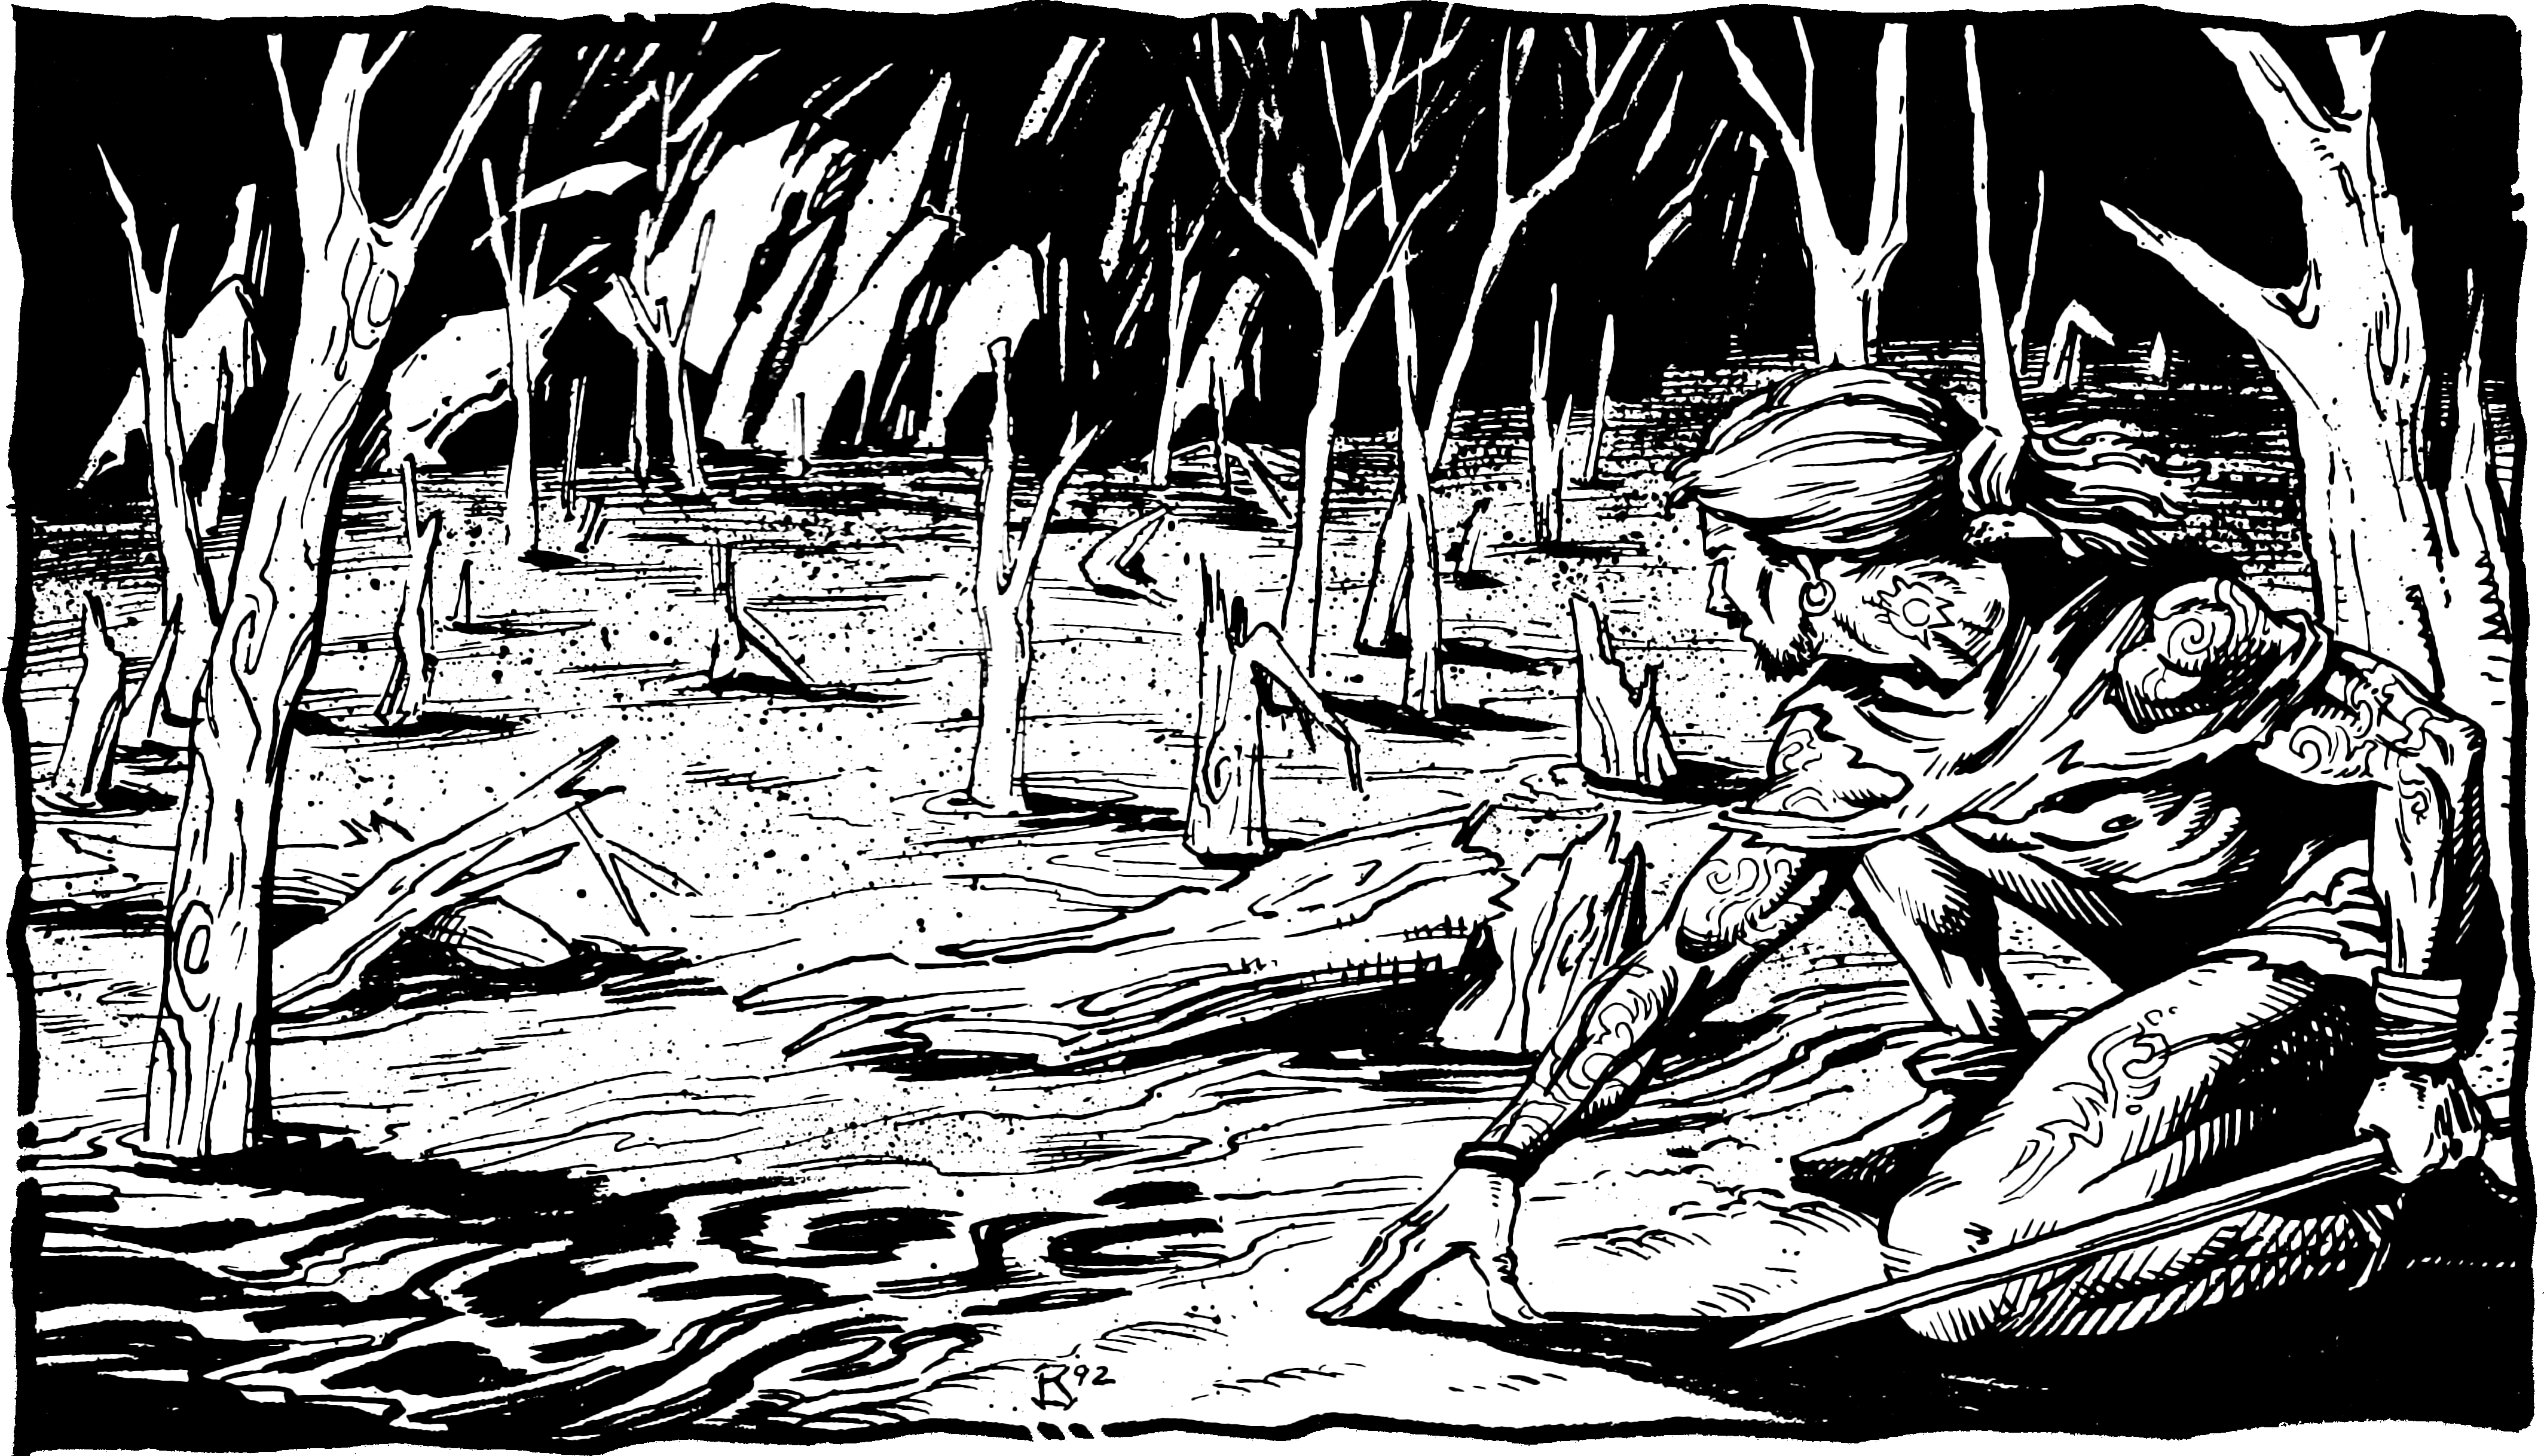
\includegraphics[width=\textwidth]{images/ranger-2.png}
\par\textit{\small\textcopyright Wizards of the Coast, 2020.}
\end{figure*}

\subsubsection{Class Features}
\textbf{Weapon and Armor Proficiency:} A ranger is proficient with all simple and martial weapons, and with light armor and shields (except tower shields).

\textbf{Favored Enemy (Ex):} At 1st level, a ranger may select a type of creature from among those given on \tabref{Athasian Favored Enemies}. The ranger gains a +2 bonus on \skill{Bluff}, \skill{Listen}, \skill{Sense Motive}, \skill{Spot}, and \skill{Survival} checks when using these skills against creatures of this type. Likewise, he gets a +2 bonus on weapon damage rolls against such creatures.

At 5th level and every five levels thereafter (10th, 15th, and 20th level), the ranger may select an additional favored enemy from those given on the table. In addition, at each such interval, the bonus against any one favored enemy (including the one just selected, if so desired) increases by 2.

If the ranger chooses humanoids or outsiders as a favored enemy, he must also choose an associated subtype, as indicated on the table. If a specific creature falls into more than one category of favored enemy, the ranger's bonuses do not stack; he simply uses whichever bonus is higher.

\Table{Athasian Favored Enemies}{X X}{
\tableheader Type (Subtype) & \tableheader Example\\
Aberration & gaj \\
Animal & lion \\
Construct & golem \\
Elemental (air) & air elemental beast \\
Elemental (earth) & crystal spider \\
Elemental (fire) & fire incarnation \\
Elemental (water) & rain paraelemental beast \\
Giant & beasthead giant \\
Humanoid (dwarf) & dwarf \\
Humanoid (elf) & elf \\
Humanoid (gith) & gith \\
Humanoid (halfling) & halfling \\
Humanoid (human) & human \\
Humanoid (jozhal) & jozhal \\
Humanoid (nikaal) & nikaal \\
Humanoid (psionic) & villichi \\
Humanoid (pterran) & pterran \\
Humanoid (reptilian) & silt runner \\
Humanoid (tarek) & tarek \\
Humanoid (tari) & tari \\
Magical beast & kirre \\
Monstrous humanoid & Thri-kreen \\
Outsider & silt half-elemental \\
Plant & hunting cactus \\
Undead & kaisharga \\
Vermin & kank}

\Table{Athasian Terrains}{X X}{
\tableheader Terrain Type & \tableheader Terrain Type\\
Boulder Field & Rocky Badland \\
Forest & Salt Flat \\
Jagged Cliffs & Sandy Waste \\
Mountain & Sea of Silt \\
Mud Flat & Stony Barren \\
Obsidian Waste & Swamp \\
Ocean & Verdant Belt}

\textbf{Favored Terrain (Ex):} At any time when a ranger could normally select a favored enemy, he may instead choose to select a favored terrain given on \tabref{Athasian Terrains}. A ranger receives a +2 bonus on \skill{Hide}, \skill{Listen}, \skill{Move Silently}, \skill{Search}, \skill{Spot} and \skill{Survival} checks made within your favored terrain. Likewise, he gets +2 bonus on \skill{Knowledge} (geography) and \skill{Knowledge} (nature) checks about your favored terrain.

This ability uses the same graduated progression that the favored enemy ability receives.

For example, at first level Sudatu selects monstrous humanoids as a favored enemy, receiving a +2 bonus when combating them. At fifth level, instead of taking a new favored enemy, he selects a Rocky Badlands as his favored terrain, and chooses to increase his favored enemy bonus to +4. At 10th level, Sudatu may again choose a new Favored Enemy, and may also choose between raising his favored enemy or favored terrain bonus by +2.

\textbf{Track:} A ranger gains \feat{Track} as a bonus feat.

\textbf{Wild Empathy (Ex):} A ranger can improve the attitude of an animal. This ability functions just like a \skill{Diplomacy} check to improve the attitude of a person. The ranger rolls 1d20 and adds his ranger level and his Charisma modifier to determine the wild empathy check result. The typical domestic animal has a starting attitude of indifferent, while wild animals are usually unfriendly.

To use wild empathy, the ranger and the animal must be able to study each other, which means that they must be within 9 meters of one another under normal visibility conditions. Generally, influencing an animal in this way takes 1 minute, but, as with influencing people, it might take more or less time.

The ranger can also use this ability to influence a magical beast with an Intelligence score of 1 or 2, but he takes a $-4$ penalty on the check.

\textbf{Combat Style (Ex):} At 2nd level, a ranger must select one of two combat styles to pursue: archery or two-weapon combat. This choice affects the character's class features but does not restrict his selection of feats or special abilities in any way.

If the ranger selects archery, he is treated as having the \feat{Rapid Shot} feat, even if he does not have the normal prerequisites for that feat.

If the ranger selects two-weapon combat, he is treated as having the \feat{Two-Weapon Fighting} feat, even if he does not have the normal prerequisites for that feat.

The benefits of the ranger's chosen style apply only when he wears light or no armor. He loses all benefits of his combat style when wearing medium or heavy armor.

\textbf{Endurance:} A ranger gains \feat{Endurance} as a bonus feat at 3rd level.

\textbf{Animal Companion (Ex):} At 4th level, a ranger gains an animal companion selected from the following list: badger, camel, dire rat, dog, riding dog, eagle, hawk, horse (light or heavy), owl, pony, snake (Small or Medium viper), or wolf. If the campaign takes place wholly or partly in an aquatic environment, the following creatures may be added to the ranger's list of options: manta ray, porpoise, Medium shark, and squid. This animal is a loyal companion that accompanies the ranger on his adventures as appropriate for its kind.

This ability functions like the druid ability of the same name, except that the ranger's effective druid level is one-half his ranger level. A ranger may select from the alternative lists of animal companions just as a druid can, though again his effective druid level is half his ranger level. Like a druid, a ranger cannot select an alternative animal if the choice would reduce his effective druid level below 1st.

\textbf{Spells:} Beginning at 4th level, a ranger gains the ability to cast a small number of divine spells, which are drawn from the ranger spell list. A ranger must choose and prepare his spells in advance (see below).

To prepare or cast a spell, a ranger must have a Wisdom score equal to at least 10 + the spell level. The Difficulty Class for a saving throw against a ranger's spell is 10 + the spell level + the ranger's Wisdom modifier.

Like other spellcasters, a ranger can cast only a certain number of spells of each spell level per day. His base daily spell allotment is given on \tabref{The Ranger}. In addition, he receives bonus spells per day if he has a high Wisdom score. When \tabref{The Ranger} indicates that the ranger gets 0 spells per day of a given spell level, he gains only the bonus spells he would be entitled to based on his Wisdom score for that spell level. The ranger does not have access to any domain spells or granted powers, as a cleric does.

A ranger prepares and casts spells the way a cleric does, though he cannot lose a prepared spell to cast a cure spell in its place. A ranger may prepare and cast any spell on the ranger spell list, provided that he can cast spells of that level, but he must choose which spells to prepare during his daily meditation.

Through 3rd level, a ranger has no caster level. At 4th level and higher, his caster level is one-half his ranger level.

\textbf{Improved Combat Style (Ex):} At 6th level, a ranger's aptitude in his chosen combat style (archery or two-weapon combat) improves. If he selected archery at 2nd level, he is treated as having the \feat{Manyshot} feat, even if he does not have the normal prerequisites for that feat.

If the ranger selected two-weapon combat at 2nd level, he is treated as having the \feat{Improved Two-Weapon Fighting} feat, even if he does not have the normal prerequisites for that feat.

As before, the benefits of the ranger's chosen style apply only when he wears light or no armor. He loses all benefits of his combat style when wearing medium or heavy armor.

\textbf{Woodland Stride (Ex):} Starting at 7th level, a ranger may move through any sort of undergrowth (such as natural thorns, briars, overgrown areas, and similar terrain) at his normal speed and without taking damage or suffering any other impairment.

However, thorns, briars, and overgrown areas that are enchanted or magically manipulated to impede motion still affect him.

\textbf{Swift Tracker (Ex):} Beginning at 8th level, a ranger can move at his normal speed while following tracks without taking the normal $-5$ penalty. He takes only a $-10$ penalty (instead of the normal $-20$) when moving at up to twice normal speed while tracking.

\textbf{Evasion (Ex):} At 9th level, a ranger can avoid even magical and unusual attacks with great agility. If he makes a successful Reflex saving throw against an attack that normally deals half damage on a successful save, he instead takes no damage. Evasion can be used only if the ranger is wearing light armor or no armor. A helpless ranger does not gain the benefit of evasion.

\textbf{Combat Style Mastery (Ex):} At 11th level, a ranger's aptitude in his chosen combat style (archery or two-weapon combat) improves again. If he selected archery at 2nd level, he is treated as having the \feat{Improved Precise Shot} feat, even if he does not have the normal prerequisites for that feat.

If the ranger selected two-weapon combat at 2nd level, he is treated as having the \feat{Greater Two-Weapon Fighting} feat, even if he does not have the normal prerequisites for that feat.

As before, the benefits of the ranger's chosen style apply only when he wears light or no armor. He loses all benefits of his combat style when wearing medium or heavy armor.

\textbf{Camouflage (Ex):} A ranger of 13th level or higher can use the \skill{Hide} skill in any sort of natural terrain, even if the terrain doesn't grant cover or concealment.

\textbf{Hide in Plain Sight (Ex):} While in any sort of natural terrain, a ranger of 17th level or higher can use the \skill{Hide} skill even while being observed.

\subsection{Playing a Ranger}

As a ranger, you nurture a close, almost mystical connection to the deadly terrain of Athas. To you, the burnt landscape is not a friend, but a well-respected adversary. Danger is always present, yet you understand it and even find a certain succor in living alongside it.

\subsubsection{Religion}

Many rangers pay homage to the elements, but a greater number honor the moons and the stars that guide them in the night---even though these celestial bodies do not have priests. In several city-states, particularly Gulg,
Kurn, and Eldaarich, many rangers owe fealty to the sorcerer-kings---virtually the entire noble caste of Gulg is comprised of rangers called judaga. Some rangers pay patronage to the Spirits of the Land, although these spirits do not bestow spells on rangers except those that multi-class as druid.

\subsubsection{Other Classes}

Rangers are slow to make friends with anyone, but have a particular affinity to druids, and to a lesser extent, barbarians and psions. Rangers tend not to lean on others for support and friendship, and often find it difficult to tolerate others who are quite different from themselves, such as talkative traders or controlling templars. Good rangers might simply try to avoid sharing a watch with a character that annoys them; neutral rangers tend to abandon annoying companions or just let them die; while evil rangers act friendly to the annoying companion and then slit their throat in their sleep.

Good rangers tend to hate defilers, although many rangers are ignorant of the distinction between preserving and defiling and hate wizards of all stripes. Strangely, many rangers have little objection to taking a companion who is of a favored enemy race, so long as that they are convinced that the companion is trustworthy and loyal.

\subsubsection{Combat}

Although you are a formidable warrior, you usually prefer not to stand against the sheer might of Athas' fighter, barbarians and gladiators. Your greatest ally is the environment itself. While in you favored terrain, you have a clear advantage over your adversaries. Try choosing favored enemies that are more common in your favored terrain.

As you advance, you are well served to invest in spells that have an effect other than dealing damage. If you can't drop a foe in one or two attacks, you can use entangle, snare, sting of the gold scorpion, or the like to make your opponents less dangerous in a prolonged fight.

\subsubsection{Advancement}

Perhaps the most dangerous place in Athas is inside a city-state: an environment rife with political intrigue, diseases, and assassination. To escape these noxious environs, you sought refuge in the wild where even the foulest elements of a society fear to tread. By gaining an intimate knowledge of this hazardous realm, you buy some breathing room and security from the urban madness.

As your ranger abilities increase, you find the Athasian wilderness a more and more inviting place (if a place with such constant peril can be called inviting). You can use your skills to establish safe havens for yourself or to gain employment opportunities---perhaps guiding a group of recently caught slaves through the Tyr valley or some noble into distant dangerous, location. You can also find that continuing to advance as a ranger or barbarian augments your already impressive abilities in the Athasian lands.

Continue to focus on skills such as Hive, Move Silently, and Survival. Spend discovered treasure on poison, magic weapons, and protective magic. The Mobility feat is good to consider, as is Nature's Child or Wastelander.

\subsection{Starting Packages}
\subsubsection{The Archer}
Elf Ranger

\textbf{Ability Scores:} Str 14, Dex 17, Con 10, Int 10, Wis 13, Cha 8.

\textbf{Skills:} \skill{Hide}, \skill{Listen}, \skill{Move Silently}, \skill{Spot}, \skill{Survival}.

\textbf{Languages:} Common, Elven.

\textbf{Feat:} \feat{Point Blank Shot}, \feat{Track}.

\textbf{Weapons:} Macahuitl (1d8/19--20)

Longbow with 20 arrows (1d8/$\times$3, 30 m).

\textbf{Armor:} Studded leather (+3 AC).

\textbf{Other Gear:} Standard adventurer's kit, 19 cp.

\subsubsection{The Scout}
Halfling Ranger

\textbf{Ability Scores:} Str 11, Dex 17, Con 12, Int 10, Wis 14, Cha 8.

\textbf{Skills:} \skill{Hide}, \skill{Knowledge} (nature), \skill{Listen}, \skill{Move Silently}, \skill{Spot}, \skill{Survival}.

\textbf{Languages:} Halfling.

\textbf{Feat:} \feat{Stealthy}, \feat{Track}.

\textbf{Weapons:} Macahuitl (1d6/19--20)

Small macahuitl (1d3/19--20)

Five javelins (1d4, 9 m).

\textbf{Armor:} Studded leather (+3 AC).

\textbf{Other Gear:} Standard adventurer's kit, 65 cp.

\subsubsection{The Wastelander}
Thri-kreen Ranger

\textbf{Ability Scores:} Str 14, Dex 19, Con 14, Int 8, Wis 15, Cha 4.

\textbf{Skills:} \skill{Hide}, \skill{Knowledge} (nature), \skill{Listen}, \skill{Move Silently}, \skill{Spot}, \skill{Survival}.

\textbf{Languages:} Kreen.

\textbf{Feat:} \feat{Track}, \feat{Wastelander}.

\textbf{Weapons:} Gythka (1d8/1d8)

Three chatkchas (1d6, 6 m).

\textbf{Armor:} Studded leather (+3 AC).

\textbf{Other Gear:} Standard adventurer's kit, 5 cp.

\subsection{Rangers on Athas}
\Quote{Trust me. He might not talk a lot and smell funnier than the rest of your men, but there is no other one I would bring along with me around the Great Ivory Plains.}{Waltian Inika, Gulg dune trader}

The Athasian wilderness is harsh and unforgiving, calling for skilled and capable men to master its ways---the ranger answers that challenge, living a rugged life through clever mastery of his surroundings. The ranger has a potent combination of stealth, woodcraft, magic, and fighting skill, making him the master of the wilderness.

\subsubsection{Daily Life}

A ranger adventures to learn about Athas, to protect nature, and to prove his superior hunting skills. Rangers spend their days in contemplation of nature, and tending their animal companions.

The Athasian ranger is a wanderer who hunts down a defiler to avenge himself for having his village destroyed, or a mercenary hunter for both monsters and humanoid creatures, or even a loner who simply prefers the company of animals.

\subsubsection{Notables}

Tales of halfling snipers are among the common Athasian legends. Any traveler to the Forest Ridge should rightfully fear the cannibals that move without a sound and strike without being seen. Thri-kreen are fabled for their rangers, as they are fast-moving relentless natural hunters, and their unarmed combat abilities become even more deadly when applied to subduing a quarry.

\subsubsection{Organizations}

There is no organized ranger organization; you are most likely to be a loner---or at best the leader of a group of raiders or renegades---than you are to gather with other rangers.

Often merchant houses are eager to employ you as a caravan guide through the most dangerous trade routes, or a city-state's templarate might hire you to provide a safe path to a templar patrol.

\subsubsection{NPC Reactions}

Within a city-state or large settlement, you find that you are either ignored or regarded with some small amount of curiosity. It is only after a city-dweller find himself outside the boundaries of his city-state that he truly appreciates you. Indeed, he holds you in the highest of regards, knowing that you are all that stands between him and a horrible death in the wastes.

\subsubsection{Ranger Lore}

Characters with ranks in \skill{Knowledge} (nature) can research rangers to learn more about them. When a character makes a skill check, read or paraphrase the following, including the information from lower DCs.

\textbf{DC 10:} Only those assisted by a ranger can hope to survive in the Athasian wilderness for long.

\textbf{DC 15:} Rangers move with ease through the harsh terrains that others find dangerous or impassable. They make of this aptitude to specialize in battling specific creatures of the wild.

\textbf{DC 20:} As a ranger advances in knowledge and skill, he grows more and more connected to the land, and eventually manages to draw spells from it.

\Class{Scout}
{Raiding tribe. Twenty footmen, three on kanks. They seem to be from the Mekillot Mountains. Be careful with the one wearing a kank's head.}
{Lobuu Airhunter, elf scout}

Scouts are invaluable assets for venturing the wastes, as any caravan master can tell. They can provide information about the surrounding area in time for any incoming battle. Scouts accomplish this by traveling faster than normal across difficult terrain, and specializing in keeping themselves unseen while detecting the foes and dangers ahead.

Merchant Houses are the primary employers for scouts around Athas, as they need to secure each caravan against not only the dangers of the wasteland but against ambushes from enemy houses. Each city-state also have some kind of division for scouts. Wars are a always about intelligence and logistics, and templars do not wish to fall in disgrace because of some blunder that could be avoided by deploying scouts. Scouts are also the primary military force on nomad tribes, since they need haste to move to new fields.

\WarriorTable{The Scout}{
1st  & +0         & +0 & +2  & +0 & Fast movement, skirmish (+1d6), trapfinding \\
2nd  & +1         & +0 & +3  & +0 & Uncanny dodge                               \\
3rd  & +2         & +1 & +3  & +1 & Skirmish (+1d6/+1 AC), trackless step       \\
4th  & +3         & +1 & +4  & +1 & Evasion                                     \\
5th  & +3         & +1 & +4  & +1 & Skirmish (+2d6/+1 AC)                       \\
6th  & +4         & +2 & +5  & +2 & Trade secret                                \\
7th  & +5         & +2 & +5  & +2 & Skirmish (+2d6/+2 AC)                       \\
8th  & +6/+1      & +2 & +6  & +2 & Bonus feat, camouflage                      \\
9th  & +6/+1      & +3 & +6  & +3 & Skirmish (+3d6/+2 AC)                       \\
10th & +7/+2      & +3 & +7  & +3 & Special ability, trade secret               \\
11th & +8/+3      & +3 & +7  & +3 & Skirmish (+3d6/+3 AC)                       \\
12th & +9/+4      & +4 & +8  & +4 & Bonus feat                                  \\
13th & +9/+4      & +4 & +8  & +4 & Skirmish (+4d6/+3 AC)                       \\
14th & +10/+5     & +4 & +9  & +4 & Hide in plain sight, trade secret           \\
15th & +11/+6/+1  & +5 & +9  & +5 & Special ability, skirmish (+4d6/+4 AC)      \\
16th & +12/+7/+2  & +5 & +10 & +5 & Bonus feat                                  \\
17th & +12/+7/+2  & +5 & +10 & +5 & Skirmish (+5d6/+4 AC)                       \\
18th & +13/+8/+3  & +6 & +11 & +6 & Free movement, trade secret                 \\
19th & +14/+9/+4  & +6 & +11 & +6 & Skirmish (+5d6/+5 AC)                       \\
20th & +15/+10/+5 & +6 & +12 & +6 & Bonus feat, special ability                 \\
}

\subsection{Making a Scout}
Since scouts are more fragile and have less combat effectiveness than a mul fighter or a half-giant barbarian, they are not meant to fight fairly. Scouts focus on always being at an advantage: they are always on the move, stay hidden whenever possible, and use difficult terrain as safety against their enemies. Most of their class features aren't unique to them, but their combination makes scout the best survivalist.

\textbf{Races:} Elves make the majority of Athasian scouts, due to their faster movement and their nomad culture that relies on scouts to warn the tribe of any dangers further ahead. Human and half-elf scouts are usually hired by merchant houses to attend to caravans and prevent them to stumble upon any monsters or ambushes. Halflings also employ scouts in the Forest Ridge, as a way to prepare ambushes against any big-folk trying to invade their land. Thri-kreen use scouts in their all their packs: hunting packs need scouts to search for fresh quarry, while raiding packs look for vulnerable (and tasty) prey. Dwarves, muls, and half-giants don't usually are scouts as their races are too bulky to be successful scouts.

\textbf{Alignment:} Scouts can fit into any society, and can be of any alignment. Those in a military organization are usually lawful, while those in nomad tribes are usually chaotic. But scouts have no restriction whatsoever.

\Figure[\columnwidth+2mm]{t}{images/adventurer-4.png}
\subsection{Game Rule Information}
\textbf{Hit Die:} d8.

\subsubsection{Class Skills}
\skill{Balance} (Dex),
\skill{Climb} (Str),
\skill{Craft} (Int),
\skill{Escape Artist} (Dex),
\skill{Hide} (Dex),
\skill{Jump} (Str),
\skill{Knowledge} (dungeoneering) (Int),
\skill{Knowledge} (geography) (Int),
\skill{Knowledge} (nature) (Int),
\skill{Knowledge} (warcraft) (Int),
\skill{Listen} (Wis),
\skill{Move Silently} (Dex),
\skill{Ride} (Wis),
\skill{Search} (Int),
\skill{Sense Motive} (Wis),
\skill{Speak Language} (N/A),
\skill{Spot} (Wis),
\skill{Survival} (Wis),
\skill{Tumble} (Dex),
and \skill{Use Rope} (Dex).

\textbf{Skill Points per Level:} 8 + Int modifier ($\times4$ at 1st level).

\Figure{t}{images/ranger-1.png}
\subsubsection{Class Features}
\textbf{Weapon and Armor Proficiency:} Scouts are proficient with all simple weapons, plus the handaxe, short sword, and shortbow. Scouts are proficient with light armor, but not with shields.


\textbf{Fast Movement (Ex):} A scout's land speed is faster than the norm for his race by +3 meters. A scout loses this benefit when wearing medium or heavy armor or when carrying a medium or heavy load.


\textbf{Skirmish (Ex):} A scout relies on mobility to deal extra damage and improve his defense. He deals an extra 1d6 points of damage on all attacks he makes during any round in which he moves at least 3 meters. The extra damage applies only to attacks taken during the scout's turn. This extra damage increases by 1d6 for every four levels gained above 1st (2d6 at 5th, 3d6 at 9th, 4d6 at 13th, and 5d6 at 17th level).

The extra damage only applies against living creatures that have a discernible anatomy. Undead, constructs, oozes, plants, incorporeal creatures, and creatures immune to extra damage from critical hits are not vulnerable to this additional damage. The scout must be able to see the target well enough to pick out a vital spot and must be able to reach such a spot. Master scouts can apply this extra damage to ranged attacks made while skirmishing, but only if the target is within 9 meters.

At 3rd level, a scout gains a +1 competence bonus to Armor Class during any round in which he moves at least 3 meters. The bonus applies as soon as the scout has moved 3 meters, and lasts until the start of his next turn. This bonus improves by 1 for every four levels gained above 3rd (+2 at 7th, +3 at 11th, +4 at 15th, and +5 at 19th level).

A scout loses this ability when wearing medium or heavy armor or when carrying a medium or heavy load. If he gains the skirmish ability from another source, the bonuses stack.


\textbf{Trapfinding:} Scouts can use the \skill{Search} skill to locate traps when the task has a Difficulty Class higher than 20.

Finding a nonmagical trap has a DC of at least 20, or higher if it is well hidden. Finding a magic trap has a DC of 25 + the level of the spell used to create it.

Scouts can use the \skill{Disable Device} skill to disarm magic traps. A magic trap generally has a DC of 25 + the level of the spell used to create it.

A scout who beats a trap's DC by 10 or more with a \skill{Disable Device} check can study a trap, figure out how it works, and bypass it (with his party) without disarming it.


\textbf{Uncanny Dodge (Ex):} Starting at 2nd level, a scout can react to danger before his senses would normally allow him to do so. He retains his Dexterity bonus to AC (if any) even if he is caught flat-footed or struck by an invisible attacker. However, he still loses his Dexterity bonus to AC if immobilized.

If a scout already has uncanny dodge from a different class he automatically gains improved uncanny dodge instead.


\textbf{Trackless Step (Ex):} Starting at 3rd level, a scout leaves no trail in natural surroundings and cannot be tracked. He may choose to leave a trail if so desired.


\textbf{Evasion (Ex):} At 4th level and higher, a scout can avoid even magical and unusual attacks with great agility. If he makes a successful Reflex saving throw against an attack that normally deals half damage on a successful save, he instead takes no damage. Evasion can be used only if the scout is wearing light armor or no armor. A helpless scout does not gain the benefit of evasion.


\textbf{Trade Secrets:} At 6th level and every four levels thereafter (10th, 14th, and 18th level), a scout learns a trade secret chosen from the list below.

\textit{Accurate (Ex):} When a scout with this trade secret attacks, his accuracy allows him to ignore a number of points of armor or natural armor bonus to AC equal to \onequarter his scout level.

\textit{Battle Fortitude (Ex):} A scout adds \onequarter his scout level as a competence bonus on Fortitude saves and initiative checks. A scout loses this benefit when wearing medium or heavy armor or when carrying a medium or heavy load.

\textit{Deadly Range (Ex):} A scout with this talent increases the range at which he can deal skirmish damage by 6 meters. A scout can select this talent more than once; its effects stack.

\textit{Faster Movement (Ex):} A scout increases his land speed by +3 meters. This accumulates with the fast movement ability. A scout loses this benefit when wearing medium or heavy armor or when carrying a medium or heavy load.

\textit{Flawless Stride (Ex):} A scout can move through any sort of terrain that slows movement (such as undergrowth, rubble, and similar terrain) at his normal speed and without taking damage or suffering any other impairment.

This ability does not let him move more quickly through terrain that requires a \skill{Climb} or \skill{Swim} check to navigate, nor can he move more quickly through terrain or undergrowth that has been magically manipulated to impede motion.

A scout loses this benefit when wearing medium or heavy armor or when carrying a medium or heavy load.

\textit{Poison Use:} A scout never risk accidentally poisoning himself when applying poison to a blade.

\textit{Resilient (Ex):} A scout with this trade secret adds \onehalf his scout level as a luck bonus to saving throws against poisons, spells, and spell-like abilities.

\textit{Seasoned Explorer (Ex):} A scout of 14th level or higher can make \skill{Survival} checks while moving at his full overland speed without the $-30$ penalty.

\textit{Scout Feat:} A scout may select an ambush feat\textsuperscript{CS}, a skill feat, or \feat{Skill Focus} in place of a trade secret. He must meet all the prerequisites for the feat. This trade secret may be chosen more than once, each time the scout must select a different feat.

\textit{Skilled:} A scout with this trade secret adds \onequarter your scout level as a competence bonus to one of the following skills: \skill{Balance}, \skill{Climb}, \skill{Hide}, \skill{Listen}, \skill{Move Silently}, \skill{Ride}, \skill{Search}, \skill{Spot}, \skill{Survival}. This trade secret may be chosen more than once, each time it applies to a different skill.

\textit{Versatile:} A scout with this trade secret selects any two non-class skills to be considered class skills.


\textbf{Bonus Feat:} At 8th level and every four levels thereafter (12th, 16th, and 20th level), a scout gains a bonus feat, which must be selected from the following list:
\feat{Blind-Fight},
Bounding Assault\textsuperscript{PH2},
Brachiation\textsuperscript{CA},
\feat{Combat Expertise},
Danger Sense\textsuperscript{CA},
Dash\textsuperscript{CW},
\feat{Dodge},
\feat{Endurance},
\feat{Far Shot},
Hear the Unseen\textsuperscript{CA},
\feat{Improved Initiative},
Improved Skirmish\textsuperscript{CS},
Improved Swimming\textsuperscript{CA},
Keen-Eared Scout\textsuperscript{PH2},
Melee Evasion\textsuperscript{PH2},
\feat{Mobility},
\feat{Point Blank Shot},
\feat{Precise Shot},
\feat{Quick Draw},
Quick Reconnoiter\textsuperscript{CA},
\feat{Rapid Reload},
\feat{Shot On The Run},
\feat{Spring Attack},
\feat{Track},
\feat{Wastelander}.
He must meet all the prerequisites for the feat.


\textbf{Camouflage (Ex):} A scout of 8th level or higher can use the \skill{Hide} skill in any sort of natural terrain, even if the terrain doesn't grant cover or concealment.


\textbf{Special Ability:} On attaining 10th level, and at every five levels thereafter (15th, and 20th), a scout gains a special ability of his choice from among the following options.

\textit{Blindsense (Ex):} A scout gains the blindsense ability out to 9 meters. He does not need to make \skill{Spot} or \skill{Listen} checks to notice and locate creatures within range of his blindsense ability, provided that he has line of effect to that creature. Any opponent the scout cannot see has total concealment (50\% miss chance) against him, and the scout still has the normal miss chance when attacking foes that have concealment. Visibility still affects the scout's movement. A scout is still denied its Dexterity bonus to Armor Class against attacks from creatures he cannot see.

\textit{Defensive Roll (Ex):} A scout learns how to avoid a potentially lethal blow to take less damage from it than he otherwise would. Once per day, when he would be reduced to 0 or fewer hit points by damage in combat (from a weapon or other blow, not a spell or special ability), the scout can attempt to roll with the damage. To use this ability, the scout must attempt a Reflex saving throw (DC = damage dealt). If the save succeeds, he takes only half damage from the blow; if it fails, he takes full damage. He must be aware of the attack and able to react to it in order to execute his defensive roll---if he is denied his Dexterity bonus to AC, he can't use this ability. Since this effect would not normally allow a character to make a Reflex save for half damage, the rogue's evasion ability does not apply to the defensive roll.

\textit{Favored Terrain (Ex):} A scout chooses a terrain given on \tabref{Athasian Terrains} to specialize. He receives a +2 bonus on \skill{Hide}, \skill{Listen}, \skill{Move Silently}, \skill{Search}, \skill{Spot} and \skill{Survival} checks made within your favored terrain. Likewise, he gets +2 bonus on \skill{Knowledge} (geography) and \skill{Knowledge} (nature) checks about your favored terrain.

If a scout also has ranger levels, this ability uses the same graduated progression that the favored terrain ability receives.

\textit{Improved Evasion (Ex):} This ability works like evasion, except that while the scout still takes no damage on a successful Reflex saving throw against attacks henceforth she takes only half damage on a failed save. A helpless scout does not gain the benefit of improved evasion.

\textit{Trap Sense (Ex):} If a scout passes within 1.5 meter of a trap, she is entitled to a \skill{Search} check to notice it as if she was actively looking for it.

\textit{Feat:} A scout may gain a bonus feat in place of a special ability.


\textbf{Hide in Plain Sight (Ex):} While in any sort of natural terrain, a scout of 14th level or higher can use the \skill{Hide} skill even while being observed.


\textbf{Free Movement (Ex):} At 18th level and higher, a scout can slip out of bonds, grapples, and even the effects of confining spells easily. This ability duplicates the effect of a \spell{freedom of movement} spell, except that it is always active. A scout loses this benefit when wearing medium or heavy armor or when carrying a medium or heavy load.



\subsection{Playing a Scout}
Scouts trained in the military rarely have the time to go in adventures. An adventuring scout usually comes from nomad tribes or rural villages, or even ex-military who left the service behind. They respect the dangers ahead, as their function is primarily to detect dangers and not to face them.

\subsubsection{Religion}
Scouts are generally not devoted to any element. Scouts in service of any infantry might pay homage to the element their cleric is devoted, while those in nomad tribes pay homage to the Spirits of the Land.

\subsubsection{Other Classes}
Scouts don't have problems with any class, as long as they get to do their job unimpeded. When they need to run ahead, they will not slow down because of fighter on a heavy armor. Scouts have great affinity with barbarians and rangers. They can either keep up with scouts as they travel, or they can stay undetected while they make any observation.

\subsubsection{Combat}
You serve as a backup melee combatant or ranged expert in battle. Your role is to support any warrior in the group, with your unique combat style. Scouts shine best in large battlefields where you can be always on the move, and in difficult terrains where you can walk in greater rate than your enemies. As a scout, you are not expected to fight fair, so use the environment as best as you can to hit and not be hit.

\subsubsection{Advancement}
Depending on your role and what is expected in your adventures, taking assigning skill points to the available \skill{Knowledge} fields is essential to be able to understand what dangers actually lie ahead. Likewise, \skill{Hide}, \skill{Listen}, \skill{Move Silently}, and \skill{Spot} are a vital part of scouting since detecting trouble from further distances while being undetected improves your chances to survive another day. Melee scouts tend to depend on \skill{Tumble} to move within their enemies' reach.

Due to your combat style, it is natural to take either the \feat{Shot on the Run} feat or the \feat{Spring Attack} feat, and all their prerequisites. Taking Improved Skirmish\textsuperscript{CS} is also expected at higher levels. If you wander too much on the wilderness, consider becoming a \class{Master Scout}.

\subsection{Starting Packages}
\subsubsection{The Archer}
Elf Scout

\textbf{Ability Scores:} Str 14, Dex 17, Con 10, Int 10, Wis 13, Cha 8.

\textbf{Skills:} \skill{Balance}, \skill{Climb}, \skill{Hide}, \skill{Listen}, \skill{Move Silently}, \skill{Search}, \skill{Spot}, \skill{Survival}, \skill{Tumble}, \skill{Use Rope}.

\textbf{Languages:} Common, Elven.

\textbf{Feat:} \feat{Point Blank Shot}.

\textbf{Weapons:} Dagger (1d4/19--20)

Shortbow with 20 arrows (1d6/$\times$3, 30 m).

\textbf{Armor:} Studded leather (+3 AC).

\textbf{Other Gear:} Standard adventurer's kit, 19 cp.

\subsubsection{The Dervish}
Halfling Scout

\textbf{Ability Scores:} Str 11, Dex 17, Con 12, Int 10, Wis 14, Cha 8.

\textbf{Skills:} \skill{Balance}, \skill{Escape Artist}, \skill{Hide}, \skill{Jump}, \skill{Listen}, \skill{Move Silently}, \skill{Sense Motive}, \skill{Spot}, \skill{Survival}, \skill{Tumble}.

\textbf{Languages:} Halfling.

\textbf{Feat:} \feat{Dodge}.

\textbf{Weapons:} Dagger (1d3/19--20)

Small longspear (1d6/$\times$3)

Five javelins (1d4, 9 m).

\textbf{Armor:} Studded leather (+3 AC).

\textbf{Other Gear:} Standard adventurer's kit, 65 cp.

\subsubsection{The Pathfinder}
Thri-kreen Scout

\textbf{Ability Scores:} Str 14, Dex 19, Con 14, Int 8, Wis 15, Cha 4.

\textbf{Skills:} \skill{Climb}, \skill{Hide}, \skill{Knowledge} (nature), \skill{Knowledge} (warcraft), \skill{Listen}, \skill{Move Silently}, \skill{Search}, \skill{Spot}, \skill{Survival}.

\textbf{Languages:} Kreen.

\textbf{Feat:} \feat{Wastelander}.

\textbf{Weapons:} Gythka (1d8/1d8)

Three chatkchas (1d6, 6 m).

\textbf{Armor:} Studded leather (+3 AC).

\textbf{Other Gear:} Standard adventurer's kit, 5 cp.

\subsection{Scouts on Athas}
\Quote{I need you four to run ahead and tell me what you see ten kilometers in every direction. The winds have told me to be careful early this morning and we don't want to lose any more kanks to raiders. See that you come back in two hours: we need to move.}{Krensh, leader of a nomad tribe}

Scouts are part of any group that needs to move frequently: city-state armies, merchant houses, nomad tribes, even halflings in the Forest Ridge or the Kreen. They are the go-to for reconnaissance all over Athas.

\subsubsection{Daily Life}
Scouts are adventurers because of their trade: their job is to venture ahead of their group, to discover what is at the edge of the horizon and come back to tell their tale. They do this while being hunters, soldiers, or guides.

Their class doesn't define as much of their live as their employers. An army scout has a rigid routine, while a nomad hunter has to adapt to their new environment each day.

\subsubsection{Notables}
The Kreen Empire uses scouts to gather information on the Tablelands, in case any sorcerer-king make a move against the Empire. Some of those scouts stay in the city-states: those are the thor-kreen.

\subsubsection{Organizations}
Scouts are never in an organization of their own, but as part of many greater ones. Joining an organization is part of their trade, as this is the easiest way for most scouts to guarantee their livelihood. Only those who are alone in the wastes by choice have no need for a patron organization.

\subsubsection{NPC Reactions}
Scouts are of little interest for the common people, since they don't have a glorious job as gladiators, nor have any impressive feat to accomplish. But all bards know the value of the information scouts provide and are quite fond of drunk scouts in any tavern. Nomad tribesmen also appreciate information and services of scouts to protect their tribes.

\subsubsection{Scout Lore}
Characters with ranks in \skill{Knowledge} (warcraft) can research scouts to learn more about them. When a character makes a skill check, read or paraphrase the following, including the information from lower DCs.

\textbf{DC 10:} Scouts serve to alert you of dangers ahead. They can spot hidden traps.

\textbf{DC 15:} Scouts are fast and move with ease through the harsh terrains that others find dangerous or impassable.

\textbf{DC 20:} Highly skilled scouts leave no trail and can disappear from sight at a moment's notice.

\Class{Templar}
{Against the law? The law is a convenience, a tool for us to use as we will, not a yoke bound to our necks. Laws are guidelines, not rules cast in iron. Stretching them is not the same as breaking them, my young apprentice. Take that to heart, for if you accuse me again, I will have your heart served cold.}{Zelgado De'Draigee, human templar}

Templars are civil servants within a city-state's government organization commonly referred to as a ``temple,'' ``bureau,'' or ``order.'' Each templar swears obedience to his temple, and absolute fealty to his sorcerer-king. In return, the sorcerer-king grants them spell power stolen from the elemental planes.

In most city-states, templars are the ultimate authority---judge, jury, and executioner. Templars police and administer the city-states, and serve other civil roles ranging from general to jailor and from tax collector to garbage collector.

\SpellcasterTable{4mm}{The Templar}{
\SpellHeader{9} \\
1  & +0         & +2  & +0 & +2  & Assume domain, secular aptitude, sigil & 5 & 3+1 &&&&&&&&\\
2  & +1         & +3  & +0 & +3  &                                        & 6 & 4+1 &&&&&&&&\\
3  & +2         & +3  & +1 & +3  &                                        & 6 & 5+1 &&&&&&&&\\
4  & +3         & +4  & +1 & +4  & Turn or rebuke undead                  & 6 & 6+1 & 3+1 &&&&&&&\\
5  & +3         & +4  & +1 & +4  &                                        & 6 & 6+1 & 4+1 &&&&&&&\\
6  & +4         & +5  & +2 & +5  & \feat{Scribe Scroll}                   & 6 & 6+1 & 5+1 & 3+1 &&&&&&\\
7  & +5         & +5  & +2 & +5  &                                        & 6 & 6+1 & 6+1 & 4+1 &&&&&&\\
8  & +6/+1      & +6  & +2 & +6  & \feat{Brew Potion}                     & 6 & 6+1 & 6+1 & 5+1 & 3+1 &&&&&\\
9  & +6/+1      & +6  & +3 & +6  &                                        & 6 & 6+1 & 6+1 & 6+1 & 4+1 &&&&&\\
10 & +7/+2      & +7  & +3 & +7  &                                        & 6 & 6+1 & 6+1 & 6+1 & 5+1 & 3+1 &&&&\\
11 & +8/+3      & +7  & +3 & +7  &                                        & 6 & 6+1 & 6+1 & 6+1 & 6+1 & 4+1 &&&&\\
12 & +9/+4      & +8  & +4 & +8  &                                        & 6 & 6+1 & 6+1 & 6+1 & 6+1 & 5+1 & 3+1 &&&\\
13 & +9/+4      & +8  & +4 & +8  &                                        & 6 & 6+1 & 6+1 & 6+1 & 6+1 & 6+1 & 4+1 &&&\\
14 & +10/+5     & +9  & +4 & +9  &                                        & 6 & 6+1 & 6+1 & 6+1 & 6+1 & 6+1 & 5+1 & 3+1 &&\\
15 & +11/+6/+1  & +9  & +5 & +9  &                                        & 6 & 6+1 & 6+1 & 6+1 & 6+1 & 6+1 & 6+1 & 4+1 &&\\
16 & +12/+7/+2  & +10 & +5 & +10 &                                        & 6 & 6+1 & 6+1 & 6+1 & 6+1 & 6+1 & 6+1 & 5+1 & 3+1 &\\
17 & +12/+7/+2  & +10 & +5 & +10 &                                        & 6 & 6+1 & 6+1 & 6+1 & 6+1 & 6+1 & 6+1 & 6+1 & 4+1 &\\
18 & +13/+8/+3  & +11 & +6 & +11 &                                        & 6 & 6+1 & 6+1 & 6+1 & 6+1 & 6+1 & 6+1 & 6+1 & 5+1 & 3+1 \\
19 & +14/+9/+4  & +11 & +6 & +11 &                                        & 6 & 6+1 & 6+1 & 6+1 & 6+1 & 6+1 & 6+1 & 6+1 & 6+1 & 4+1 \\
20 & +15/+10/+5 & +12 & +6 & +12 &                                        & 6 & 6+1 & 6+1 & 6+1 & 6+1 & 6+1 & 6+1 & 6+1 & 6+1 & 5+1
}
\begin{figure}[t!]
\centering
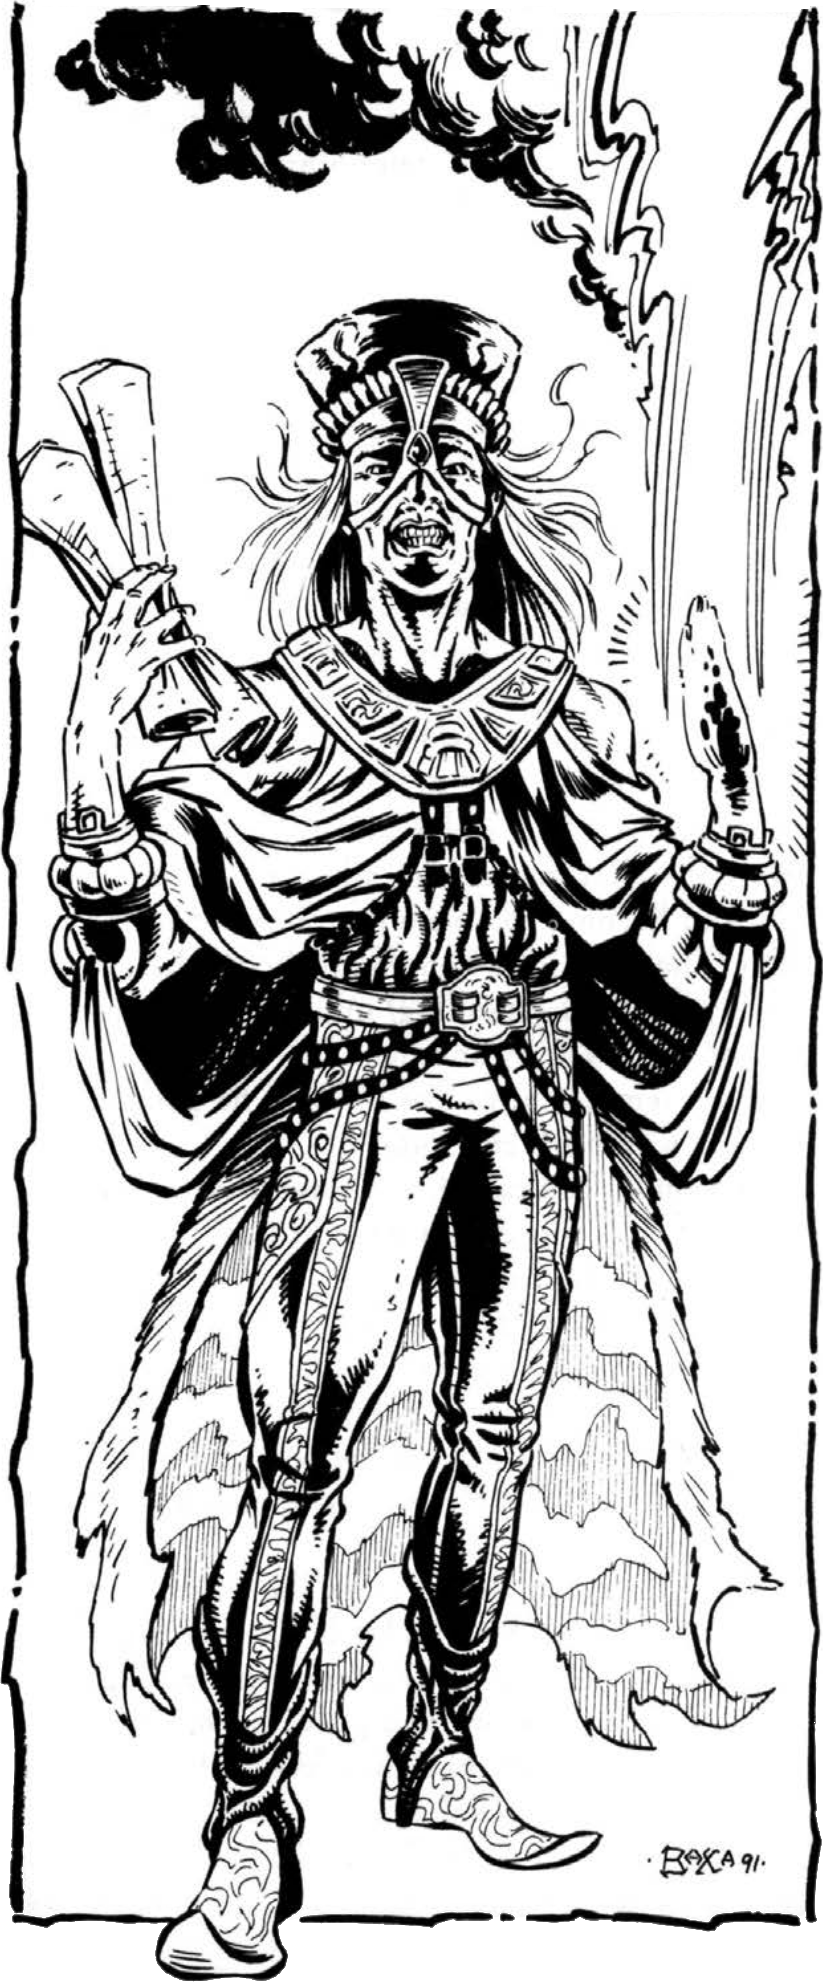
\includegraphics[width=\columnwidth]{images/templar-1.png}
\WOTC
\end{figure}

\subsection{Making a Templar}
Templars can cast a number of divine spells each day, as granted by their lord. If necessary they can be a destructive fighting force, but they serve much better as officers of slave-soldiers, mercenaries, or undead. Their wide array of available skills reflects the equally wide array of roles that Templars fill as servants of the sorcerer-kings and queens.

\textbf{Abilities:} If you want to make good use of your templar spells and you secular aptitude, you'll need a high Charisma. As with any melee-oriented class, Strength is a key ability for templars and Constitution provides you with increased ht points as usual.

\textbf{Races:} While the need for religion and divine magic is nearly universal on Athas, the need for specialized militant priest--bureaucrats is peculiar to large city-states dominated by sorcerer-kings. While in theory, no sentient race is precluded from the templar class, in practice, a sorcerer-king grant spells only to those who he wants to represent him. Humans dominate the templar priesthoods of all city-states except for New Giustenal. Dwarves, muls, and half-elves commonly become templars in many cities, while elves are less commonly accepted. Templars of other races are rare or unheard--of in most cities.

\textbf{Alignment:} A templar's alignment must be within one step of his sorcerer-king's (that is, it may be one step away on either the lawful--chaotic axis or the good--evil axis, but not both). Because of that, templars are almost never good. The laws they uphold are corrupt; the monarchs they serve are arguably the vilest creatures on the face of Athas, and often the templars are cruel and unjust themselves. However, many templars take considerable pride in the prosperity and magnificence of their city-state, and in the well--oiled machine of their order. Templars are most commonly lawful neutral or lawful evil.

\subsection{Game Rule Information}

\textbf{Alignment:} A templar's alignment must be within one step of his sorcerer-monarch's in each axis (that is, it may be one step away on the lawful-chaotic axis or the good-evil axis, but not two steps in either of them). A cleric may not be neutral unless his sorcerer-monarch's alignment is also neutral.

\textbf{Hit Die:} d8.

\subsubsection{Class Skills}
\skill{Appraise} (Int), \skill{Bluff} (Cha), \skill{Concentration} (Con), \skill{Craft} (Int), \skill{Diplomacy} (Cha), \skill{Forgery} (Int), \skill{Gather Information} (Cha), \skill{Heal} (Wis), \skill{Intimidate} (Cha), \skill{Knowledge} (all skills individually) (Int), \skill{Literacy} (N/A), \skill{Profession} (Wis), \skill{Sense Motive} (Wis), \skill{Spellcraft} (Int), and \skill{Spot} (Wis).

\textbf{Skill Points per Level:} 4 + Int modifier ($\times 4$ at 1st level).

\subsubsection{Class Features}

\textbf{Weapon and Armor Proficiency:} Templars are proficient in all simple weapons. Since templar training involves some education in warfare, templars receive two martial weapons proficiencies. Templars are proficient in light and medium armor and shields (except tower shields).

\textbf{Spellcasting:} A templar casts divine spells, which are drawn from the templar spell list. When she gain access to a new level of spells, she automatically knows all the spells for that level on the templar's spell list. She can cast any spell she know without preparing it ahead of time. Essentially, her spell list is the same as her spells known list.

To cast a spell, a templar must have a Charisma score of 10 + the spell's level. The Difficulty Class for a saving throw against a templar's spell is 10 + the spell's level + the templar's Cha modifier. Like other spellcasters, a templar can cast only a certain number of spells of each level per day. The base daily allotment is given on \tabref{The Templar}. In addition, she receives bonus spells if she has a high Charisma score.

She can also cast one domain spell of each spell level per day, as a cleric does. The domain spell is chosen at the time of casting from the spells associated with your assumed domains (see below), as she casts spells spontaneously and need not prepare spells ahead of time.

A templar need not prepare spells in advance. She can cast any spell she knows at any time, assuming she has not yet used up your spells per day for that spell level.

Templars use their sorcerer-king's sigil as divine focus.

\textbf{Assume Domain:} A templar is assigned two domains based on her sorcerer-monarch. Each domain gives her access to a domain spell at each spell level she can cast, from 1st on up, as well as a granted power. She gets the granted powers of both the assumed domains. With access to two domain spells at a given spell level, she adds only one of those spells to your spells known list.

\Table{Sorcerer-Kings' Domains and Alignment}{l X l}{
\tableheader Sorcerer-Monarch & \tableheader Domains & \tableheader Alignment\\
Abalach-Re & Chaos, Charm & Chaotic Evil \\
Andropinis & Law, Nobility & Neutral Evil \\
Borys & Destruction, Protection & Lawful Evil \\
Daskinor & Chaos, Madness & Lawful Evil \\
Dregoth & Death, Destruction & Chaotic Evil \\
Hamanu & Strength, War$\dagger$ & Neutral Evil \\
Kalak & Magic, Trickery & Neutral Evil \\
Lalali-Puy & Animal, Plant & Neutral Evil \\
Nibenay & Magic, Mind & Neutral Evil \\
Oronis & Knowledge, Protection & Neutral Good \\
Tectuktitlay & Glory, Strength & Neutral Evil \\
\rowcolor{white}
\multicolumn{3}{l}{$\dagger$ Hamanu's favored weapon is the longsword.}
}

\textbf{Secular Aptitude (Ex):} A templar gains \feat{Secular Authority} as a bonus feat. In addition, she receives a competence bonus to Secular Authority checks equal to half her class level.

\textit{Sigil} \textbf{(Sp):} Every templar receives a sigil that is the sign of their rank and station as a templar within their city's templarate. The form of the sigil is unique to each city-state, but is always unmistakable for what it is. The sigil serves as your divine focus, and also allows you to use the spell-like powers \spell{arcane mark}, \spell{purify food and drink}, and \spell{slave scent} a combined total of times equal to 3 + your Cha modifier. These spell-like powers do not count against your total of spells per day.

\textbf{Turn or Rebuke Undead (Su):} Any templar, regardless of alignment, has the power to affect undead creatures by channeling the power of his sorcerer-king through his sigil.

A good templar (or a neutral templar who worships a good sorcerer-king) can turn or destroy undead creatures. An evil templar (or a neutral templar who worships an evil sorcerer-king) instead rebukes or commands such creatures. A neutral templar of a neutral sorcerer-king must choose whether his turning ability functions as that of a good templar or an evil templar. Once this choice is made, it cannot be reversed.

A templar may attempt to turn undead a number of times per day equal to 3 + your Charisma modifier. A templar with 5 or more ranks in \skill{Knowledge} (religion) gets a +2 bonus on turning checks against undead. A templar turns undead as a cleric of three levels lower would.

\textbf{Scribe Scroll:} At 6th level, a templar gains \feat{Scribe Scroll} as a bonus feat.

\textbf{Brew Potion:} At 8th level, a templar gains \feat{Brew Potion} as a bonus feat.

\subsubsection{Ex-Templars}
A templar who displeases or abandons his sorcerer-monarch, or one whose sorcerer-monarch dies, loses all templar spellcasting abilities. An ex-templar is treated as a member of an NPC class (commoner, expert, etc) for purposes of determining CR. If the templar later becomes the templar of another sorcerer-monarch, he immediately regains his full templar spellcasting abilities.

\subsection{Playing a Templar}

A templar can take the fighter's place in the front ranks of a party or ensorcel his foes from a distance like a cleric. While you aren't quite as good as either a dedicated fighter or a dedicated cleric or psion in those roles, you're reasonably effective in either, and you can change roles on a round-by-round basis as needed.

As a templar, you believe the acquisition of power and influence is a worthy end in itself. By having power, you can effect your will in the world, be it good or bad. Those who have or seek power deserve your respect, while those who have power but fail to use it deserve your derision.

You adventure out of a desire to gain more power and influence in every quest. Drawn by your power, others follow your lead, and you are happy to command them.

\subsubsection{Religion}
The reverence of templars and their respective sorcerer-monarch varies greatly with the city-state. Some rulers, like Hamanu or Lalali-Puy, claim they are gods and demand their citizen and templars to worship them as such. Other, like Nibenay and Andropinis, only require service, not worship, from their templars.

\subsubsection{Other Classes}
Templars sometimes clash with druids and elemental clerics, who represent an older, more primal relationship between mortal, nature, and the elements. Templars tend to tolerate these ``primitive priests,'' as long as the druids and clerics do not share their opinions that sorcerer-kings are usurpers of profane divine elemental power. Templars get along with most other classes very well, provided of course that a templar is in charge.

\subsubsection{Combat}
Most of a templar's spells target a single target or have a range of touch, so you are most effective when you single out and focus upon defeating a single opponent. Your spells that affect areas are limited mostly to cones,
which means you need to be on or near the front lines to get the greatest effect from them. Even if you come close to being effective as a fighter or cleric in his chosen field, you're certainly not as effective as a fighter and a cleric.

Outside combat, use your secular authority to its greatest advantage, securing troops and resources for when it happens. If you have a cleric or other healer in the group, save your cures for emergency healing, since a cleric can spontaneously convert their spells into healing ones. If no other healer is present, save it to heal yourself and your allies after combat.

\subsubsection{Advancement}
You don't necessarily profit most from remaining a templar throughout your advancement, since you will lose all your spellcasting abilities in case you displease your sorcerer-king, or in the remote possibility your sorcerer-king dies. If you do multiclass, picking an arcane or psionic class is an excellent choice, especially one that has Charisma as a key ability. Alternatively, you might consider beginning your career as either a wizard or as a wilder, then multiclassing into a templar.

Assign as many skill points as possible to \skill{Bluff}, \skill{Diplomacy}, and \skill{Sense Motive}, since these will be helpful in politics even if you are stripped out of your spells. For feats, take the \feat{Negotiator} feat and also consider metamagic feats, such as \feat{Silent Spell} and \feat{Empower Spell}.

\subsection{Starting Packages}
\subsubsection{The Blaster}
Human Templar

\textbf{Ability Scores:} Str 8, Dex 14, Con 13, Int 10, Wis 12, Cha 15.

\textbf{Skills:} \skill{Bluff}, \skill{Concentration}, \skill{Diplomacy}, \skill{Knowledge} (local), \skill{Sense Motive}, \skill{Spellcraft}.

\textbf{Languages:} Common.

\textbf{Feat:} \feat{Combat Casting}, \feat{Weapon Focus} (ranged spell).

\textbf{Weapons:} Macahuitl (1d8/19--20)

Light crossbow with 20 bolts (1d8/19--20, 24 m).

\textbf{Armor:} Leather (+2 AC).

\textbf{Other Gear:} Sigil, standard adventurer's kit, 43 cp.

\subsubsection{The Controller}
Dwarf Templar

\textbf{Ability Scores:} Str 10, Dex 8, Con 14, Int 14, Wis 13, Cha 13.

\textbf{Skills:} \skill{Bluff}, \skill{Diplomacy}, \skill{Intimidate}, \skill{Knowledge} (local), \skill{Sense Motive}.

\textbf{Languages:} Common, Dwarven, Elven, Saurian.

\textbf{Feat:} \skill{Spell Focus} (enchantment).

\textbf{Weapons:} Puchik (1d4/$\times$3)

Light crossbow with 20 bolts (1d8/19--20, 24 m).

\textbf{Armor:} Scale mail (+4 AC).

\textbf{Other Gear:} Sigil, standard adventurer's kit, 34 cp.

\subsubsection{The Politician}
Elf Templar

\textbf{Ability Scores:} Str 8, Dex 14, Con 8, Int 13, Wis 14, Cha 15.

\textbf{Skills:} \skill{Bluff}, \skill{Diplomacy}, \skill{Knowledge} (nobility and royalty), \skill{Literacy}, \skill{Sense Motive}.

\textbf{Languages:} Common, city language, Elven.

\textbf{Feat:} \feat{Negotiator}.

\textbf{Weapons:} Dagger (1d4/19--20, 3 m).

\textbf{Armor:} Leather (+2 AC).

\textbf{Other Gear:} Sigil, standard adventurer's kit, 113 cp.

\subsection{Templars on Athas}
\Quote{Power does not corrupt men. Fools, however, if they get into a position of power, corrupt power.}{Gorg the mad}

Templar duties typically prevent them from adventuring in the standard sense. They often serve missions for their superiors, typically to recover an important item, assassinate a troublemaker, force the hand of a merchant house or barter with an elf tribe. But that is not to say that templars cannot pursue their own interests.

While all templars are technically bound to their civil service positions on a daily basis, a sufficient bribe can buy them a few days of freedom and adventure, as long as they do not get caught going against the interests of their temple or sorcerer-king. Most templars who do adventure, do so for personal power, seeking to acquire items of great power, or for money or fame to impress their lord or superiors.

\subsubsection{Daily Life}
A templar remains ever ready to face the challenges of the Athasian life. Without the need to rest, study or pray for their powers, templars can leap up in pursuit of whatever their templarate requires them to do.

Templars often possess the charisma and take-charge attitude required of great leaders, but many suffer from an inability to empathize with those they lead. Templars respect the pursuit of might and its use, and they often minimize the value of those who adhere to other philosophies. Even among themselves, templars tend to be contentious, battling for power over the cost of another one.

\subsubsection{Notables}
Living in the shadow of their sorcerer-king, templars who develop too much power and influence are usually executed without a second thought. Nonetheless, there are a few who manage to hide their powers and postpone this unavoidable fate. The most famous templar of the Tyr Region managed to do what was thought to be impossible: succeed the throne of a sorcerer-king. Tithian of Mericles helped in the assassination plot to kill King Kalak of Tyr and in return was put into the throne by Agis of Asticles and his allies.

\subsubsection{Organizations}
While not all templars are members of the same bureau or even the same city-state, they all have the same basic organization. These organizations vary dramatically from one place to the other, however. The city-state of Kurn, for instance, only employs those who genuinely wish to protect and serve the people, whereas the members from Eldaarich are chosen only from the most brutal, cruel, and vicious members from the templar's families.

Regardless, a templar's daily life allows little free time. Waking hours not spent in direct service to the templarate, on patrol, or on the field of battle are filled with martial training, divine study, and bureaucratic
activities.

\subsubsection{NPC Reactions}
Templars who do not show affiliation with their city-state's templarate rarely elicit an unusual reaction from others. To most they might seem as a fighter or perhaps a cleric. Those who know or their connection or see evidence of it, such as their sigil or typical clothing react depending on their attitude toward the templar's sorcerer-king (or bureau). This reaction is one step closer to hostile if the sorcerer-monarch is feared or hated by that individual (which is the most likely scenario). The reaction is one step closer to friendly if that individual is directly associated with that sorcerer-monarch. Clerics, druids, and others who are deeply entrenched with a moral outlook view the templar's choice with great suspicion, and their reaction is one step closer to hostile regardless of the templar's sorcerer-monarch.

\subsubsection{Templar Lore}
Characters with ranks in \skill{Knowledge} (local) can research templars to learn more about them. When a character makes a skill check, read or paraphrase the following, including the information from lower DCs.

\textbf{DC 10:} Templars are the minions of the sorcerer-kings and can draw mystical energies from them.

\textbf{DC 15:} A templar dedicates himself to a particular sorcerer-monarch and gains powers based on the sorcerer-monarch chosen. They can control undead, cast divine spells and have control over the city's resources.

\textbf{DC 20:} In addition to the details above, the result allows the PC to know that a templar has a similar connection to their sorcerer-monarch like a cleric and his element, and if that particular sorcerer-monarch dies, the connection is lost and the templar loses all his powers.
\Class{Rogue}
{Marek, always helpful, said that the UnderTyr catacombs are supposed to be haunted. Think I'll go make some inquiries about where a 'heretic' like me can get some holy earth. Always go prepared...}{Janos, human rogue}

{\tableheader Dark Sun} offers a world of intrigue, manipulation, secret deals, and subtle treachery---in short, a rogue's playground. Rather than eking out their living at the
borders of society, many Athasian rogues dominate the action in many of the most powerful political factions in the Seven Cities: the Noble Houses, the templars, and the Merchant Houses. Often rogues themselves, the wealthy and powerful deploy lesser rogues as pawns in their endless games of acquisition, espionage, and deceit.

Individual rogues run the gamut of Athasian society, from the street rats of the cities to the vagabonds of the outlands, to the prosperous and respectable dune traders, to the low-ranking templars that search their caravans at the gates. Accomplished rogues are often sought by the nobility as agents, and can earn both wealth and honor in such positions---or earn a quick death should they be caught contemplating treachery against their masters.

\WarriorTable{The Rogue}{
1 & +0 & +0 & +2 & +0 & Sneak attack +1d6, trapfinding\\
2 & +1 & +0 & +3 & +0 & Evasion\\
3 & +2 & +1 & +3 & +1 & Sneak attack +2d6, trap sense +1\\
4 & +3 & +1 & +4 & +1 & Uncanny dodge\\
5 & +3 & +1 & +4 & +1 & Sneak attack +3d6\\
6 & +4 & +2 & +5 & +2 & Trap sense +2\\
7 & +5 & +2 & +5 & +2 & Sneak attack +4d6\\
8 & +6/+1 & +2 & +6 & +2 & Improved uncanny dodge\\
9 & +6/+1 & +3 & +6 & +3 & Sneak attack +5d6, trap sense +3\\
10 & +7/+2 & +3 & +7 & +3 & Special ability\\
11 & +8/+3 & +3 & +7 & +3 & Sneak attack +6d6\\
12 & +9/+4 & +4 & +8 & +4 & Trap sense +4\\
13 & +9/+4 & +4 & +8 & +4 & Sneak attack +7d6, special ability\\
14 & +10/+5 & +4 & +9 & +4 & \\
15 & +11/+6/+1 & +5 & +9 & +5 & Sneak attack +8d6, trap sense +5\\
16 & +12/+7/+2 & +5 & +10 & +5 & Special ability\\
17 & +12/+7/+2 & +5 & +10 & +5 & Sneak attack +9d6\\
18 & +13/+8/+3 & +6 & +11 & +6 & Trap sense +6\\
19 & +14/+9/+4 & +6 & +11 & +6 & Sneak attack +10d6, special ability\\
20 & +15/+10/+5 & +6 & +12 & +6 & }

\subsection{Making a Rogue}

A rogue can't stand up face to face with a mul warrior as well as a fighter or gladiator can. With his cunning and your various skills, however, he excels at taking the slightest opportunity and turning to his advantage. His ability to slip under the notice of an observer makes him a capable lone hunter, but his greatest strength are found through interaction with allies and foes, inside or outside, a battle---he can use his enemy`s slightest distraction to deliver a lethal blow, or ensure his party`s safe passage through a templar patrol.

\textbf{Races:} Elves, half-elves, and humans take to the rogue's skills and lifestyle with the greatest ease. Halflings, dwarves, and muls, while not commonly rogues, adapt to the class remarkably well when they take to it. Thri-kreen, pterrans, and aarakocra are usually quite adverse to the rogue class, and tend to do poorly. Half-giant rogues are unheard of except as fictional figures in comical tales around the fireside.

\textbf{Alignment:} Athasian rogues follow opportunity rather than ideals, but as many of them are lawful as chaotic. Lawful rogues tend to seek security and advancement in the service of nobles or in the ranks of the templars.

\subsection{Game Rule Information}
\textbf{Hit Die:} d6.

\subsubsection{Class Skills}
\skill{Appraise} (Int), \skill{Balance} (Dex), \skill{Bluff} (Cha), \skill{Climb} (Str), \skill{Craft} (Int), \skill{Decipher Script} (Int), \skill{Diplomacy} (Cha), \skill{Disable Device} (Int), \skill{Disguise} (Cha), \skill{Escape Artist} (Dex), \skill{Forgery} (Int), \skill{Gather Information} (Cha), \skill{Hide} (Dex), \skill{Intimidate} (Cha), \skill{Jump} (Str), \skill{Knowledge} (local) (Int), \skill{Listen} (Wis), \skill{Move Silently} (Dex), \skill{Open Lock} (Dex), \skill{Perform} (Cha), \skill{Profession} (Wis), \skill{Search} (Int), \skill{Sense Motive} (Wis), \skill{Sleight of Hand} (Dex), \skill{Spot} (Wis), \skill{Tumble} (Dex), \skill{Use Magic Device} (Cha), \skill{Use Psionic Device} (Cha), and \skill{Use Rope} (Dex).

\textbf{Skill Points per Level:} 8 + Int modifier ($\times4$ at 1st level).

\subsubsection{Class Features}
\textbf{Weapon and Armor Proficiency:} Rogues are proficient with all simple weapons, plus the bard's friend, blowgun, garrote, hand crossbow, rapier, sap, shortbow, short sword, small macahuitl, tonfa, widow's knife, and wrist razor. Rogues are proficient with light armor, but not with shields.

\textbf{Sneak Attack:} If a rogue can catch an opponent when he is unable to defend himself effectively from her attack, she can strike a vital spot for extra damage.

The rogue's attack deals extra damage any time her target would be denied a Dexterity bonus to AC (whether the target actually has a Dexterity bonus or not), or when the rogue flanks her target. This extra damage is 1d6 at 1st level, and it increases by 1d6 every two rogue levels thereafter. Should the rogue score a critical hit with a sneak attack, this extra damage is not multiplied.

Ranged attacks can count as sneak attacks only if the target is within 9 meters.

With a sap (blackjack) or an unarmed strike, a rogue can make a sneak attack that deals nonlethal damage instead of lethal damage. She cannot use a weapon that deals lethal damage to deal nonlethal damage in a sneak attack, not even with the usual $-4$ penalty.

A rogue can sneak attack only living creatures with discernible anatomies---undead, constructs, oozes, plants, and incorporeal creatures lack vital areas to attack. Any creature that is immune to critical hits is not vulnerable to sneak attacks. The rogue must be able to see the target well enough to pick out a vital spot and must be able to reach such a spot. A rogue cannot sneak attack while striking a creature with concealment or striking the limbs of a creature whose vitals are beyond reach.

\textbf{Trapfinding:} Rogues (and only rogues) can use the Search skill to locate traps when the task has a Difficulty Class higher than 20.

Finding a nonmagical trap has a DC of at least 20, or higher if it is well hidden. Finding a magic trap has a DC of 25 + the level of the spell used to create it.

Rogues (and only rogues) can use the \skill{Disable Device} skill to disarm magic traps. A magic trap generally has a DC of 25 + the level of the spell used to create it.

A rogue who beats a trap's DC by 10 or more with a \skill{Disable Device} check can study a trap, figure out how it works, and bypass it (with her party) without disarming it.

\textbf{Evasion (Ex):} At 2nd level and higher, a rogue can avoid even magical and unusual attacks with great agility. If she makes a successful Reflex saving throw against an attack that normally deals half damage on a successful save, she instead takes no damage. Evasion can be used only if the rogue is wearing light armor or no armor. A helpless rogue does not gain the benefit of evasion.

\textbf{Trap Sense (Ex):} At 3rd level, a rogue gains an intuitive sense that alerts her to danger from traps, giving her a +1 bonus on Reflex saves made to avoid traps and a +1 dodge bonus to AC against attacks made by traps. These bonuses rise to +2 when the rogue reaches 6th level, to +3 when she reaches 9th level, to +4 when she reaches 12th level, to +5 at 15th, and to +6 at 18th level.

Trap sense bonuses gained from multiple classes stack.

\textbf{Uncanny Dodge (Ex):} Starting at 4th level, a rogue can react to danger before her senses would normally allow her to do so. She retains her Dexterity bonus to AC (if any) even if she is caught flat-footed or struck by an invisible attacker. However, she still loses her Dexterity bonus to AC if immobilized.

If a rogue already has uncanny dodge from a different class she automatically gains improved uncanny dodge instead.

\textbf{Improved Uncanny Dodge (Ex):} A rogue of 8th level or higher can no longer be flanked.

This defense denies another rogue the ability to sneak attack the character by flanking her, unless the attacker has at least four more rogue levels than the target does.

If a character already has uncanny dodge from a second class, the character automatically gains improved uncanny dodge instead, and the levels from the classes that grant uncanny dodge stack to determine the minimum rogue level required to flank the character.

\textbf{Special Abilities:} On attaining 10th level, and at every three levels thereafter (13th, 16th, and 19th), a rogue gains a special ability of her choice from among the following options.

\textit{Crippling Strike (Ex):} A rogue with this ability can sneak attack opponents with such precision that her blows weaken and hamper them. An opponent damaged by one of her sneak attacks also takes 2 points of Strength damage. Ability points lost to damage return on their own at the rate of 1 point per day for each damaged ability.

\textit{Defensive Roll (Ex):} The rogue can roll with a potentially lethal blow to take less damage from it than she otherwise would. Once per day, when she would be reduced to 0 or fewer hit points by damage in combat (from a weapon or other blow, not a spell or special ability), the rogue can attempt to roll with the damage. To use this ability, the rogue must attempt a Reflex saving throw (DC = damage dealt). If the save succeeds, she takes only half damage from the blow; if it fails, she takes full damage. She must be aware of the attack and able to react to it in order to execute her defensive roll---if she is denied her Dexterity bonus to AC, she can't use this ability. Since this effect would not normally allow a character to make a Reflex save for half damage, the rogue's evasion ability does not apply to the defensive roll.

\textit{Dune Trader:} You gain +4 competence bonus to \skill{Diplomacy} checks with regard to buying or selling goods. Furthermore, \skill{Speak Language} becomes a class skill.

\textit{False Vulnerability (Ex):} While lying prone, you are not as helpless as you appear. Opponents do not get +4 to hit you while you are prone, and you can ``kip up,'' or leap from a prone position as a free action. You do not provoke an attack of opportunity when standing up. If this ability is used with a feint action, you get a +4 circumstance bonus to your opposed Bluff roll.

\textit{Improved Evasion (Ex):} This ability works like evasion, except that while the rogue still takes no damage on a successful Reflex saving throw against attacks henceforth she takes only half damage on a failed save. A helpless rogue does not gain the benefit of improved evasion.

\textit{Looter's Luck (Ex):} You can use your \skill{Appraise} skill to instinctively identify the most valuable item in a pile of loot as a move action. The DC for this accomplishment is DC 10 + the number of items in the selection. If you cannot see the items that you are choosing from (e.g. you are trying to pickpocket someone), then a full-round action is required, and the DC rises to 15 + the number of items.

\textit{Notoriety:} The fame of your exploits precedes you in the Seven Cities; you gain +4 to all \skill{Intimidate} and \skill{Bluff} checks. Adventurers seek your fellowship; you receive a +4 to your Leadership score if you have the \feat{Leadership} feat.

\textit{Opportunist (Ex):} Once per round, the rogue can make an attack of opportunity against an opponent who has just been struck for damage in melee by another character. This attack counts as the rogue's attack of opportunity for that round. Even a rogue with the \feat{Combat Reflexes} feat can't use the opportunist ability more than once per round.

\textit{Silver Tongue (Ex):} Your constant dealing with others gives you a keen sense of how to make them believe your lies. You may attempt a retry of the Bluff skill, but with a $-5$ penalty. This ability also gives you a +2 bonus to your \skill{Disguise} skill.

\textit{Skill Mastery:} The rogue becomes so certain in the use of certain skills that she can use them reliably even under adverse conditions.

Upon gaining this ability, she selects a number of skills equal to 3 + her Intelligence modifier. When making a skill check with one of these skills, she may take 10 even if stress and distractions would normally prevent her from doing so. A rogue may gain this special ability multiple times, selecting additional skills for it to apply to each time.

\textit{Slippery Mind (Ex):} This ability represents the rogue's ability to wriggle free from magical effects that would otherwise control or compel her. If a rogue with slippery mind is affected by an enchantment spell or effect and fails her saving throw, she can attempt it again 1 round later at the same DC. She gets only this one extra chance to succeed on her saving throw.

\textit{Feat:} A rogue may gain a bonus feat in place of a special ability.

\subsection{Playing a Rogue}

Rogues run the gamut of society. Athasian rogues range from gutter snipes who prey upon the merchants and free citizens of the cities to vagabonds who steal what they can from passing caravans or merchant trains. At their best, rogues can be in the employ of the nobility, plying their trade by contract in the name of a royal household, or they can be men or women of principle and honor who steal only from the corrupt and wealthy.

There is no thieves' guild on Athasian cities. However, most Athasians rogues attempt to attract a patron. A patron is a noble or senior templar who will sponsor the rogue and protect him under his house and name. The rogue is then expected to perform certain tasks for his new master in return---including theft, spying, and even assassination.

You might adventure because you desire excitement. Someone with your smarts get bored with ordinary pursuits. Alternatively, you might have set off a life of adventure after your big heist or some political manipulation gone wrong. For some reason, you have to keep moving, and a life of adventure offers you a regular change of scenery.

All seek to exercise their abilities to grow to even greater levels of power. You are clever enough to know that there's always more to learn. Although you tend to be (dangerously) self-reliant, you understand the value of having ``friends'' and allies in your pursuits, so try to not entangle them in your web of lies and trickery until you no longer need them.

\subsubsection{Religion}

Although they are as superstitious as the next Athasian, rogues are not known for their devotion or piety. Chaotic rogues tend to get along best with religions associated with elemental air.

\subsubsection{Other Classes}

Rogues enjoy working with members of other classes so long as their own skills and are valued and treated with respect. On Athas, rogue is as honorable a profession as any other, and more honorable than some (such as
wizard), and they mark for enmity anyone who describes them as a common thief.

\subsubsection{Combat}

You are at your best when you catch foes unaware. Use your skills to hide ourself so that you can employ surprise tactics. In melee, move into flanking position or use the Bluff skill to feint in combat and drop a powerful sneak attack.

\subsubsection{Advancement}

You should assign your various skills points according to your role in your adventuring group. If the group already has someone who is good at finding traps and sneaking about, boost your ranks in social skills such as Diplomacy and Gather Information. High bonuses in Bluff and Move Silently are a must if you're going to use your sneak attacks often.

You have many good options for feats, but be sure to take Combat Expertise and Improved Feint to get the most out of your sneak attacks. If you are interested in having a lot of feats, it might be worthwhile to take a level of psychic warrior, since the first level of psychic warrior gives you proficiency with all types of armor, a bonus feat you could use for Combat Expertise or Improved Feint, and a psionic power you could use to boost your rogue skills. If you are the social type, consider becoming a dune trader (page 90).

\subsection{Starting Packages}
\subsubsection{The Archer}
Half-Elf Rogue

\textbf{Ability Scores:} Str 8, Dex 17, Con 12, Int 13, Wis 14, Cha 8.

\textbf{Skills:} \skill{Climb}, \skill{Disable Device}, \skill{Hide}, \skill{Listen}, \skill{Move Silently}, \skill{Open Lock}, \skill{Search}, \skill{Spot}, \skill{Tumble}.

\textbf{Languages:} Common.

\textbf{Feat:} \feat{Point Blank Shot}.

\textbf{Weapons:} Wrist razor (1d6/18--20)

Shortbow with 20 arrows (1d6/$\times$3, 18 m).

\textbf{Armor:} Studded leather (+3 AC).

\textbf{Other Gear:} Standard adventurer's kit, thieves' tools, 29 cp.

\subsubsection{The Knife in the Dark}
Elf Rogue

\textbf{Ability Scores:} Str 13, Dex 17, Con 10, Int 10, Wis 14, Cha 8.

\textbf{Skills:} \skill{Balance}, \skill{Bluff}, \skill{Disable Device}, \skill{Hide}, \skill{Listen}, \skill{Move Silently}, \skill{Open Lock}, \skill{Search}, \skill{Spot}, \skill{Tumble}.

\textbf{Languages:} Elven, Common.

\textbf{Feat:} \feat{Stealthy}.

\textbf{Weapons:} Macahuitl (1d8/19--20)

Tonfa (1d4)

Shortbow with 20 arrows (1d6/$\times$3, 18 m).

\textbf{Armor:} Studded leather (+3 AC).

\textbf{Other Gear:} Standard adventurer's kit, thieves' tools, 5 cp.

\subsubsection{The Trader}
Human Rogue

\textbf{Ability Scores:} Str 8, Dex 15, Con 10, Int 13, Wis 12, Cha 14.

\textbf{Skills:} \skill{Appraise}, \skill{Bluff}, \skill{Diplomacy}, \skill{Forgery}, \skill{Gather Information}, \skill{Knowledge} (local), \skill{Profession}, \skill{Sense Motive}, \skill{Speak Language} (cc).

\textbf{Languages:} Common.

\textbf{Feat:} \feat{Combat Reflexes}, \feat{Trader}.

\textbf{Weapons:} Longspear (1d8/$\times$3)

Wrist razor (1d6/18--20)

Light crossbow with 20 bolts (1d8/19--20, 24 m).

\textbf{Armor:} Studded leather (+3 AC).

\textbf{Other Gear:} Standard adventurer's kit, thieves' tools, 14 cp.

\subsection{Rogues on Athas}
\Quote{Going on personal experience, my one piece of advice to you is this--never trust anything with pointy ears. It'll either cheat you or try to eat you.}{Marek, human trader}

The rogue class gives a player a chance to play the archetypical trickster or scoundrel. Rogues also make great villains. By manipulating NPCs and situations the PCs encounter, or by being employed by a rival noble, an evil rogue can operate behind the scenes and trick the adventurers to his own ends.

\subsubsection{Daily Life}
The way a rogue behaves depends largely on his sense of morality. Some think nothing of adopting false identities or working as assassins for their noble patrons in exchange for silver, relying on their skills and charms to get through anything. A few other rogues find themselves driven to use their powers to help people.

\subsubsection{Notables}
The human Ramphion is the current leader of the Balican Veiled Alliance and has held the position for thirteen years, managing to rise to his title through sheer force of personality and charisma albeit not being able to cast even the simplest of cantrips. All trade lords are accomplished rogues. Master Sintha Valex is one of those, owner of large warehouses in Tyr. Frequently small quantities of the raw material are ``seeming lost'' in the warehouse, and end up being sold by Sintha to outgoing caravans to be sold in other cities of the Tablelands.

\subsubsection{Organizations}
Rogues don't organize together, but they often linger around the same places, such as the Bard's Quarter, the Elven Quarter, or Merchant House's Emporiums. A rogue joining an organization probably has a specific goal (or target) in mind and rakes a position that best allows him to attain it. A long-term commitment to such a group rarely appeals to a rogue.

\subsubsection{NPC Reactions}
Rogues make a good job about hiding their true motives and identities. Individuals who know about a rogue's true colors begin with an attitude one step more hostile than normal. Lawful clerics and templars in particular look poorly upon rogues, as does anyone who puts importance in forthrightness.

\subsubsection{Rogue Lore}
Characters with ranks in \skill{Knowledge} (local) can research rogues to learn more about them. When a character makes a skill check, read or paraphrase the following, including the information from lower DCs.

\textbf{DC 10:} Rogues are opportunists and tricksters. They employ deception and quick reflexes to get what they want.

\textbf{DC 15:} Rogues don't fight fair, if they fight at all, and their tongues are just as dangerous as their poisonous daggers.

\textbf{DC 20:} Rogues are adept at striking at vital spots when their targets are distracted, and their reflexes are quick enough to dodge most magical attacks.
\Class{Wizard}
{So what if the land becomes barren? It's not like we're going to stick around.}{Datuu Dawnchaser, elf defiler}

Athasian wizards drain energy from the surrounding soil. The method used labels the wizard as a defiler or a preserver. Preservers have the self-control to gather energy without destroying plants. Those who do not, or who feel no remorse about the damage caused, become Defilers. Defilers leave behind sterile soil and infertile ash when they cast spells. Because of this, most wastelanders blame wizards for the desert landscape that dominates the Tablelands today, and their hatred extends to defilers and preservers alike. In the seven cities, arcane magic is outlawed and feared.

Writing is also illegal in the Tablelands, thus wizards have to go to great lengths to conceal their spellbooks, and they have refined this art to the point where even fellow wizards can be hard pressed to identify a spell book. When found, they are precious resources, hoarded and studied by wizards thirsty for knowledge or power.

\SpellcasterTable{The Wizard}{.3cm}{
1st & +0 & +0 & +0 & +2 & Path, summon familiar, \feat{Scribe Scroll} & 3 & 1 &&&&&&&&\\
2nd & +1 & +0 & +0 & +3 &  & 4 & 2 &&&&&&&&\\
3rd & +1 & +1 & +1 & +3 &  & 4 & 2 & 1 &&&&&&&\\
4th & +2 & +1 & +1 & +4 &  & 4 & 3 & 2 &&&&&&&\\
5th & +2 & +1 & +1 & +4 & Bonus feat & 4 & 3 & 2 & 1 &&&&&&\\
6th & +3 & +2 & +2 & +5 &  & 4 & 3 & 3 & 2 &&&&&&\\
7th & +3 & +2 & +2 & +5 &  & 4 & 4 & 3 & 2 & 1 &&&&&\\
8th & +4 & +2 & +2 & +6 &  & 4 & 4 & 3 & 3 & 2 &&&&&\\
9th & +4 & +3 & +3 & +6 &  & 4 & 4 & 4 & 3 & 2 & 1 &&&&\\
10th & +5 & +3 & +3 & +7 & Bonus feat & 4 & 4 & 4 & 3 & 3 & 2 &&&&\\
11th & +5 & +3 & +3 & +7 &  & 4 & 4 & 4 & 4 & 3 & 2 & 1 &&&\\
12th & +6/+1 & +4 & +4 & +8 &  & 4 & 4 & 4 & 4 & 3 & 3 & 2 &&&\\
13th & +6/+1 & +4 & +4 & +8 &  & 4 & 4 & 4 & 4 & 4 & 3 & 2 & 1 &&\\
14th & +7/+2 & +4 & +4 & +9 &  & 4 & 4 & 4 & 4 & 4 & 3 & 3 & 2 &&\\
15th & +7/+2 & +5 & +5 & +9 & Bonus feat & 4 & 4 & 4 & 4 & 4 & 4 & 3 & 2 & 1 &\\
16th & +8/+3 & +5 & +5 & +10 &  & 4 & 4 & 4 & 4 & 4 & 4 & 3 & 3 & 2 &\\
17th & +8/+3 & +5 & +5 & +10 &  & 4 & 4 & 4 & 4 & 4 & 4 & 4 & 3 & 2 & 1\\
18th & +9/+4 & +6 & +6 & +11 &  & 4 & 4 & 4 & 4 & 4 & 4 & 4 & 3 & 3 & 2\\
19th & +9/+4 & +6 & +6 & +11 &  & 4 & 4 & 4 & 4 & 4 & 4 & 4 & 4 & 3 & 3\\
20th & +10/+5 & +6 & +6 & +12 & Bonus feat & 4 & 4 & 4 & 4 & 4 & 4 & 4 & 4 & 4 & 4
}

\subsection{Making a Wizard}
The wizard's greatest strength is also his greatest liability. Often wizards will conceal their abilities, learning to mask their spellcasting behind other actions. For all but the most powerful wizards, secrecy is of prime importance, and some will not exercise their power in the presence of those that they do not feel they can trust. Because of this, and because of their generally frail nature, wizards can often be seen as a liability by those not aware of the power they hide.

\textbf{Races:} Elves and humans are the most likely to be wizards. Elves are more tolerant of the faults of magic, even at its worst, due to their nomadic nature. Defiling simply isn't as much of a concern if the ruined land is fifty miles behind you by the end of the next day. The solitary life lead by most half-elves makes it easier for them to conceal their wizardry, should they choose to follow that path. Some rare halflings and pterrans will take up the arts of wizardry, but these races are so closely tuned to flow of life on Athas that they will never willingly defile. Half-giants, trusting and slow-witted, rarely become wizards, and those that do rarely survive for long. Dwarves rarely take to the magic arts, though their focus allows those that do to become exceptionally skilled. Thri-kreen and muls almost never become wizards.

\textbf{Alignment:} Overall, most wizards display a tendency towards lawfulness. The self-control and restraint necessary to keep oneself secret, as well as the disciplined need for long days of studying take their toll on many of the less careful wizards. Most wizards of good alignment have developed the skill and control necessary to master preserving, and only in the direst of situations would a good-aligned wizard defile. Neutral or evil wizards, however, are more likely to become defilers, though evil preservers are not unheard of.

\subsection{Game Rule Information}

\textbf{Alignment:} Preservers can be of any alignment. Defilers must be of any nongood.

\textbf{Hit Die:} d4.

\subsubsection{Class Skills}
\skill{Bluff} (Cha), \skill{Concentration} (Con), \skill{Craft} (Int), \skill{Decipher Script} (Int), \skill{Disguise} (Cha), \skill{Knowledge} (all skills, taken individually) (Int), \skill{Literacy} (N/A), \skill{Profession} (Wis), and \skill{Spellcraft} (Int).

\textbf{Skill Points per Level:} 2 + Int modifier ($\times4$ at 1st level).

\subsubsection{Class Features}
\textbf{Weapon and Armor Proficiency:} Wizards are proficient with the club, dagger, heavy crossbow, light crossbow, and quarterstaff, but not with any type of armor or shield. Armor of any type interferes with a wizard's movements, which can cause her spells with somatic components to fail.

\textbf{Spells:} A wizard casts arcane spells which are drawn from the wizard spell list. A wizard must choose and prepare her spells ahead of time (see below).

To learn, prepare, or cast a spell, the wizard must have an Intelligence score equal to at least 10 + the spell level. The Difficulty Class for a saving throw against a wizard's spell is 10 + the spell level + the wizard's Intelligence modifier.

Like other spellcasters, a wizard can cast only a certain number of spells of each spell level per day. Her base daily spell allotment is given on \tabref{The Wizard}. In addition, she receives bonus spells per day if she has a high Intelligence score.

A wizard may know any number of spells. She must choose and prepare her spells ahead of time by getting a good night's sleep and spending 1 hour studying her spellbook. While studying, the wizard decides which spells to prepare.

\begin{figure*}[b!]
\centering
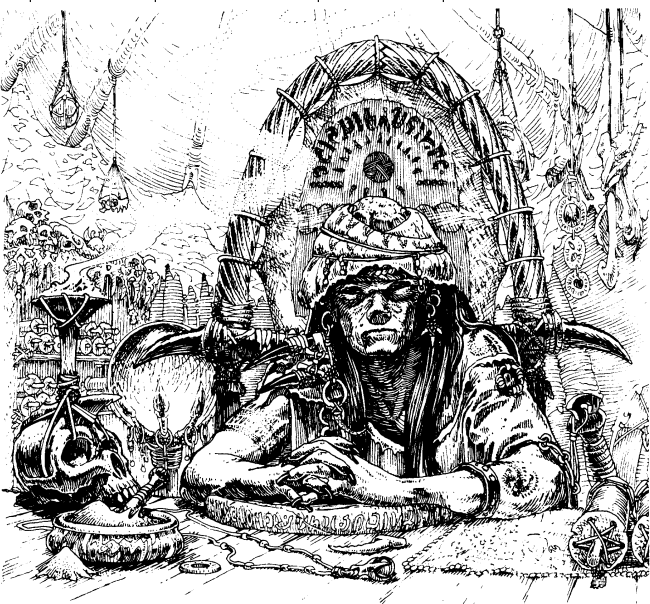
\includegraphics[width=\textwidth-2cm]{images/wizard-5.png}
\WOTC
\end{figure*}

\textbf{Bonus Languages:} A wizard may substitute Draconic for one of the bonus languages available to the character because of her race.

\textbf{Familiar:} A wizard can obtain a familiar. Doing so takes 24 hours and uses up magical materials that cost 100 ceramic pieces. A familiar is a magical beast that resembles a small animal and is unusually tough and intelligent. The creature serves as a companion and servant.

The wizard chooses the kind of familiar he gets. As the wizard advances in level, his familiar also increases in power.

If the familiar dies or is dismissed by the wizard, the wizard must attempt a DC 15 Fortitude saving throw. Failure means he loses 200 experience points per wizard level; success reduces the loss to one-half that amount. However, a wizard's experience point total can never go below 0 as the result of a familiar's demise or dismissal. A slain or dismissed familiar cannot be replaced for a year and day. A slain familiar can be raised from the dead just as a character can be, and it does not lose a level or a Constitution point when this happy event occurs.

A character with more than one class that grants a familiar may have only one familiar at a time.

\textbf{Scribe Scroll:} At 1st level, a wizard gains \feat{Scribe Scroll} as a bonus feat.

\textbf{Path:} At 1st level, a wizard must choose a philosophical path: preservation or defilement. This choice is not final. Preservers can defile and be corrupted, and defilers can get redemption.

\textit{Path Dexter:} Wizards who take this path are preservers. They master the balance of the arcane, casting spells with no collateral environmental damage.

Preservers learn one spell at each wizard level from abjuration or divination schools. They are drawn to protection and information spells.

\textit{Path Sinister:} This path is allowed only for nongood wizards. The wizards who take this path are defilers. With every spell cast, defilers take the life out of the plants and soil around them.

Defilers learn one spell at each wizard level from evocation or necromancy schools. They best utilize those darker and more destructive schools.

\textbf{Bonus Feats:} At 5th, 10th, 15th, and 20th level, a wizard gains a bonus feat. At each such opportunity, she can choose a metamagic feat, a raze feat, an item creation feat, or \feat{Spell Mastery}. The wizard must still meet all prerequisites for a bonus feat, including caster level minimums.

These bonus feats are in addition to the feat that a character of any class gets from advancing levels. The wizard is not limited to the categories of item creation feats, metamagic feats, or Spell Mastery when choosing these feats.

\textbf{Spellbooks:} A wizard must study her spellbook each day to prepare her spells. She cannot prepare any spell not recorded in her spellbook, except for read magic, which all wizards can prepare from memory.

A wizard begins play with a spellbook containing all 0-level wizard spells (except those from her prohibited school or schools, if any; see School Specialization, below) plus three 1st-level spells of your choice. For each point of Intelligence bonus the wizard has, the spellbook holds one additional 1st-level spell of your choice.

At each new wizard level, she gains three new spells of any spell level or levels that she can cast (based on her new wizard level) for her spellbook, one of which must be from her path's schools. At any time, a wizard can also add spells found in other wizards' spellbooks to her own.

\subsubsection{Familiars}
A familiar is a normal animal that gains new powers and becomes a magical beast when summoned to service by a wizard. It retains the appearance, Hit Dice, base attack bonus, base save bonuses, skills, and feats of the normal animal it once was, but it is treated as a magical beast instead of an animal for the purpose of any effect that depends on its type. Only a normal, unmodified animal may become a familiar. An animal companion cannot also function as a familiar.

A familiar also grants special abilities to its master, as given on the table below. These special abilities apply only when the master and familiar are within 1.5 kilometer of each other.

Levels of different classes that are entitled to familiars stack for the purpose of determining any familiar abilities that depend on the master's level.

\Table{Familiars}{l X}{
	\tableheader Familiar & \tableheader Special\\
	Bat & Master gains a +3 bonus on \skill{Listen} checks\\
	Cat & Master gains a +3 bonus on \skill{Move Silently} checks\\
	Dustgull & Master gains a +3 bonus on \skill{Spot} checks\\
	Hawk & Master gains a +3 bonus on \skill{Spot} checks in bright light\\
	Kes'trekel & Master gains a +2 bonus on Reflex saves\\
	Lizard & Master gains a +3 bonus on \skill{Climb} checks\\
	Owl & Master gains a +3 bonus on \skill{Spot} checks in shadows\\
	Rat & Master gains a +2 bonus on Fortitude saves\\
	Raven$\dagger$ & Master gains a +3 bonus on \skill{Appraise} checks\\
	Skyfish & Master gains a +3 bonus on \skill{Swim} checks\\
	Sygra & Master gains a +3 hit points\\
	Tiny viper & Master gains a +3 bonus on \skill{Bluff} checks\\
	% Toad & Master gains +3 hit points\\
	% Weasel & Master gains a +2 bonus on Reflex saves
	\rowcolor{white}
	\multicolumn{2}{p{\columnwidth}}{$\dagger$ A raven familiar can speak one language of its master's choice as a supernatural ability.}
}


\textbf{Familiar Basics:} Use the basic statistics for a creature of the familiar's kind, but make the following changes:

\textit{Hit Dice:} For the purpose of effects related to number of Hit Dice, use the master's character level or the familiar's normal HD total, whichever is higher.

\textit{Hit Points:} The familiar has one-half the master's total hit points (not including temporary hit points), rounded down, regardless of its actual Hit Dice.

\textit{Attacks:} Use the master's base attack bonus, as calculated from all his classes. Use the familiar's Dexterity or Strength modifier, whichever is greater, to get the familiar's melee attack bonus with natural weapons.

Damage equals that of a normal creature of the familiar's kind.

\textit{Saving Throws:} For each saving throw, use either the familiar's base save bonus (Fortitude +2, Reflex +2, Will +0) or the master's (as calculated from all his classes), whichever is better. The familiar uses its own ability modifiers to saves, and it doesn't share any of the other bonuses that the master might have on saves.

\textit{Skills:} For each skill in which either the master or the familiar has ranks, use either the normal skill ranks for an animal of that type or the master's skill ranks, whichever are better. In either case, the familiar uses its own ability modifiers. Regardless of a familiar's total skill modifiers, some skills may remain beyond the familiar's ability to use.

\Table{Familiar Progression}{b{1.4cm} Z{1.2cm} c X}{
	\tableheader Master Class Level & \tableheader Natural Armor Adj. & \tableheader Int & \tableheader Special\\
	1st--2nd & +1 & 6 & Alertness, improved evasion, share spells, empathic link\\
	3rd--4th & +2 & 7 & Deliver touch spells\\
	5th--6th & +3 & 8 & Speak with master\\
	7th--8th & +4 & 9 & Speak with animals of its kind\\
	9th--10th & +5 & 10 & \\
	11th--12th & +6 & 11 & Spell resistance\\
	13th--14th & +7 & 12 & Scry on familiar\\
	15th--16th & +8 & 13 & \\
	17th--18th & +9 & 14 & \\
	19th--20th & +10 & 15 &
}

\textbf{Familiar Ability Descriptions:} All familiars have special abilities (or impart abilities to their masters) depending on the master's combined level in classes that grant familiars, as shown on the table above. The abilities given on the table are cumulative.

\textit{Natural Armor Adj.:} The number noted here is an improvement to the familiar's existing natural armor bonus.

\textit{Int:} The familiar's Intelligence score.

\textit{Alertness (Ex):} While a familiar is within arm's reach, the master gains the Alertness feat.

\textit{Improved Evasion (Ex):} When subjected to an attack that normally allows a Reflex saving throw for half damage, a familiar takes no damage if it makes a successful saving throw and half damage even if the saving throw fails.

\textit{Share Spells:} At the master's option, he may have any spell (but not any spell-like ability) he casts on himself also affect his familiar. The familiar must be within 1.5 meter at the time of casting to receive the benefit.

If the spell or effect has a duration other than instantaneous, it stops affecting the familiar if it moves farther than 1.5 meter away and will not affect the familiar again even if it returns to the master before the duration expires. Additionally, the master may cast a spell with a target of ``You'' on his familiar (as a touch range spell) instead of on himself.

A master and his familiar can share spells even if the spells normally do not affect creatures of the familiar's type (magical beast).

\textit{Empathic Link (Su):} The master has an empathic link with his familiar out to a distance of up to 1.5 kilometer. The master cannot see through the familiar's eyes, but they can communicate empathically. Because of the limited nature of the link, only general emotional content can be communicated.

Because of this empathic link, the master has the same connection to an item or place that his familiar does.

\textit{Deliver Touch Spells (Su):} If the master is 3rd level or higher, a familiar can deliver touch spells for him. If the master and the familiar are in contact at the time the master casts a touch spell, he can designate his familiar as the ``toucher.'' The familiar can then deliver the touch spell just as the master could. As usual, if the master casts another spell before the touch is delivered, the touch spell dissipates.

\textit{Speak with Master (Ex):} If the master is 5th level or higher, a familiar and the master can communicate verbally as if they were using a common language. Other creatures do not understand the communication without magical help.

\textit{Speak with Animals of Its Kind (Ex):} If the master is 7th level or higher, a familiar can communicate with animals of approximately the same kind as itself (including dire varieties): bats with bats, rats with rodents, cats with felines, hawks and owls and ravens with birds, lizards and snakes with reptiles, toads with amphibians, weasels with similar creatures (weasels, minks, polecats, ermines, skunks, wolverines, and badgers). Such communication is limited by the intelligence of the conversing creatures.

\textit{Spell Resistance (Ex):} If the master is 11th level or higher, a familiar gains spell resistance equal to the master's level + 5. To affect the familiar with a spell, another spellcaster must get a result on a caster level check (1d20 + caster level) that equals or exceeds the familiar's spell resistance.

\textit{Scry on Familiar (Sp):} If the master is 13th level or higher, he may scry on his familiar (as if casting the scrying spell) once per day.

\subsubsection{School Specialization}
A school is one of eight groupings of spells, each defined by a common theme. If desired, a wizard may specialize in one school of magic (see below). Specialization allows a wizard to cast extra spells from her chosen school, but she then never learns to cast spells from some other schools.

A specialist wizard can prepare one additional spell of her specialty school per spell level each day. She also gains a +2 bonus on \skill{Spellcraft} checks to learn the spells of her chosen school.

The wizard must choose whether to specialize and, if she does so, choose her specialty at 1st level. At this time, she must also give up two other schools of magic (unless she chooses to specialize in divination; see below), which become her prohibited schools.

A wizard can never give up divination to fulfill this requirement.

Spells of the prohibited school or schools are not available to the wizard, and she can't even cast such spells from scrolls or fire them from wands. She may not change either her specialization or her prohibited schools later.

The eight schools of arcane magic are abjuration, conjuration, divination, enchantment, evocation, illusion, necromancy, and transmutation.

Spells that do not fall into any of these schools are called universal spells.

\begin{figure}[t!]
\centering
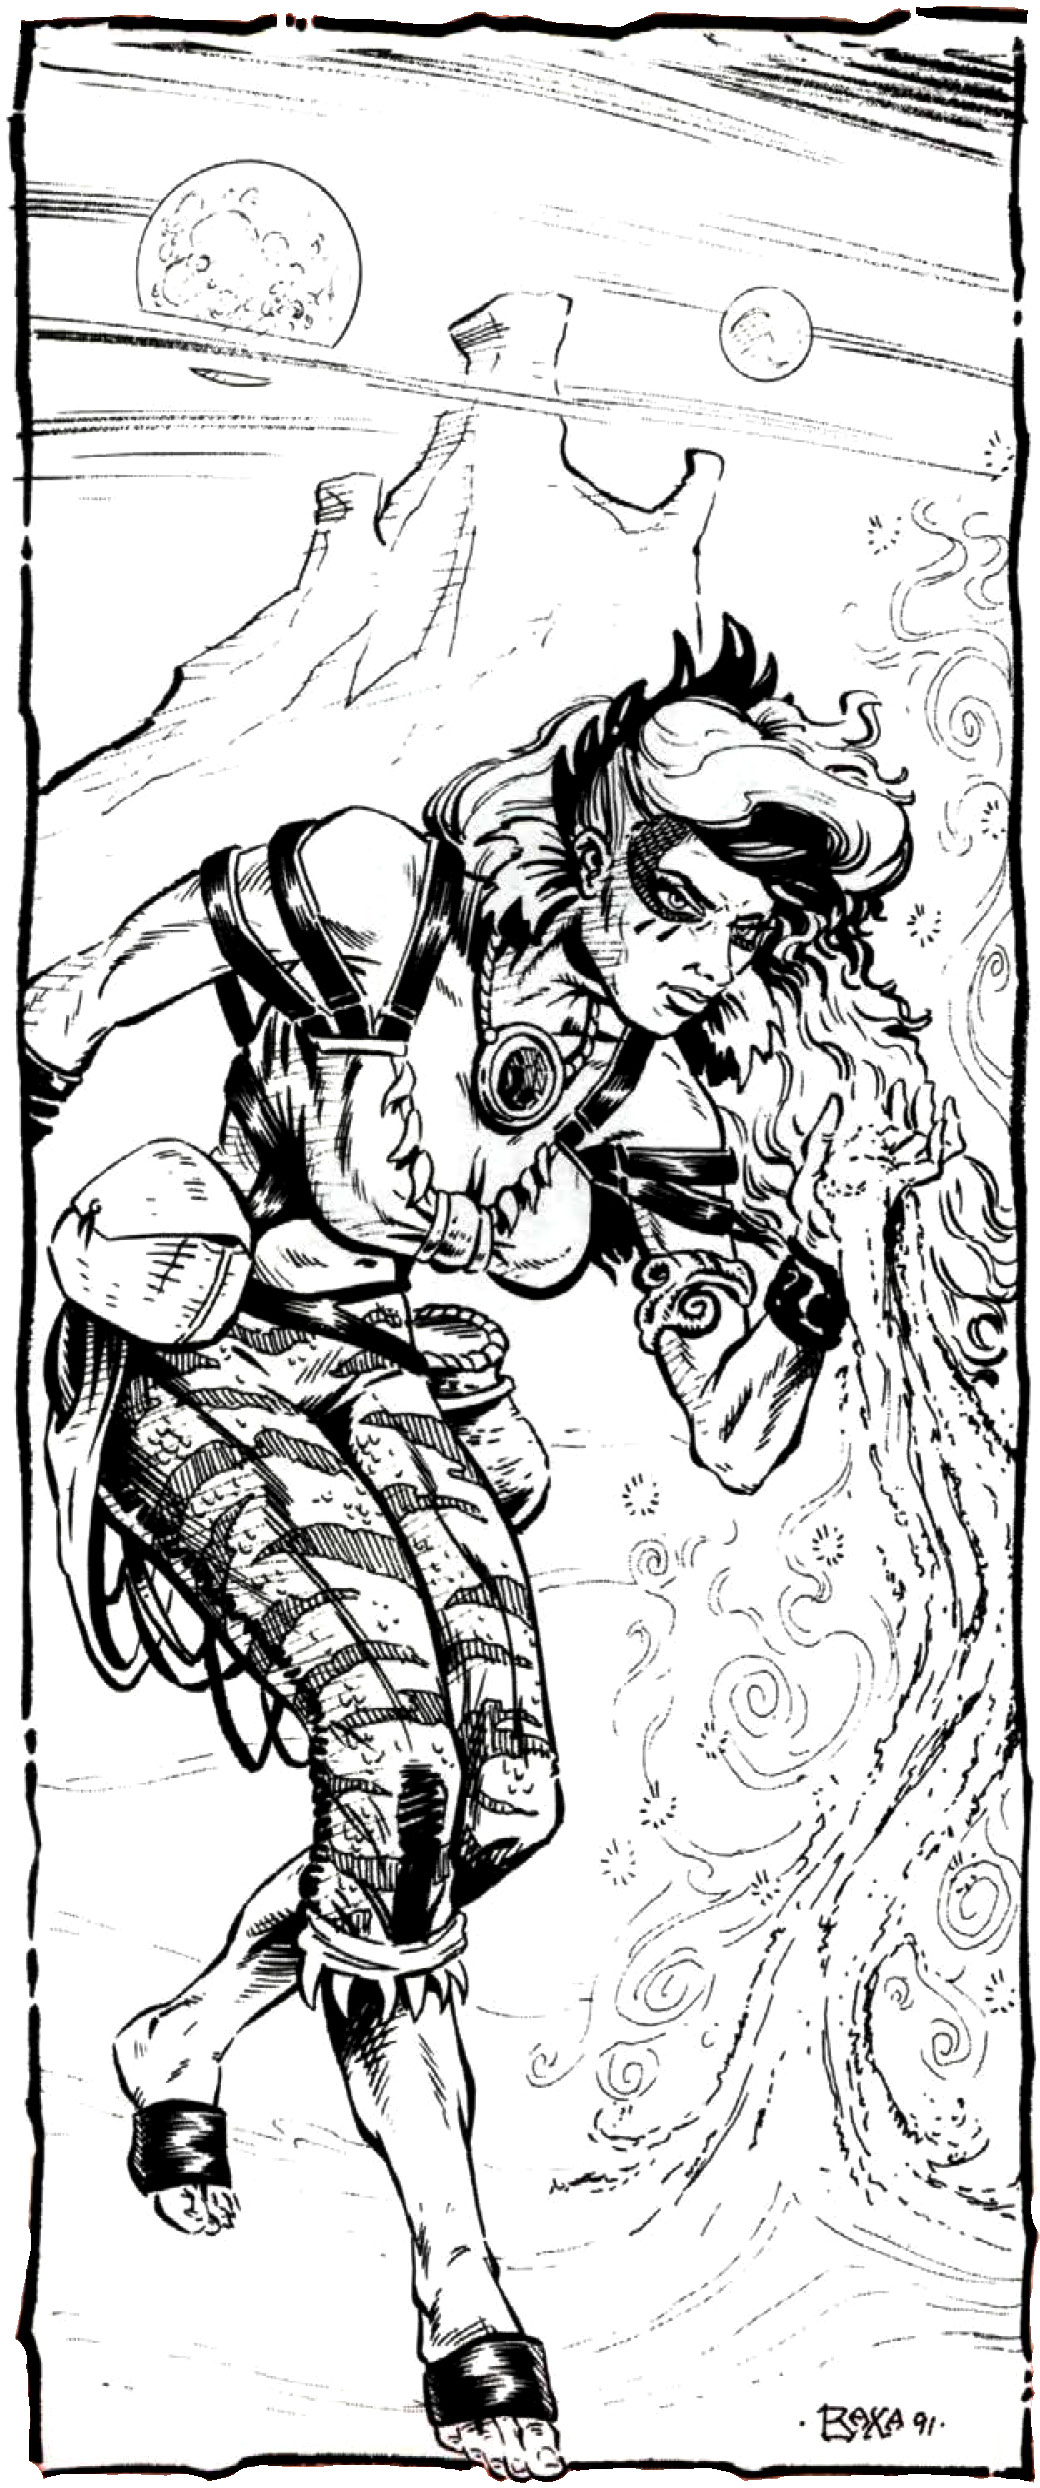
\includegraphics[width=\columnwidth]{images/wizard-2.png}
\WOTC
\end{figure}


\textbf{Abjuration:} Spells that protect, block, or banish. An abjuration specialist is called an abjurer.

\textbf{Conjuration:} Spells that bring creatures or materials to the caster. A conjuration specialist is called a conjurer.

\textbf{Divination:} Spells that reveal information. A divination specialist is called a diviner. Unlike the other specialists, a diviner must give up only one other school.

\textbf{Enchantment:} Spells that imbue the recipient with some property or grant the caster power over another being. An enchantment specialist is called an enchanter.

\textbf{Evocation:} Spells that manipulate energy or create something from nothing. An evocation specialist is called an evoker.

\textbf{Illusion:} Spells that alter perception or create false images. An illusion specialist is called an illusionist.

\textbf{Necromancy:} Spells that manipulate, create, or destroy life or life force. A necromancy specialist is called a necromancer.

\textbf{Transmutation:} Spells that transform the recipient physically or change its properties in a more subtle way. A transmutation specialist is called a transmuter.

\textbf{Universal:} Not a school, but a category for spells that all wizards can learn. A wizard cannot select universal as a specialty school or as a prohibited school. Only a limited number of spells fall into this category.

\subsubsection{Ex-Defilers}
Arcane casters who defile must roll a Will save DC 10 + spell level + amount of times previously defiled. Failing this save, they become defilers. Preservers succeeding the save lose their preserver status and become tainted. For more rules on defiling, see \chapref{Magic}.

Tainted wizards are not defilers, but risk becoming so. Tainted wizards may seek redemption from a druid. The druid, if willing and able, can cast a \spell{conversion} spell on the tainted wizard, restoring her preserver status (reset the number of times defiled to zero). The wizard loses 100 XP per arcane spellcaster level.

Defilers can also seek redemption, but lose 1,000 XP per arcane spellcaster level. Usually the defiler must undertake a quest or otherwise demonstrate a true willingness to redeem herself before the druid casts the \spell{conversion} spell.


\subsection{Playing a Wizard}
You are a master of arcane secrets. You have learned, either on your own, or from someone in your family, how to draw on vegetable life in order to power your spells. But such power comes with a caveat, arcane magic is universally feared and hated. You might be inclined to see conspiracies and enemies where none exist, so accustomed are you to being hunted and persecuted by the general populace and sorcerer-king's templars because of your talents.

Mostly, you adventure to perfect your understanding and mastery of magic. You likely prefer endeavors that allow frequent use of your abilities, or those that promise access to ancient lore. You might have personal goals as well, and it's not uncommon for an Athasian wizard to adventure for the sake of riches, power, eternal life, or any other ``standard'' adventurer motive.

\subsubsection{Religion}
Wizards frequently find themselves at odds with the elemental forces that grant clerics their powers, though it is not unheard of for preservers to forge an Elemental Pact. Some preservers might also associate themselves with the assorted Spirits of the Land. Since they understand the sorcerer-kings to simply be exceptionally advanced wizards, they are not given to revering their kings, as some of their more naive brothers are known to do.

\subsubsection{Other Classes}
Wizards have a difficult time relating to most of the other classes. Templars and wizards are, in most cases, deadly enemies across an irreconcilable gap---the exception is those rare defilers in the employ of the sorcerer-kings. Likewise, druids are likely to consider any wizard a potential defiler, and would turn on a companion the moment this suspicion is confirmed. Due to their similar, ``underground'' nature, wizards feel a certain respect for bards. While preservers enjoy an uneasy truce with the elemental powers, defilers and paraelemental clerics tend get along quite well.

\subsubsection{Combat}
Athasian wizards stay back from melee and use your spells to either destroy your enemies or enhance your companion's abilities. Secrecy is a major component, even more so if you are a defiler. Casting even of the simplest of arcane spells can focus all of your enemies' attention to you, even more so if you are a defiler. Be prepared to run of fly away in such cases.

\subsubsection{Advancement}
Continuing your advancement as a wizard requires a substantial amount of time and effort. You must procure and study arcane texts, not merely to learn new spells, but to comprehend the nature of what you do.

When you not studying, you are practicing, training your mind and your body to channel ever greater amounts of life force.

As you start to progress in the class, consider studying other sources of arcane energy, such as the Black, the Gray, and the Cerulean, since those would remove your dependency on vegetable life around you. Most wizards seek to become some day as powerful as Dragon Kings or the fabled winged creature the Urikite known as Korgunard turned into.

Mechanically, you should increase your Intelligence and Charisma as you attain levels. Beyond this, focus on feats (such as Path Dexter or Path Sinister) and skills that enhance your spells and provide you the abilities you need to remain in secrecy, mainly Bluff and Disguise.

\vskip3cm

\subsection{Starting Packages}
\subsubsection{The Dexter}
Pterran Wizard

\textbf{Ability Scores:} Str 8, Dex 10, Con 10, Int 15, Wis 16, Cha 15.

\textbf{Skills:} \skill{Bluff}, \skill{Concentration}, \skill{Disguise}, \skill{Knowledge} (arcana), \skill{Knowledge} (local), \skill{Spellcraft}.

\textbf{Languages:} Common, Elven, Saurian.

\textbf{Feat:} \feat{Path Dexter}.

\textbf{Weapons:} Dagger (1d4/19--20, 3 m)

Light crossbow with 20 bolts (1d6/$\times$3, 18 m).

\textbf{Armor:} Padded (+1 AC).

\textbf{Other Gear:} Standard adventurer's kit, spell

component pouch, 31 cp.

\subsubsection{The Concurrent}
Human Wizard

\textbf{Ability Scores:} Str 8, Dex 13, Con 10, Int 15, Wis 14, Cha 12.

\textbf{Skills:} \skill{Bluff}, \skill{Concentration}, \skill{Decipher Script}, \skill{Disguise}, \skill{Knowledge} (arcana), \skill{Knowledge} (local), \skill{Spellcraft}.

\textbf{Languages:} City language, Common, Elven.

\textbf{Feat:} \feat{Alertness}, \feat{Improved Initiative}.

\textbf{Weapons:} Dagger (1d4/19--20, 3 m)

Light crossbow with 20 bolts (1d6/$\times$3, 18 m).

\textbf{Armor:} Padded (+1 AC).

\textbf{Other Gear:} Standard adventurer's kit, spell component pouch, 31 cp.

\subsubsection{The Sinister}
Elf Wizard

\textbf{Ability Scores:} Str 10, Dex 16, Con 10, Int 15, Wis 13, Cha 8.

\textbf{Skills:} \skill{Bluff}, \skill{Concentration}, \skill{Knowledge} (arcana), \skill{Knowledge} (local), \skill{Spellcraft}.

\textbf{Languages:} City language, Common, Elven.

\textbf{Feat:} \feat{Destructive Raze}.

\textbf{Weapons:} Dagger (1d4/19--20, 3 m)

Light crossbow with 20 bolts (1d6/$\times$3, 18 m).

\textbf{Armor:} Padded (+1 AC).

\textbf{Other Gear:} Standard adventurer's kit, spell component pouch, 31 cp.

\subsection{Wizards on Athas}
\Quote{'Witch!' they chanted. 'Kill the witch!' By the time the soldiers woke, the crowd had finished her off, and worse. The mage's death did not satisfy the mob; her body suffered much more. When the mul leader shouted, 'we'll take her and burn her!' they cheered. For the only time in my life I saw a crowd cheer for Kalak's guards. For the first time I saw wizard's magic. For the first time I understood its peril.}{Manok, Tyrian wizard}

On Athas, the energy for wizardly magic doesn't come from some extradimensional source as it does on other worlds, but from the living environment itself. It provides great power to those who can gather and shape it, though the cost to Athas can be beyond measure.

In recent times wizards have emerged who have learned to draw energy from alternate sources that have no impact on the environment, see Prestige Class Appendix I for more information.

\subsubsection{Daily Life}
The kinds of activities that appeal to wizards depend largely on their alignment and energy gathering method. Good wizards spend their time trying to restore the devastation of Athas and fighting against the forces of the sorcerer-kings, while evil preservers of defilers are interested in helping themselves.

When not adventuring, Athasian wizards spend the majority of their time in study and in hiding. Much like wizards from other settings, they must constantly research new spells and study ancient arcane texts so thoroughly that they have little time to devote to other endeavors.

\subsubsection{Notables}
Usually wizards try to stay incognito for as long as they can, since their survival depends on it. However, a few wizards manage to become quite famous on Athas. Royal defilers and arena necromancers, such as Dote Mal Payn, even though hated by the general populace are sponsored by their sorcerer-kings and do not need to hide their skills. Sadira of Tyr was made famous for her contribution in killing King Kalak the Tyrant and the Dragon, and she has become the first (and maybe the only one) wizard able to tap into the power of the crimson sun. The most famous wizards are the Dragon Kings, of course, who can destroy both plant life and living creatures to power their spells.

\subsubsection{Organizations}
Wizardly magic on Athas isn't as codified and formal as it is in other campaign settings. For example, there are no academies or colleges for teaching the wizardly arts. Instead, a wizard-in-training must find a teacher, which isn't very easy in a world where wizards must hide their profession in order to survive. For protection from nearly universal hatred, the good wizards of Athas and their allies have formed secret societies, collectively known as the Veiled Alliance.

However, each city-state holds a different Alliance, they do not cooperate, and they share no leaders. Members of one Alliance do not automatically become members of another. At best, the different groups respect each other, and may offer courtesy assistance to a foreign member who arrives in town.

Defilers don't usually organize together, but they often join organizations, especially Merchant Houses and raiding tribes.

\subsubsection{NPC Reactions}
Arcane magic in Athas is viewed as more dangerous and destructive than helpful, so general NPC attitudes towards someone suspected to be a wizard range from indifferent to unfriendly. If a NPC actually witness a wizard drawing magical energy or casting a spell, the resultant fear and hatred shifts the NPC's attitude toward hostile.

Arcane magic is banned in almost all city-states; Tyr has unbanned it after FY 0 after Kalak was killed and Kurn has no qualms about preserving magic. Templars constantly patrol the streets searching for wizards and arcane items.

\subsubsection{Wizard Lore}

Characters with ranks in \skill{Knowledge} (arcana) can research wizards to learn more about them. When a character makes a skill check, read or paraphrase the following, including the information from lower DCs.

\textbf{DC 10:} Wizards are magic users that fuel their spells with plant life.

\textbf{DC 15:} A wizard can be either a defiler or a preserver. Only the first destroys the land when casting a spell. Defilers can increase the potency of their spells by destructing larger areas of vegetation than necessary.

\textbf{DC 20:} Some say that other wizards have developed a way to draw energy from other source than plants.


\begin{figure}[b!]
\centering
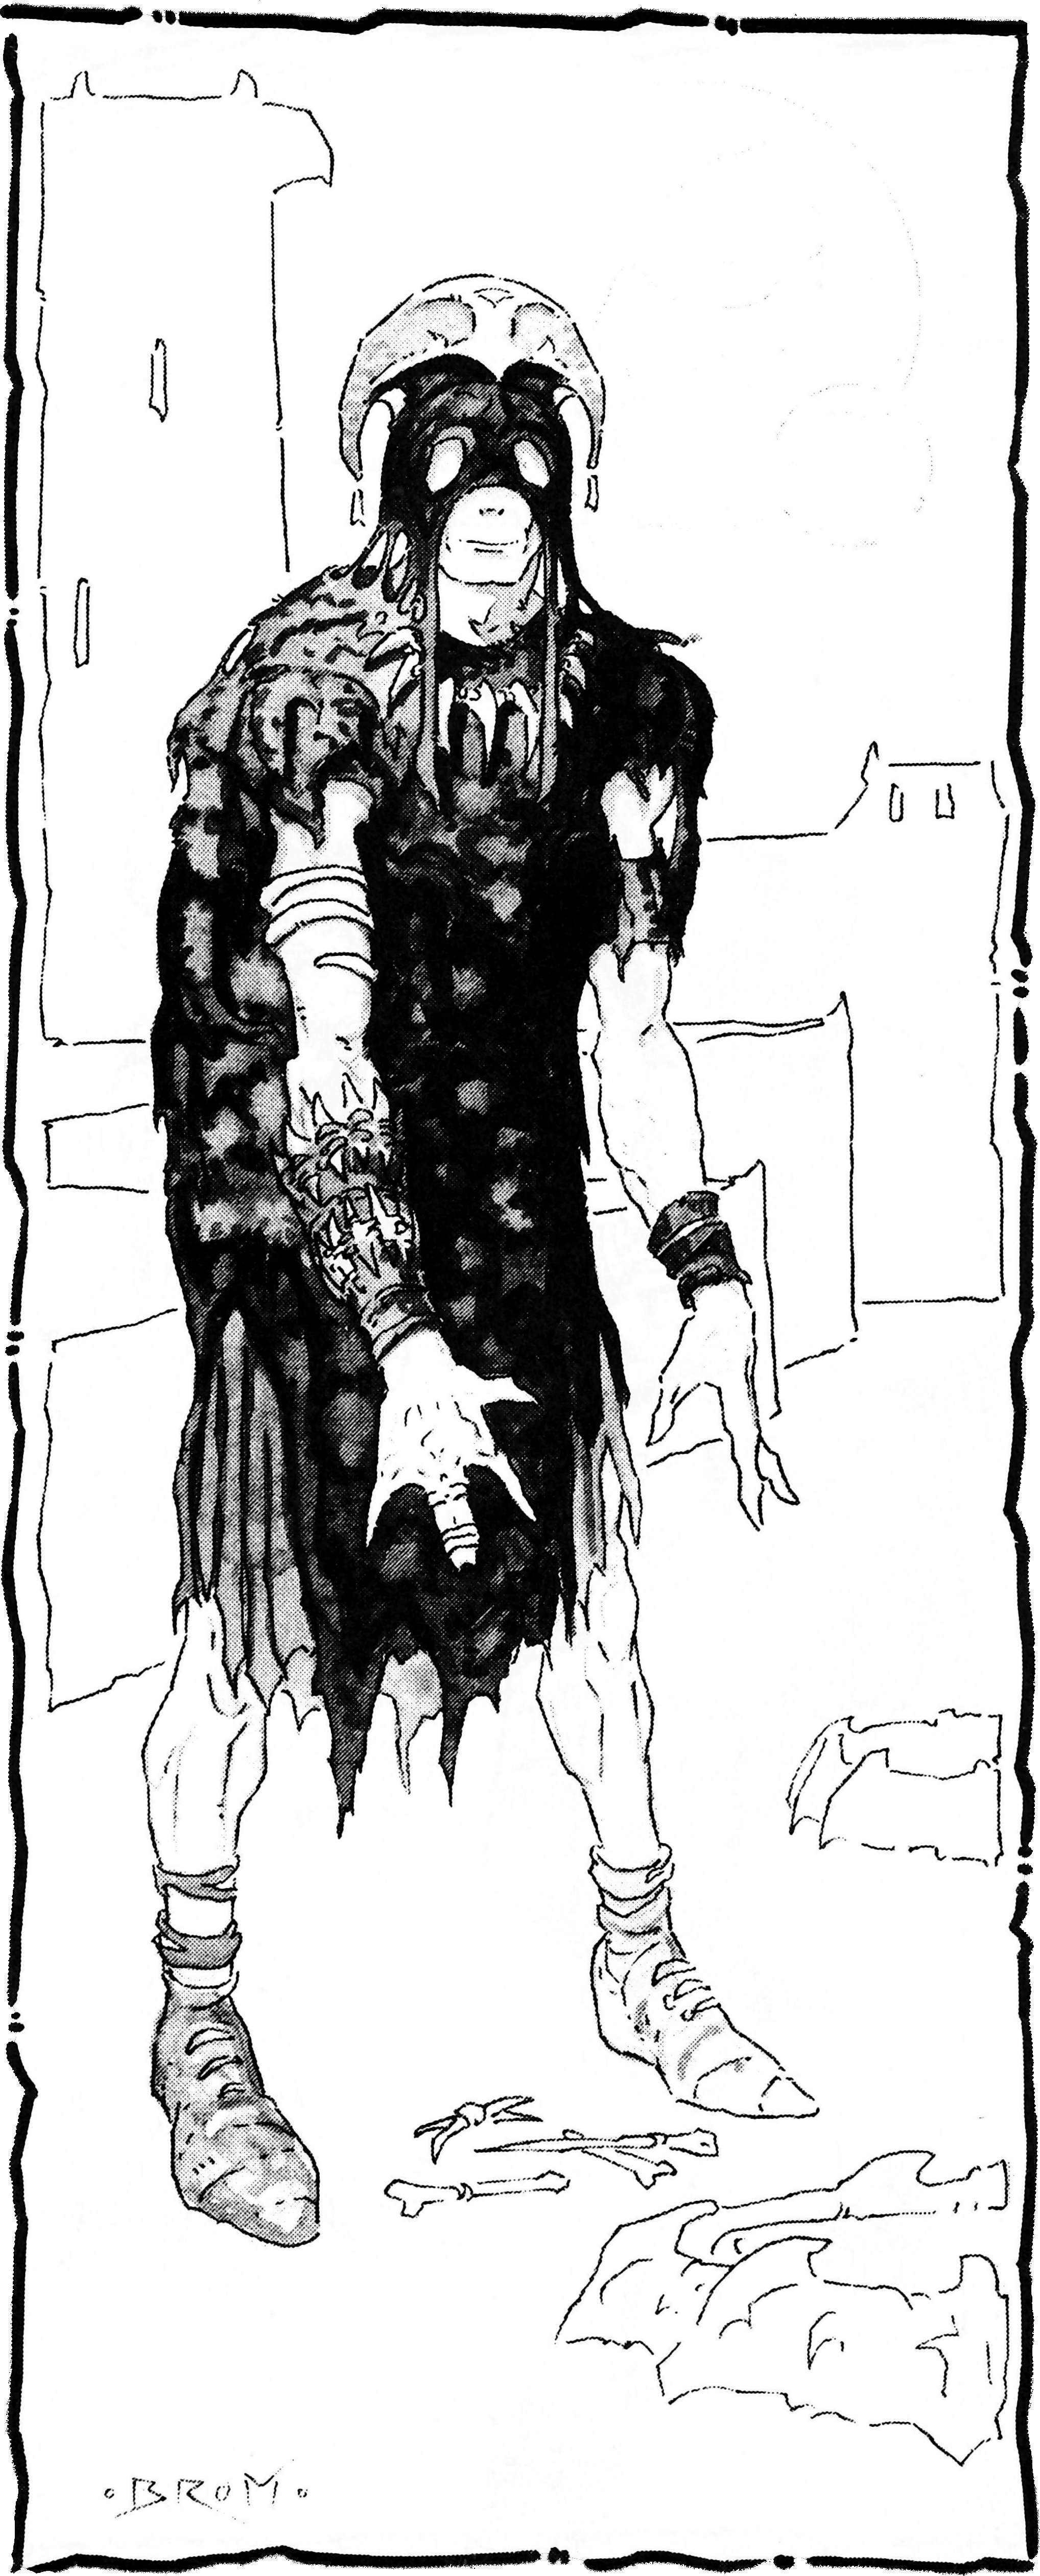
\includegraphics[width=\columnwidth]{images/wiz-1.png}
\WOTC
\end{figure}
\section{Multiclass Characters}
A character may add new classes as he or she progresses in level, thus becoming a multiclass character. The class abilities from a character's different classes combine to determine a multiclass character's overall abilities. Multiclassing improves a character's versatility at the expense of focus.

\subsection{Prerequisites}
To qualify for a new class, you must meet the ability score prerequisites for both your current class and your new one, as shown in \tabref{Multiclassing Prerequisites}. For example, a barbarian who decides to multiclass into the druid class must have Wisdom score of 15 or higher, and both Strength and Constitution scores of 13 or higher. Without the full training that a beginning character receives, you must be a quick study in your new class, having a natural aptitude that is reflected by higher-than-average ability scores.

\Table{Multiclassing Prerequisites}{lL}{
\tableheader Class & \tableheader Ability Score Minimum \\
Barbarian       & Strength 13, Constitution 13 \\
Bard            & Charisma 13, Dexterity or Intelligence 13 \\
Cleric          & Wisdom 13, Charisma 13 \\
Druid           & Wisdom 15 \\
Fighter         & Constitution 13, Strength or Dexterity 13 \\
Gladiator       & Strength 13, Intelligence or Charisma 13 \\
Psion           & Wisdom 13, Constitution or Intelligence 13 \\
% Psychic Warrior & Strength or Dexterity 13, Wisdom 13 \\
Ranger          & Wisdom 13, Strength or Dexterity 13 \\
Scout           & Dexterity 13, Strength or Wisdom 13 \\
Templar         & Wisdom 13, Charisma 13 \\
Thief           & Dexterity 13, Intelligence or Charisma 13 \\
% Wilder          & Charisma 15 \\
Wizard          & Intelligence 15 \\
}

\subsection{Class And Level Features}
As a general rule, the abilities of a multiclass character are the sum of the abilities of each of the character's classes.

\textbf{Level:} ``Character level'' is a character's total number of levels. It is used to determine when feats and ability score boosts are gained.

``Class level'' is a character's level in a particular class. For a character whose levels are all in the same class, character level and class level are the same.

\textbf{Hit Points:} A character gains hit points from each class as his or her class level increases, adding the new hit points to the previous total.

\textbf{Base Attack Bonus:} Add the base attack bonuses acquired for each class to get the character's base attack bonus. A resulting value of +6 or higher provides the character with multiple attacks.

\textbf{Saving Throws:} Add the base save bonuses for each class together.

\textbf{Skills:} If a skill is a class skill for any of a multiclass character's classes, then character level determines a skill's maximum rank. (The maximum rank for a class skill is 3 + character level.)

If a skill is not a class skill for any of a multiclass character's classes, the maximum rank for that skill is one-half the maximum for a class skill.

\textbf{Class Features:} A multiclass character gets all the class features of all his or her classes but must also suffer the consequences of the special restrictions of all his or her classes.

In the special case of turning undead, both clerics and experienced templars have the same ability. If the character's templar level is 4th or higher, her effective turning level is her cleric level plus her templar level.

In the special case of uncanny dodge, experienced barbarians, experienced gladiators, experienced scouts, and experienced thieves have the same ability. When a barbarian/rogue would gain uncanny dodge a second time (for her second class), she instead gains improved uncanny dodge, if she does not already have it. Her barbarian and rogue levels stack to determine the rogue level an attacker needs to flank her.

\textbf{Feats:} A multiclass character gains feats based on character levels, regardless of individual class level

\textbf{Ability Increases:} A multiclass character gains ability score increases based on character level, regardless of individual class level.

\textbf{Spells:} The character gains spells from all of his or her spellcasting classes and keeps a separate spell list for each class. If a spell's effect is based on the class level of the caster, the player must keep track of which class's spell list the character is casting the spell from.

\textbf{Power Points:} If you have levels in more than one psionic class, you combine your power points from each class to make up your reserve. You can use these power points to manifest powers from any psionic class you have.

While you maintain a single reserve of power points from your class, race, and feat selections, you are still limited by the manifester level you have achieved with each power you know.

\section{Alternative Class Features}
Choosing a class fixes key aspects of a character: their role, their abilities, and their attack and save bonuses. However, you can change a class feature to provide a new experience. Variant versions of several of class features are presented below. If you prefer the variant to the standard class feature, ask your game master if he approves of your swapping out your class feature for the variant version.

These alternative class features can exist side by side with the standard class features---some bards might work alone while their comrades favor having contacts all over Athas---or can completely replace the standard features. The balance between the standard class features and the alternative features is up to the game master.

The description of alternative class features is the following.

\subsubsection{Alternative Class Feature Name}
A general description of the ability.

\textbf{Special Requirement:} Any special requirements that you must meet before selecting the alternative class feature. Many of the alternative class features described here require ranks of a skill. Since skill ranks are purchased before class features are selected, you can meet this requirement at the same level that you gain the alternative class feature.

\textbf{Level:} The alternative class feature can be selected only at this level. In some cases, different levels might be given for different classes.

\textbf{Replaces:} The ability that you must sacrifice to gain the alternative class feature.

\textbf{Benefit:} The mechanical effects of the new ability.


\subsection{Bard}
Athasian bards are city guides, traders, translators, or even assassins. They fill their role in society with their social skills and scoundrel minds.

\AlternateClassFeature{Contact}
{Instead of relying on their own wits like a traditional bard, a \emph{draqoman} relies on the help of others more capable in specific matters. Draqomen serve as guides and translators for newcomers to the cities. Local laws and customs vary by location, and a local resident who knows the city like the back of his hand and can call in a favor if necessary is definitely worth his pay. A draqoman will usually be loyal as long as he is paid and fed well. Mistreat your draqoman and you will soon find yourself on the wrong end of someone's blade or in the prisons run by the templars.}
{\skill{Diplomacy} 2 ranks, \skill{Gather Information} 4 ranks, \skill{Knowledge} (local) 4 ranks.}
{6th, 11th, and 16th.}
{You do not gain quick thinking, or its improvements at 11th and 16th levels.}
{
	You gain the trust of two non-player characters he can rely on when the time comes. You can ask for a favor once per week per contact. Contacts come in three varieties, one of which you must choose: influence contacts, skill contacts, and trade contacts (see \hyperref[sec:contacts]{Contacts}).

	You gain one additional contact every three levels thereafter (3 at 9th, 4 at 12th, 5 at 15th, and 6 at 18th level).
}
\AlternateClassFeature{Procurer}
{To all outward appearances, procurers seem to be everyday elf traders. They conduct their thefts in secret, using normal trading practices to cover their filching activities. These elves usually work for elven merchant houses, filling the market stalls with goods stolen from other merchants, nobles, free citizens, templars, and even the sorcerer-kings.}
{Elf or half-elf.}
{4th, 8th, 12th, 16th, or 20th.}
{You do not gain a trade secret.}
{
	You gain +5 in \skill{Search} checks to find secret doors, and if you pass within 1.5 meter of a secret door, you are entitled to a \skill{Search} check to notice it as if the character was actively looking for it.
}


\subsection{Fighter}
The nomad elves need fighters who can keep up with the tribe, maybe even lead it one day, while The Kreen Empire breeds a stronger strain to defend it against the humanoid threat. No matter the reason, Each culture and race has reached a way to specialize their fighters to survive the dangers of Athas.

\AlternateClassFeature{Reckless}
{The eagle knights are among the most brutal and fanatical Draji warriors. They are more than willing to charge headfirst into battle for the glory of Draj and their god-king.}
{Must be trained by the Draji army.}
{11th.}
{You do not gain martial prowess.}
{
	When using the attack or full attack option, you can subtract a number from his Armor Class and add this number to damage inflicted on successful attacks. This number may not exceed your base attack bonus. The Armor Class penalty and damage bonus last until the your next standard action.
}
\AlternateClassFeature{Savage Hunter}
{The savage hunter is the most common elf warrior type, serving as both a tribal defender and an important food provider. Respected by others of the tribe, the savage hunter uses the same skills to hunt prey and to fight outsiders and other threats to the tribe. The ways of the city-states are alien to these wilderness warriors, for they are only at home in the wastes when on a hunt.}
{Elf or half-elf.}
{1st.}
{You do not gain a bonus feat.}
{
	You gain \feat{Track} as a bonus feat. You add \skill{Survival} to your fighter class skills.
}

\AlternateClassFeature{Tik-Tik}
{Larger and less dexterous than most other kreen, the ``hunter-of-hunters'' guards the weaker members of the pack. In dangerous territory, Tik-Tik rarely hunt, unless the pack's normal hunters are spread too thinly or have been incapacitated by enemies.}
{Thri-kreen.}
{1st.}
{You do not gain a bonus feat.}
{
	Your natural armor bonus increases by 1 (+3 total). You add \skill{Survival} to your fighter class skills.
}


\subsection{Gladiator}
The city-state arenas are packed with all kinds of gladiators, from those who fight only with the heaviest piece of armor available to those who are able to optimize their flexibility and movement with what they have.

\AlternateClassFeature{Flexibility Adjustment}
{These gladiators adjust their armor to improve their reflex capabilities instead of increasing the area it protects.}
{}
{5th, 10th, 15th, and 20th.}
{You do not gain armor optimization, or its improvements at 10th, 15th, and 20th levels.}
{
	You improve the maximum Dexterity bonus and reduce the armor check penalty by 1, whenever you are wearing any armor you are proficient with.

	At every five levels thereafter, the improvement increases by 1 (2 at 10th, 3 at 15th, and 4 at 20th level).
}
\AlternateClassFeature{Lighten Load}
{By changing slightly the armor to their own bodies, these gladiators can move faster with a heavier armor.}
{}
{5th.}
{You do not gain the first armor optimization.}
{
	You treat the medium armor as light armor. You also reduce the armor check penalty by 1, whenever you are wearing any armor you are proficient with.
}


\subsection{Psion}
The Way is taught differently throughout the Tablelands. Urban folk teach, willingly or not, about having a friendship network in their cities. Tribal people, without formal study, have devised a ritual to aid their psychic abilities. The Kreen uses their Will to overcome the difference between their mind and the humanoid ones.

\AlternateClassFeature{Contact}
{The cities of Athas are filled with intrigue, treachery, and double-dealing. In this setting, information is a weapon that may be wielded against one's enemies. The auditor's job description ranges from information broker to psionic assassin. In most cities, the templars have auditors working for them. Other auditors are members of the Veiled Alliance, criminal gangs, or are employed by the merchant dynasties.}
{\skill{Diplomacy} 2 ranks, \skill{Gather Information} 4 ranks, \skill{Knowledge} (local) 4 ranks.}
{1st, 5th, 10th, 15th, and 20th.}
{You do not gain any bonus feat.}
{
	You gain the trust of a non-player character he can rely on when the time comes. You can ask for a favor once per week per contact. Contacts come in three varieties, one of which you must choose: influence contacts, skill contacts, and trade contacts (see \hyperref[sec:contacts]{Contacts}).

	You gain one additional use of contact at 5th level and every four levels thereafter (2 contacts at 5th, 3 at 9th, 4 at 13th, 5 at 17th).
}
\AlternateClassFeature{Psionic Ritual}
{Bereft of formal training in the Way, psionically talented individuals from the tribal and nomadic peoples of the Tablelands and beyond must make do with their own understanding of the psionic arts. Seen by formally trained psions as an aberration of proper psionic practice, these self trained individuals can sometimes produce effects that leave their detractors speechless.}
{\skill{Profession} (herbalist) 8 ranks, \skill{Survival} 6 ranks.}
{10th.}
{You do not gain a bonus feat.}
{
	Once per day, you can perform such a ritual to temporarily increase your Will. Each psionic ritual is unique, being of your own design, but all take one hour to complete and require a DC 20 \skill{Concentration} check. If the ritual is successful, you gain 1d4+1 temporary power points over and above your normal maximum. These power points remain available for one day or until they are used.
}

\AlternateClassFeature{Tekchakak}
{The tekchakak is devoted to the preservation and prosperity of clutch and pack. These psions use their abilities to support their clutchmates and packmates, helping to find prey and to defend compatriots against raiders and predators. Within a thri-kreen pack, the tekchakak offers advice, guidance, and teaching in addition to active support through their psionic abilities.}
{Thri-kreen.}
{1st.}
{You do not gain a bonus feat.}
{
	You no longer have alien mind (see \chapref{Character Races}). You add \skill{Survival} to your psion class skills.
}


\subsection{Ranger}
Protectors of the wastelands, rangers are lone survivalists who help those in need. More often than not, they aim their hatred towards those who threaten their tribes.

\AlternateClassFeature{Elf Favored Enemy}
{These insectoid hunters love the taste of elf flesh, and they prey upon the desert runners whenever the  opportunity presents itself. In order to combat the threat posed by the fast, strong, and cunning thri-kreen, a special class of desert runner has developed---the thri-kreen slayer.}
{Elf or half-elf.}
{1st.}
{You do not gain favored enemy.}
{
	You narrow down your choice of favored enemy to thri-kreen. You gain a +3 bonus on \skill{Hide}, \skill{Listen}, \skill{Move Silently}, \skill{Spot}, and \skill{Survival} checks when using these skills against creatures of this race. Likewise, you get a +3 bonus on weapon damage rolls against such creatures.

	Each time you gain a new favored enemy and you choose to increase your bonus against thri-kreen, it increases by 3.
}
\AlternateClassFeature{Psionic Hunter}
{The tablelands are filled with psionic creatures, so much so that psionic abilities are expected from everyone in Athas. Most rangers do not concern with this common capabilities, but some are more interested on what a creature does. These rangers learn to identify psionic signs and make it their business to combat those who use psionic powers in opposition to their goals.}
{\skill{Knowledge} (psionic) 2 ranks.}
{1st.}
{You do not gain favored enemy.}
{
	You gain favored enemy (psionicists). This feature works just like the favored enemy ability. The bonuses granted apply to any character capable of manifesting psionic powers (but not psi-like abilities).
}
% \AlternateClassFeature{Salvage}
% {The kik has fully turned away from the life as a hunter and instead embraced the life of a raider, known in the language of the thri-kreen as a kik. The kik are in many ways more barbaric then the average kreen who roam the Tablelands, though they are not as feral as their cousins the trin.}
% {Thri-kreen, \skill{Search} 5 ranks, \skill{Survival} 5 ranks.}
% {7th.}
% {You do not gain woodland stride.}
% {
	% You can make a \skill{Search} check to salvage destroyed caravans and vehicles. If the check succeeds, you earn ceramic pieces by the amount indicated on \tabref{Salvage Vehicle}, either by selling the salvaged parts or using them to offset the cost of other items.

	% A particular vehicle can be successfully salvaged only once. Any further attempts to salvage the wreckage fail automatically.

	% \Table{Salvage Vehicle}{Xccc}{
	% \tableheader Vehicle Size & \tableheader Time & \tableheader \skill{Search} DC & \tableheader cp Earned\\
	% Large or smaller & 15 min. & 10 & 10\\
	% Huge & 30 min. & 15 & 20\\
	% Gargantuan & 1 h & 20 & 30\\
	% Colossal & 3 h & 25 & 40\\
	% }
% }

\subsection{Scout}
\AlternateClassFeature{Desert Runner}
{Desert runners are elves that have devoted themselves to the run, pushing themselves to the limit of Elven running ability. They are the scouts and messengers of a tribe. They run ahead of the rest, or alone through the desert to deliver important messages or items between clans with the greatest of speed. They are also some of the more competent hunters of the tribe able to track quarry silently while moving quickly through the desert.}
{Elf or half-elf.}
{8th, 12th, 16th, and 20th.}
{You do not gain any bonus feat.}
{
	You gain +1 bonus on all Constitution checks related to the elf run ability, and all other checks to continue running. This includes skill checks to avoid tripping or falling and saving throws to resist effects that would directly slow or impede movement (such as a Will save to resist a \spell{slow} spell). It does not however include indirectly related checks, such as a \skill{Spot} check to notice a pit trap. This bonus increases by +1 for every four ranger levels thereafter (+2 at 8th, +3 at 12th, +4 at 16th, and +5 at 20th).

	You gain +3 meters of land speed while wearing no armor or light armor, and not carrying heavy load. Your speed increases by 3 meters for every three ranger levels thereafter (+6 m at 7th, +9 m at 10th, +12 m at 13th, +15 m at 16th, and +18 m at 19th).

	You gain +1 AC dodge bonus when running. This bonus increases by 1 for every three ranger levels thereafter (+2 at 7th, +3 at 10th, +4 at 13th, +5 at 16th, and +6 at 19th).

	\emph{Desert runner} is a psi-like ability.
}
\AlternateClassFeature{Sand Chitin}
{Usually selected from those thri-kreen that are slightly smaller and quicker, these kreen are trained extensively in the lore of the hunt and the way of stealth, honing their natural skills beyond those of the norm of their kind.}
{Thri-kreen.}
{6th, 10th, 14th, or 18th.}
{You do not gain a trade secret.}
{
	Your racial \skill{Hide} bonus increases by 2 (+6 total). You can choose this feature multiple times, each time increasing your racial bonus by another 2.
}

\subsection{Templar}
\AlternateClassFeature{Badna's Chosen}
{Templars of Raam have been told that their divine powers stem from an entity called Badna. Most templars know or at least suspect that Badna is a fictional being created by Abalach-Re to suppress the people of Raam.}
{\skill{Knowledge} (religion) 5 ranks, must be from the templarate of Raam.}
{8th.}
{To select this class feature, you must permanently sacrifice one of your 4th-level spell slots.}
{
	You always act in the surprise round, but you permanently lose 2 points of Wisdom.
}
\AlternateClassFeature{Hamanu's Intervention}
{Urikite templars wear yellow robes, and as they rise in status strands of metal are woven into their sleeves and they receive Hamanu's personal attention. Under the tutelage of Hamanu, his templars excel in the art of combat and they can call upon their liege to power their magic or blows.}
{\skill{Knowledge} (warcraft) 4 ranks, must be from the templarate of Urik.}
{6th or any even-numbered higher level.}
{To select this class feature, you must permanently sacrifice one of your 3rd-level spell slots.}
{
	Once per day, as a move action, you may choose between +4 bonus on caster level to the next spell you cast or make your next melee attack an automatic threat (roll to determine if the attack is a critical hit).

	You may select this ability multiple times. Each time you must sacrifice another 3rd-level spell slot.

	\emph{Hamanu's intervention} is a spell-like ability.
}
\AlternateClassFeature{Nibenay's Diligence}
{The Nibenese templarate consists of women, all wedded to the Shadow King. Disciplined, educated and trained in the arts of war, the templar-wives fit perfectly into Nibenay's highly autocratic structured system of government.}
{\skill{Knowledge} (warcraft) 5 ranks, must be from the templarate of Nibenay.}
{8th.}
{To select this class feature, you must permanently sacrifice one of your 4th-level spell slots.}
{
	You can take 10 on \skill{Concentration} checks to cast spells defensively.
}
\AlternateClassFeature{Oba's Truth}
{The disciples of the Oba follow their own rites and traditions that are as ancient as those of the people of Gulg. Lalali-Puy's templars  The queen allows for templars to be dispatched to a residential dagada at the request of the dagada's leader. This request usually comes when an ambo is fearful for the security of his dagada or suspicious of an illegal activity, such as smuggling or magic use.}
{\skill{Knowledge} (nature) 7 ranks, must be from the templarate of Gulg.}
{10th.}
{To select this class feature, you must permanently sacrifice one of your 5th-level spell slots.}
{
	Once per day, you may poison a creature with a touch attack. That creature becomes infused with poison for 24 hours. If the creature tells a lie, it suffers the effect of the poison with no saving throw. The initial damage is 2d6 Con, and the secondary damage is 1d6 Con. Casting \spell{neutralize poison} or \spell{heal} will remove the poison from the victim's body.

	\emph{Oba's truth} is a spell-like ability.
}
\AlternateClassFeature{Ral's Convergence}
{For more than a thousand years, the moon priests have served Tectuktitlay, the king of Draj. Dressed in blue robes, with a yellow moon in front and in the back of their robes, the Moon Priests are responsible for the administration of the Temples of Ral and Guthay, as well as being the lead organizers of the sacrifices on the Great Pyramid.}
{\skill{Knowledge} (nature) 5 ranks, must be from the templarate of Draj.}
{8th.}
{To select this class feature, you must permanently sacrifice one of your 4th-level spell slots.}
{
	Once per day, you may reroll one d20 roll that they have just made. You must keep the result of the second roll, even if it's worse than the original roll.

	\emph{Ral's convergence} is a spell-like ability.
}

% Tyr
% Balic
% Kurn
% Eldaarich


% \AlternateClassFeature{Bureau Specialization}
% {}
% {Must be from the templarate of Tyr.}
% {8th and 12th.}
% {To select this class feature, you must permanently sacrifice one of your 4th-level spell slots, then another 6th-level spell slot at 12th level.}
% {Choose a templar class skill. You gain +3 bonus on checks of the chosen skill at 8th level.

% At 12th level, this bonus increases to +6 and you can take 10 even if stress and distraction would normally prevent you from doing so.}


% \subsection{Wilder}
% \AlternateClassFeature{Psionic Ritual}
% {Bereft of formal training in the Way, psionically talented individuals from the tribal and nomadic peoples of the Tablelands and beyond must make do with their own understanding of the psionic arts. Seen by formally trained psions as an aberration of proper psionic practice, these self trained individuals can sometimes produce effects that leave their detractors speechless.}
% {\skill{Profession} (herbalist) 4 ranks, \skill{Survival} 4 ranks.}
% {7th.}
% {You do not improve wild surge at 7th level. Instead, you gain wild surge +3 at 11th level, with an addtional increase of +1 every four levels there after (to a maximum of +5 at 19th level).}
% {
% 	Once per day, you can perform such a ritual to temporarily increase your Will. Each psionic ritual is unique, being of your own design, but all take one hour to complete and require a DC 20 \skill{Concentration} check. If the ritual is successful, you gain 1d4+1 temporary power points over and above your normal maximum. These power points remain available for one day or until they are used.
% }


\subsection{Thief}
\AlternateClassFeature{Arcane Assassin}
{Wizards are target of many assassinations, either by the demands of the Veiled Alliance targeting defilers or by the templarate targeting the veiled ones. Arcane assassins know how to put their foes under stress and don't waste any opportunity to strike.}
{\skill{Knowledge} (arcane) 6 ranks, \skill{Spellcraft} 6 ranks, \skill{Spot} 10 ranks.}
{10th, 13th, 16th, or 19th.}
{You do not gain an special ability.}
{
	Any spellcaster the rogue is flanking provokes an attack of opportunity if they try to cast defensively.
}

\subsection{Wizard}
\AlternateClassFeature{Exegete}
{As a result of their endless research and studies, arcanists end up knowing a little about a lot of different things. They are consulted often, becoming experts and advisers for their tribes.}
{Elf, \skill{Knowledge} (history) 10 ranks.}
{10th.}
{You do not gain a bonus feat.}
{
	You are considered to be trained in all forms of Knowledge and can choose to take 10 in \skill{Knowledge} checks which you have at least 10 ranks in.
}

\AlternateClassFeature{Phantasmal Guardian}
{Halfling protectors are masters of illusions that can aid their tribes and bring doom to their enemies in many strange ways.}
{Halfling, \skill{Knowledge} (nature) 10 ranks, \skill{Spellcraft} 10 ranks.}
{10th.}
{To select this class feature, you must permanently sacrifice one of your 5th-level spell slots.}
{
	You can summon a non-corporeal shadow figure that wards an area with a radius of 30 m + 3 m per level. Any other creature entering the warded area, except you and those you designate, will be attacked by the \emph{phantasmal guardian}, as per the \spell{phantasmal killer} spell. The \emph{guardian} can only attack once, where upon it dissipates. Summoning the \emph{guardian} takes 1 minute, and it remains in the area until you dispels it (move action, unlimited range), or until it attacks someone. You can only have one \emph{guardian} summoned at a time.

	You can use this ability 3 times per day.

	\emph{Phantasmal guardian} is a spell-like ability.
}
% \AlternateClassFeature{Psionic Mimicry}
% {The arena mage is a wizard who has acquired the skills necessary to survive the rigors of arena combat, engaging his opponents with an arsenal of spells. The lesson to conceal this spellcasting ability comes quickly, as failure means death. As such, an arena mage becomes a
% master at casting spells in secret, as well as masking his magic-use. To accomplish this feat, the arena mage has developed a unique talent to help him: giving his spells the trappings of psionic powers. Through the art of deception and a constant charade of psionic aptitude he is able to maintain secret his spellcasting even in the most public of places.}
% {\skill{Bluff} 4 ranks, \skill{Concentration} 4 ranks, \skill{Disguise} 4 ranks, \skill{Knowledge} (psionics) 4 ranks.}
% {1st.}
% {You do not gain a familiar.}
% {
% 	% You may attempt to conceal the fact that you are attempting to cast a spell. This is an especially important skill for wizards, who are all-too-frequently the unfortunate target of impromptu lynch mobs.
% 	When fighting in an gladiatorial arena, you may disguise your spells as psionic powers by making a \skill{Bluff} check as a move action, to distract the crowd. Spells with psionic counterparts, such as \spell{daze}, emulate the displays of their counterparts. Spells without psionic counterparts get attributed random displays.

% 	Onlookers may oppose the roll with a \skill{Sense Motive} or \skill{Spellcraft} check. If the spell being cast has a psionic counterpart, they may also oppose with a \skill{Psicraft} check.

% 	Defilers with this ability are accustomed to minimizing their damage in an arena and do not suffer additional penalties.
% }
\AlternateClassFeature{Rebuke Undead}
{Necromancers are wizards draw their power from the undead plane known as the Gray, instead of the plant life. They are seeking to unravel the mysteries of death and find answers to questions that only the ancient dead know.}
{You must be a specialist necromancer, \skill{Knowledge} (arcana) 6 ranks, \skill{Knowledge} (religion) 6 ranks.}
{5th.}
{You do not gain a bonus feat.}
{
	You gain the supernatural ability to rebuke undead. You may use this ability a number of times per day equal to 3 + your Charisma modifier. You rebuke undead as a cleric four levels lower would.
}

